% !TEX program = xelatex
% 2025-2026 学年上海市复旦附中高一（上）月考化学试卷（10 月份）
% 原文出处：微信公众号「上海初高中化学」
%           https://mp.weixin.qq.com/s/RBHGqgwAlsbViQ2Z_VcUYQ
% 排版：XeLaTeX + ctex + chemformula
%
% 单文件双输出：
%   试卷版：xelatex 高一化学_复旦附中_10月月考.tex
%   答案版：xelatex "\def\isanswer{1}% !TEX program = xelatex
% 2025-2026 学年上海市复旦附中高一（上）月考化学试卷（10 月份）
% 原文出处：微信公众号「上海初高中化学」
%           https://mp.weixin.qq.com/s/RBHGqgwAlsbViQ2Z_VcUYQ
% 排版：XeLaTeX + ctex + chemformula
%
% 单文件双输出：
%   试卷版：xelatex 高一化学_复旦附中_10月月考.tex
%   答案版：xelatex "\def\isanswer{1}% !TEX program = xelatex
% 2025-2026 学年上海市复旦附中高一（上）月考化学试卷（10 月份）
% 原文出处：微信公众号「上海初高中化学」
%           https://mp.weixin.qq.com/s/RBHGqgwAlsbViQ2Z_VcUYQ
% 排版：XeLaTeX + ctex + chemformula
%
% 单文件双输出：
%   试卷版：xelatex 高一化学_复旦附中_10月月考.tex
%   答案版：xelatex "\def\isanswer{1}% !TEX program = xelatex
% 2025-2026 学年上海市复旦附中高一（上）月考化学试卷（10 月份）
% 原文出处：微信公众号「上海初高中化学」
%           https://mp.weixin.qq.com/s/RBHGqgwAlsbViQ2Z_VcUYQ
% 排版：XeLaTeX + ctex + chemformula
%
% 单文件双输出：
%   试卷版：xelatex 高一化学_复旦附中_10月月考.tex
%   答案版：xelatex "\def\isanswer{1}\input{高一化学_复旦附中_10月月考.tex}"

\documentclass[11pt,a4paper]{article}
\usepackage{chem}

% ---- 卷名（页眉；答案版自动追加版本标记）----
\newcommand{\paperhead}{2025-2026 学年上海市复旦附中高一（上）月考化学试卷（10 月份）}
\fancyhead[L]{\small\kaishu \paperhead\vermark}

% ---- 标题 ----
\title{\heiti\bfseries\Large \paperhead}
\author{}
\date{}

% 原卷部分题干下方留有整段演算空白，此处预留书写空间（仅试卷版输出）
\newcommand{\workspace}[1][6]{\ansspace[#1]}

\begin{document}
\maketitle
\thispagestyle{fancy}

%==========================================================
\bigsection{一、原子结构（本题共 24 分）}

\noindent\textbf{1.（24 分）}人类对原子结构的认识是一段充满智慧的探索历程。

\begin{enumerate}[label=（\arabic*）]
\item 原子的构成及核外电子排布情况可用原子结构示意图表示，其依据是下面哪位科学家的原子结构模型\blank[2.6em]。
\choice{道尔顿}{汤姆孙}{卢瑟福}{玻尔}

\item 在 $RO_3^{n-}$ 中，共有 $x$ 个核外电子，R 原子的质量数为 $A$，则 R 原子核内含有的中子数是\blank[4em]。
\workspace[3]

\item 下列各组微粒中，具有相同质子数和电子数的一组微粒是\blank[3em]。
\choicepairs
  {$\mathrm{OH^-}$、$\mathrm{F^-}$、$\mathrm{Ne}$、$\mathrm{O^{2-}}$}
  {\ch{H2O}、\ch{CH4}、\ch{NH3}、\ch{Ne}}
  {$\mathrm{H_3O^+}$、$\mathrm{Na^+}$、$\mathrm{NH_4^+}$、$\mathrm{Mg^{2+}}$}
  {$\mathrm{O^{2-}}$、$\mathrm{F^-}$、$\mathrm{Mg^{2+}}$、$\mathrm{Al^{3+}}$}

\item 下列说法正确的是\blank[3em]。
\choicelines
  {电子在原子核外空间高速运动且能量都相等}
  {两种微粒的核外电子排布相同，则一定属于同种元素}
  {K 层上运动的电子的能量最低}
  {某原子 M 层电子数为 L 层电子数的 4 倍}

\item 锂在核工业中应用广泛，如 ${}_{3}^{6}\mathrm{Li}$ 和 ${}_{3}^{7}\mathrm{Li}$ 可作核反应堆最佳热载体，${}_{3}^{7}\mathrm{LiH}$ 和 ${}_{3}^{7}\mathrm{LiD}$ 用作高温堆减速剂。下列有关说法错误的是\blank[3em]（不定项）。
\choicepairs
  {${}_{3}^{6}\mathrm{Li}$ 和 ${}_{3}^{7}\mathrm{Li}$ 是同种核素}
  {${}_{3}^{7}\mathrm{LiH}$ 和 ${}_{3}^{7}\mathrm{LiD}$ 化学性质几乎完全相同}
  {${}_{3}^{7}\mathrm{LiH}$ 和 ${}_{3}^{7}\mathrm{LiD}$ 中质子总数相同}
  {${}_{3}^{6}\mathrm{Li}$ 和 ${}_{3}^{7}\mathrm{Li}$ 是同素异形体}
\end{enumerate}

有 A、B、C、D、E 五种元素，它们的核电荷数依次增大，且都小于 18。其中只有 C、D 为金属元素；A 和 C 的最外层均只有 1 个电子；B 和 E 的最外层电子数相同，且 B 的 L 层电子数是 K 层电子数的 3 倍；D 的最外层电子数为 E 的最外层电子数的 $\dfrac{1}{3}$。完成下列问题：

\begin{enumerate}[label=（\arabic*）,start=6]
\item A 的一种核素中质子数为中子数的一半，则该核素的名称是\blank[4em]。% 原卷作「则该核素的名称分别为______。」，其中「分别」与答案（仅一个核素「氚」）矛盾，此处删去「分别」二字，其余照原卷

\item A 形成的简单负离子的电子式为\blank[4em]；D 形成的简单正离子的结构示意图为\blank[4em]。

\item 写出少量 $EB_2$ 与 $CBA$ 溶液反应的化学方程式：\blank[8em]。

\item 硒元素的天然同位素组成如表：

\begin{center}
\begin{tabular}{|c|c|c|c|c|c|c|}
\hline
\rule{0pt}{1.3em}核素的质量数 & 74 & 76 & 77 & 78 & 80 & 82 \\
\hline
\rule{0pt}{1.3em}核素的丰度（\%） & 0.87 & 9.02 & $a$ & 23.52 & $b$ & 9.19 \\
\hline
\end{tabular}
\end{center}

已知硒元素的近似相对原子质量为 79.073，则 $a=$\blank[3.2em]，$b=$\blank[3.2em]。

\item 我国科研人员利用激光操控方法，从 Ca 原子束流中直接俘获 ${}^{41}\mathrm{Ca}$ 原子，实现了对同位素 ${}^{41}\mathrm{Ca}$ 的灵敏检测。${}^{41}\mathrm{Ca}$ 的半衰期（放射性元素的原子核有半数发生衰变所需的时间）长达 10 万年，是 ${}^{14}\mathrm{C}$ 的 17 倍，可应用于地球科学与考古学。下列说法正确的是\blank[3em]（不定项）。

\begin{center}
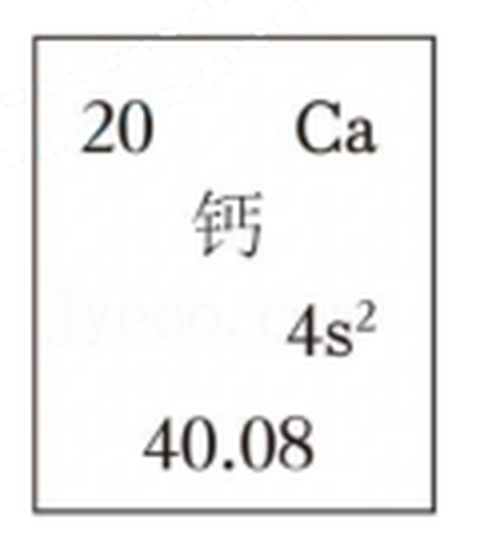
\includegraphics[width=1.7cm]{figures/ca_element_box.png}
\end{center}

\choicepairs
  {如图中 40.08 指钙元素的相对原子质量}
  {${}^{41}\mathrm{Ca}$ 的半衰期长，说明 ${}^{41}\mathrm{Ca}$ 难以失去电子}
  {${}^{41}\mathrm{Ca}$ 的衰变速度小于 ${}^{14}\mathrm{C}$ 的衰变速度}
  {从 Ca 原子束流中直接俘获 ${}^{41}\mathrm{Ca}$ 原子的过程属于化学变化}
\end{enumerate}

%==========================================================
\bigsection{二、胶体化学（本题共 16 分）}

\noindent\textbf{2.（16 分）}胶体在生命科学、材料科学及环境科学中具有广泛应用。近年来，各向异性胶体组装、生物大分子稳定性等研究为胶体化学开辟了新方向。

\begin{enumerate}[label=（\arabic*）]
\item 下列有关胶体的叙述中，正确的是\blank[3em]。
\choicelines
  {胶体区别于溶液的本质特征是胶体能够产生丁达尔现象}
  {将饱和 \ch{FeCl3} 溶液直接加热煮沸可制得 \ch{Fe(OH)3} 胶体}
  {不断搅拌后，\ch{Fe(OH)3} 胶体仍然能够稳定存在}
  {明矾[$\mathrm{KAl(SO_4)_2\cdot 12H_2O}$]可用于净水是利用了胶体粒子具有较好的吸附性}

\item 复核实验小组设计不同的实验对其制得的 \ch{Fe(OH)3} 胶体进行性质探究。写出制备 \ch{Fe(OH)3} 胶体的化学方程式：\blank[9em]。

\item 提纯制得的 \ch{Fe(OH)3} 胶体的装置是如图中的\blank[2.6em]。

\begin{center}
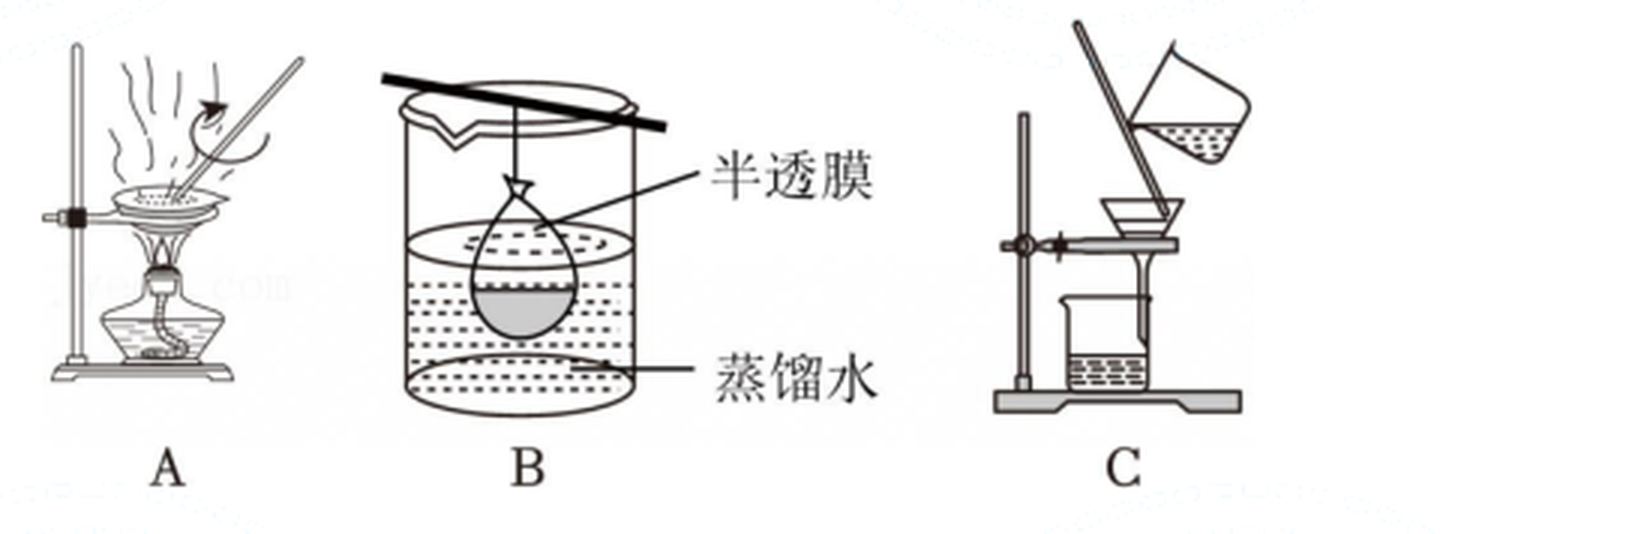
\includegraphics[width=0.80\textwidth]{figures/feoh3_purify.png}
\end{center}

\item 将提纯后的 \ch{Fe(OH)3} 胶体置于 U 形管中，通直流电一段时间后，观察到\blank[2.8em]（填“阳极”或“阴极”）附近红褐色加深，该现象称为\blank[3.4em]。

研究表明，\ch{Fe(OH)3} 胶体可净化水中低浓度的砷酸（\ch{H3AsO4}）。如图所示是不同 pH 时 \ch{Fe(OH)3} 胶体对低浓度砷酸的吸附效率曲线。

\begin{center}
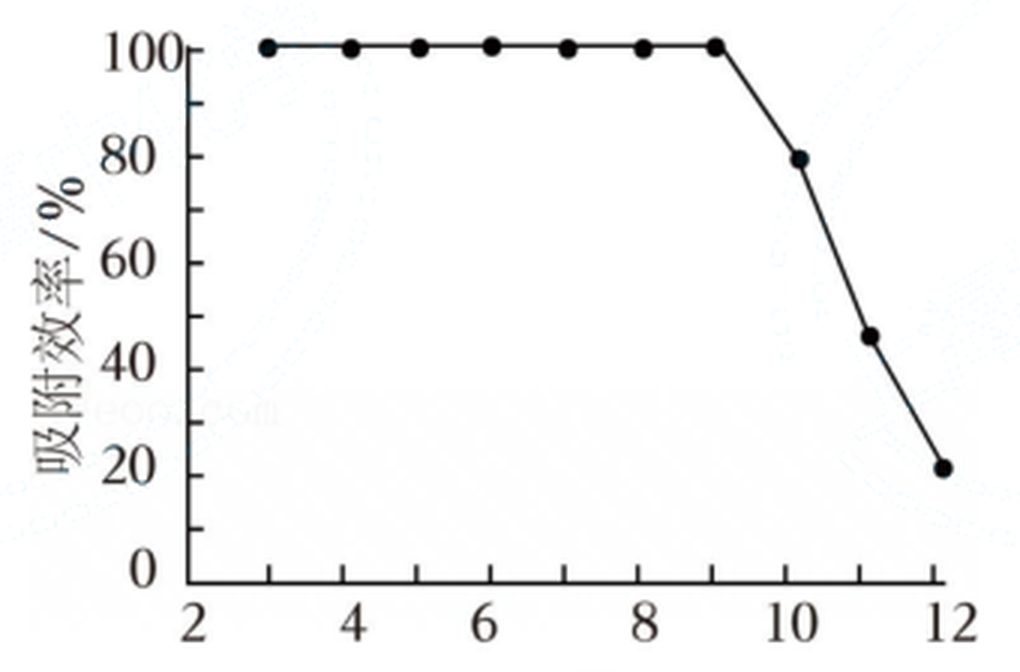
\includegraphics[width=0.42\textwidth]{figures/as_adsorption_ph.png}
\end{center}

已知：pH 反映溶液的酸碱性，pH 越高，溶液的碱性越强。pH 为 $3\sim 9$ 时，溶液中的含砷微粒主要是 $\mathrm{H_2AsO_4^-}$、$\mathrm{HAsO_4^{2-}}$。

\item pH 为 $3\sim 9$ 时，\ch{Fe(OH)3} 胶体对砷酸的吸附效率较高，其可能的原因是\blank[8em]。

\item 当水中砷酸浓度较高时，\ch{Fe(OH)3} 胶体将直接与砷酸发生化学反应生成砷酸铁（\ch{FeAsO4}）沉淀，其中砷元素是\blank[2.6em]价。$\mathrm{AsO_4^{3-}}$ 是酸根离子，则 \ch{FeAsO4} 属于\blank[3em]（填“酸”“碱”“盐”或“氧化物”）。

\item 2025 年《Nature》刊载了南方科技大学罗智团队关于氨基酸稳定胶体机制的研究。该研究发现，氨基酸（如脯氨酸、甘氨酸等）可作为稳定剂，通过吸引屏蔽机制，可逆地吸附在蛋白质、DNA 或纳米颗粒等胶体粒子的特定表面位点，削弱胶体粒子间的吸引力，从而显著提升胶体分散系的稳定性。这与电解质（如 \ch{NaCl}、\ch{Na2SO4} 等）促使胶体聚沉的作用机制相反。电解质（如 \ch{NaCl}、\ch{Na2SO4} 等）促使胶体聚沉的作用机制是\blank[8em]。

\item 蛋白药物制剂属于胶体分散系，其常常因蛋白质的相互聚集而失去药效。为了延长药物的有效期，免疫球蛋白制剂（如 Cuvitru\textsuperscript{\textregistered}）中常添加脯氨酸和甘氨酸。根据上述研究，阐述其延长有效期的主要原理是\blank[8em]。
\end{enumerate}

%==========================================================
\bigsection{三、海洋资源（本题共 25 分）}

\noindent\textbf{3.（25 分）}海洋是一座资源的宝库，化学工业中的许多基础原料都来自海洋。

\begin{enumerate}[label=（\arabic*）]
\item 海水淡化可缓解淡水资源匮乏问题。如图为太阳能海水淡化装置，该装置利用的原理是\blank[3.8em]（填分离操作名称）。

\begin{center}
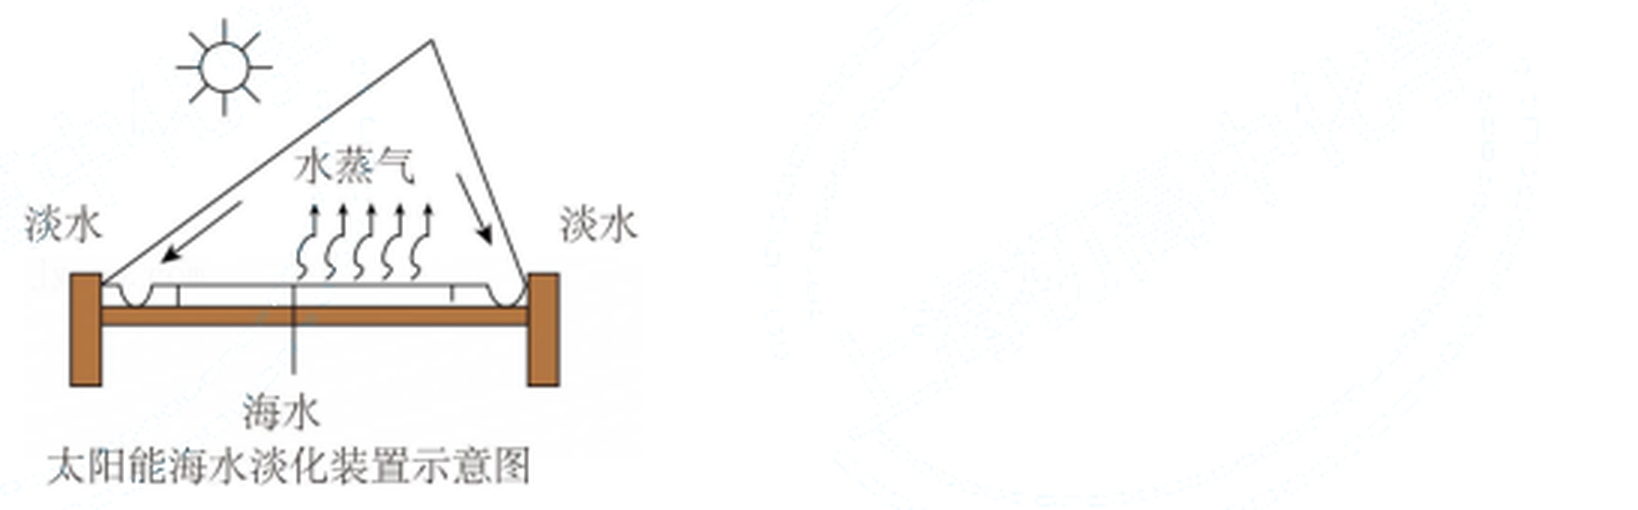
\includegraphics[width=0.52\textwidth]{figures/solar_desalination.png}
\end{center}

\item 利用海洋资源海带可以提取碘。实验室采用“萃取分液”的方法分离碘单质与有机溶剂。以下相关操作错误的是\blank[2.6em]。
% 注：该四联图中的第四个标签原卷即误印为「B.分液」（应为 D.分液），此处照原卷保留，未作改动。

\begin{center}
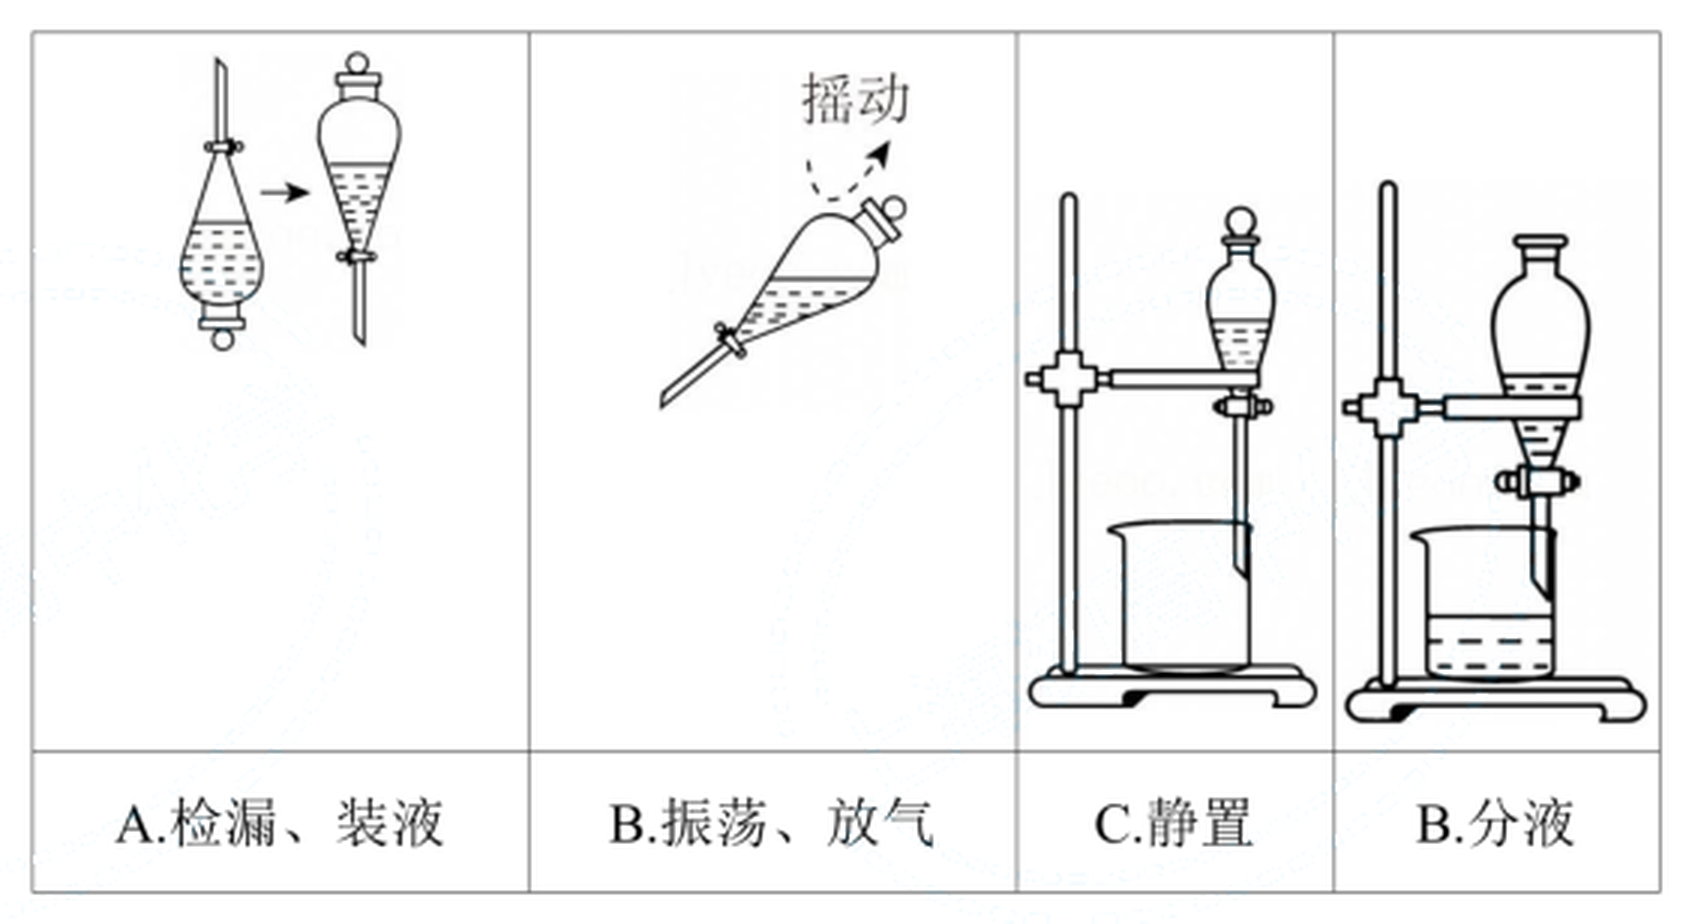
\includegraphics[width=0.68\textwidth]{figures/iodine_extraction.png}
\end{center}

\item 萃取碘水中的碘单质，可以选择的萃取剂种类很多，但不包括\blank[3em]（不定项）。
\choice{酒精}{四氯化碳}{苯}{\ch{NaCl} 溶液}

$\mathrm{SO_4^{2-}}$ 是海洋中硫元素的主要存在形式之一，其存在会干扰海水中 $\mathrm{Cl^-}$ 的检验。

\item 检验海水中 $\mathrm{Cl^-}$ 的方法是\blank[10em]。

\item 某 \ch{Na2SO4} 溶液中含有少量 \ch{Na2CO3}，已知 \ch{Na2SO4} 和 \ch{Na2CO3} 的溶解度曲线如图所示，则从该溶液中获得 $\mathrm{Na_2SO_4\cdot 10H_2O}$ 的操作是加入\blank[5em]后，\blank[4em]、\blank[4em]、过滤、洗涤、干燥。

\begin{center}
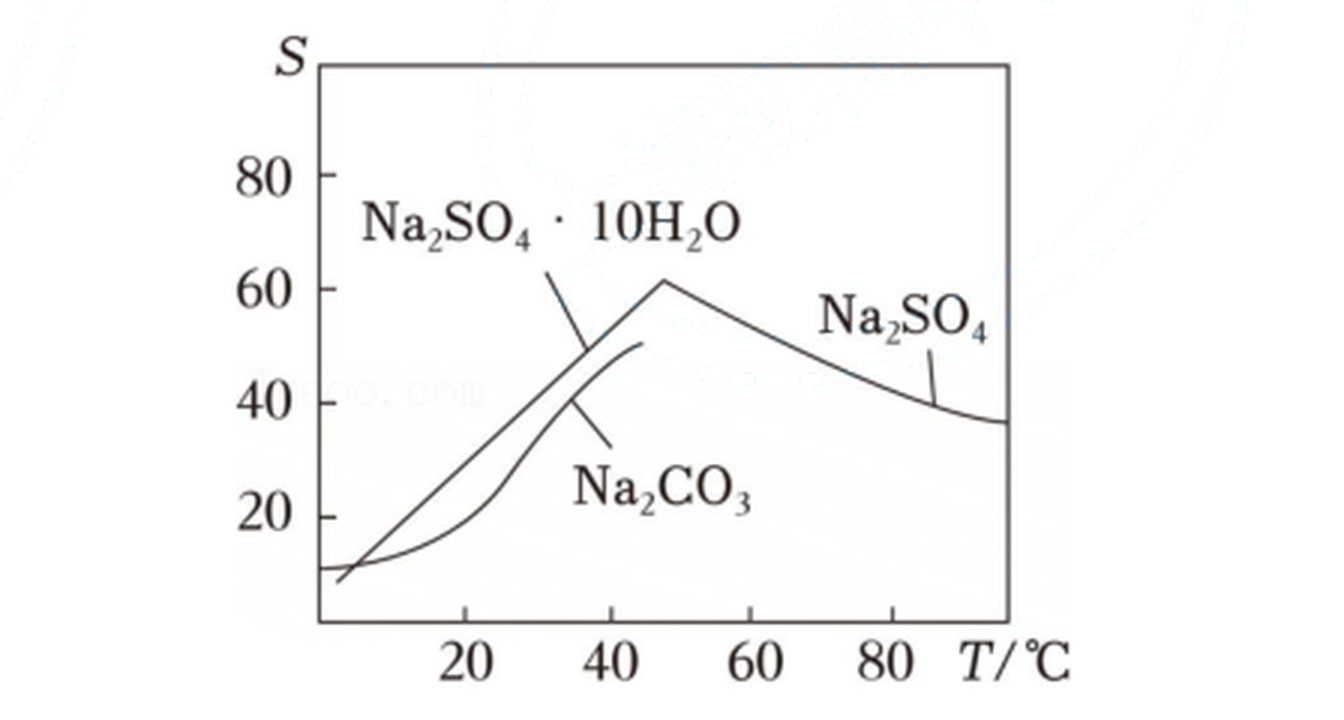
\includegraphics[width=0.48\textwidth]{figures/solubility_na2so4.png}
\end{center}

\item 以海水为原料可制取“84”消毒液。如图所示为某市售“84”消毒液标签上的部分数据，请回答下列问题。

\begin{center}
\begin{tabular}{|l|}
\hline
\rule{0pt}{1.3em}【有效成分】\ch{NaClO} \\
\hline
\rule{0pt}{1.3em}【质量分数】24\% \\
\hline
\rule{0pt}{1.3em}【溶液密度】1.18 g/cm\textsuperscript{3} \\
\hline
\rule{0pt}{1.3em}【净含量】1000 mL \\
\hline
\end{tabular}
\end{center}

该“84”消毒液的物质的量浓度约为\blank[3.4em] mol$\cdot$L\textsuperscript{$-$1}（结果保留 1 位小数）。

\item \textcircled{1} 欲配制 80 mL 2.000 mol$\cdot$L\textsuperscript{$-$1} \ch{NaClO} 溶液，需准确称量 \ch{NaClO} 固体\blank[3.4em] g。

\textcircled{2} 配制该溶液过程中所用玻璃仪器有烧杯、玻璃棒、\blank[6em]（填仪器名称）。

\item 如图是配制溶液的几个关键实验步骤和操作。

\begin{center}
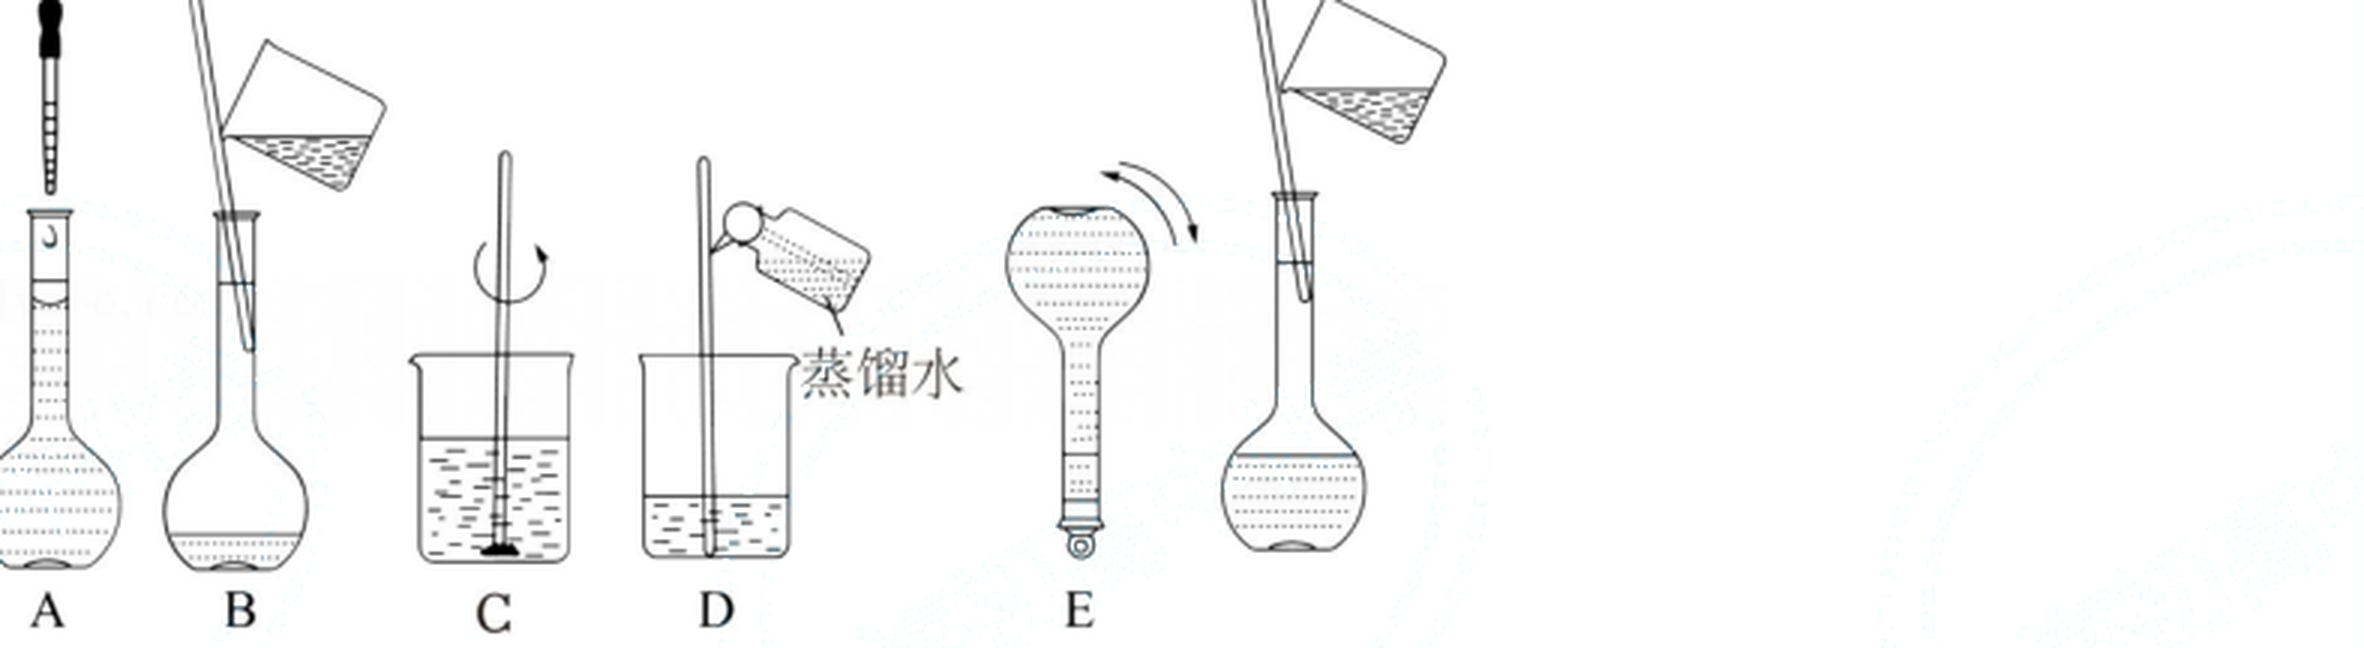
\includegraphics[width=0.88\textwidth]{figures/dilution_steps.png}
\end{center}

将上述实验步骤 A$\sim$E 按实验过程先后次序排列\blank[6em]。

\item 若所配制的次氯酸钠溶液浓度偏低，原因可能是\blank[3em]（不定项）。
\choicelines
  {配制前，容量瓶中有少量蒸馏水}
  {洗涤液未转移到容量瓶中}
  {定容时，仰视刻度线}
  {定容摇匀后，有少量溶液外流}

\item “84”消毒液与稀硫酸混合使用可增强消毒能力，某消毒小组人员用 98\%（密度为 1.84 g$\cdot$cm\textsuperscript{$-$3}）的浓硫酸配制 250 mL 2.3 mol$\cdot$L\textsuperscript{$-$1} 的稀硫酸用于增强“84”消毒液的消毒能力。需要浓硫酸的体积为\blank[3.4em] mL（保留 1 位小数）。

\item 若在用浓硫酸配制稀硫酸时，将量筒、烧杯、玻璃棒均洗涤 $2\sim 3$ 次，并将洗涤液转入容量瓶，会造成所配制的稀硫酸的浓度\blank[2.6em]。
\choicethree{偏高}{偏低}{无影响}
\end{enumerate}

%==========================================================
\bigsection{四、\ch{CuSO4} 溶液（本题共 19 分）}

\noindent\textbf{4.（19 分）}旦旦实验小组为测定 \ch{CuSO4} 溶液的浓度，设计了两个方案。

\noindentⅠ. 甲方案：取 25 mL \ch{CuSO4} 溶液，加入足量 \ch{BaCl2} 溶液，待沉淀完全后，经过滤、洗涤、干燥，得到干燥纯净的 \ch{BaSO4}，称量。

\begin{enumerate}[label=（\arabic*）]
\item 若固体质量为 $w$ g，则 $c(\mathrm{CuSO_4})=$\blank[7em] mol$\cdot$L\textsuperscript{$-$1}（不用化简）。

\item[] \noindentⅡ. 乙方案。实验步骤：

\begin{center}
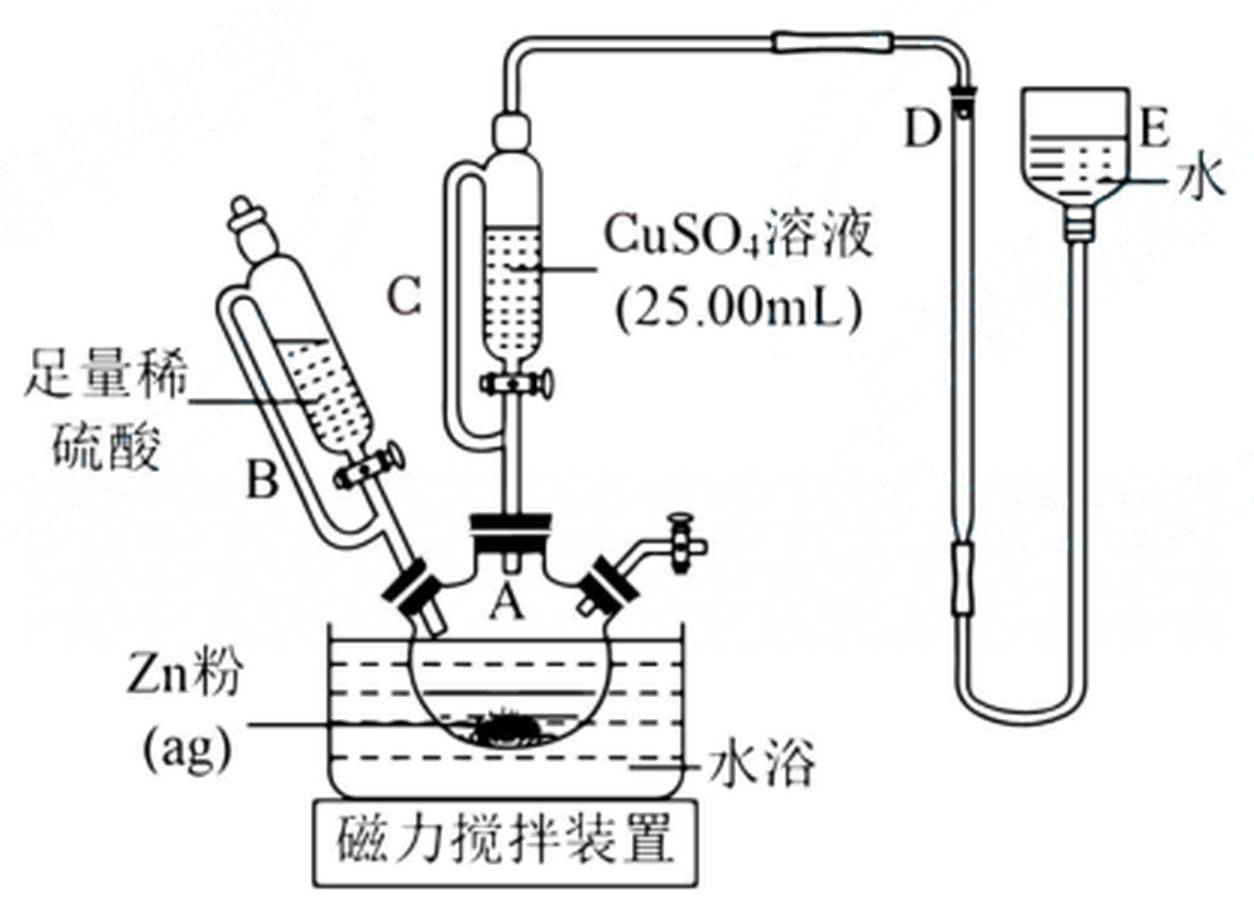
\includegraphics[width=0.46\textwidth]{figures/h2_volume_apparatus.png}
\end{center}

\begin{enumerate}[label=\textcircled{\arabic*},leftmargin=2.6em,itemsep=0.2em,topsep=0.2em]
\item 按如图安装装置（加持仪器略去）
\item ……
\item 在仪器 A、B、C、D、E 中加入如图所示的试剂
\item 调整 D、E 中两液面相平，使 D 中液面保持在 0 或略低于 0 的刻度位置，读数并记录
\item 将 \ch{CuSO4} 溶液滴入 A 中并搅拌，反应完成后，再滴加稀硫酸至体系中不再有气体产生
\item 待体系恢复到室温，移动 E 管，保持 D、E 中两液面相平，读数并记录
\item 处理数据
\end{enumerate}

\item 步骤\textcircled{2} 为\blank[8em]。

\item Zn 粉质量为 $a=0.195$ g，若测得 \ch{H2} 体积为 22.40 mL（已折算为标准状况下的体积），则\blank[8em]（写出必要的计算步骤）
\workspace[5]

\item 若步骤\textcircled{6} E 管液面高于 D 管，未调节液面即读数，则测得 $c(\mathrm{CuSO_4})=$\blank[3em]。
\choice{偏大}{偏小}{无影响}{无法判断}

\item 是否能用同样的装置和方法测定 \ch{MgSO4} 的浓度：\blank[2.6em]（填“是”或“否”）原因是\blank[6em]。

\item 如果 \ch{CuSO4} 浓度的参考值为 0.100 mol/L，而测定结果是 0.096 mol/L，则测定的相对偏差为\blank[3em]。

\item \ch{CuSO4} 溶液经过一系列操作，可以获得 $\mathrm{CuSO_4\cdot 5H_2O}$。取 2.50 g $\mathrm{CuSO_4\cdot 5H_2O}$ 受热脱水过程的热重曲线（样品质量随温度变化的曲线）如图所示。

\begin{center}
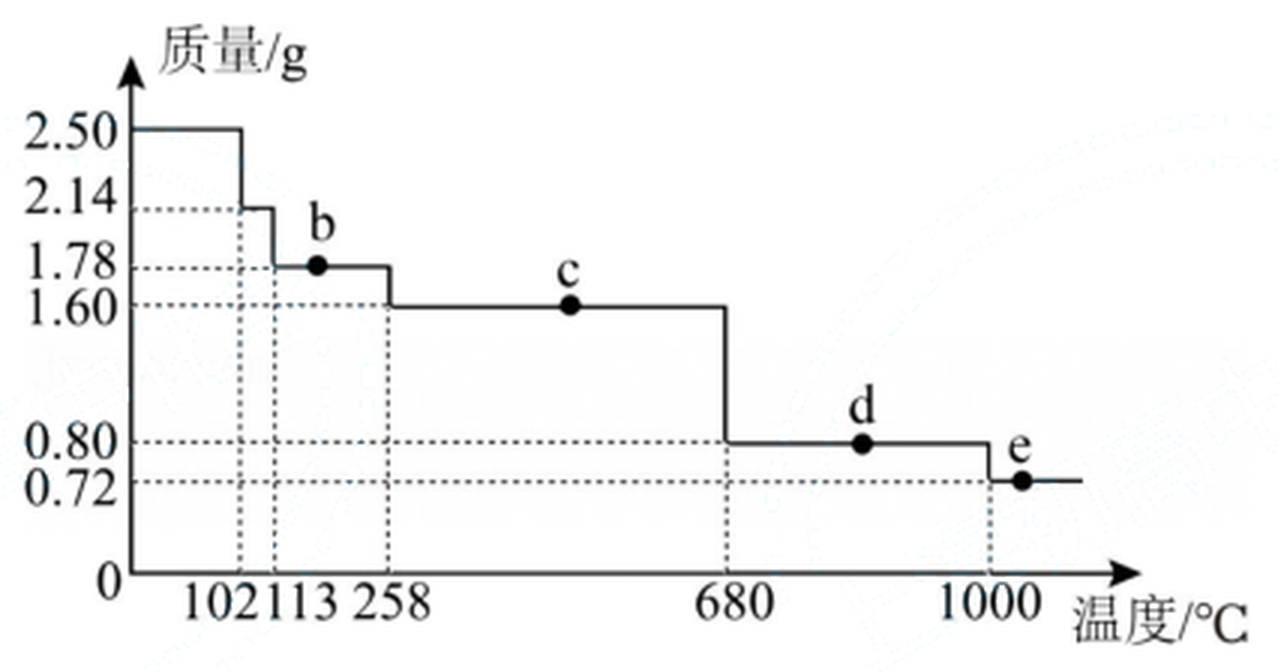
\includegraphics[width=0.48\textwidth]{figures/tga_cuso4.png}
\end{center}

请回答下列问题：b 点时固体物质的化学式\blank[5em]。

\item 取 270 ℃ 所得样品，于 770 ℃ 灼烧得到的主要产物是黑色粉末和 \ch{SO3}，该反应的化学方程式为\blank[9em]。

\item 1000 ℃ 发生反应的化学方程式为\blank[9em]。
\end{enumerate}

%==========================================================
\bigsection{五、物质的量（本题共 16 分）}

\noindent\textbf{5.（16 分）}物质的量是将微观粒子数与宏观可称量物理量联系起来的桥梁，极大地促进了化学学科的发展。

\begin{enumerate}[label=（\arabic*）]
\item 某次高空探测，收集到含 \ch{O3}、\ch{O2}、\ch{N2}（其他气体忽略不计）的大气样本，在实验室中微热一段时间后，\ch{O3} 全部转化为 \ch{O2}（$2\mathrm{O_3}=3\mathrm{O_2}$）。若气体总体积增加了 0.36\%，则大气样本中 \ch{O3} 的体积分数为\blank[3.4em]（反应前后温度和压强均保持不变）。

\item 物质 R 吸收氢气后成为 $\mathrm{RH_6}$，$\mathrm{RH_6}$ 晶体中的氢密度可达到 $1.1\times 10^{3}$ g$\cdot$m\textsuperscript{$-$3}（氢密度是指单位体积晶体中氢元素的质量），则此时 1 m\textsuperscript{3} 晶体中所储的氢相当于标准状况下\blank[5em] L 氢气。

\item 如图所示，一密闭容器被无摩擦、可自由滑动的两隔板 a、b 分成甲、乙两室；标准状况下，在乙室中充入 \ch{NH3} 0.4 mol，甲室中充入 \ch{HCl}、\ch{N2} 的混合气体，静止时隔板位置如图所示。已知甲、乙两室中气体的质量差为 17.3 g。

\begin{center}
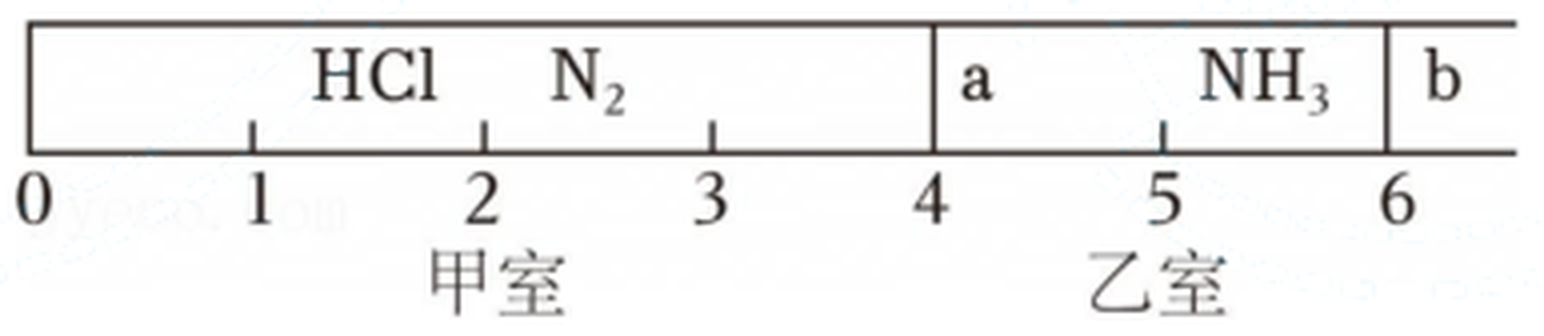
\includegraphics[width=0.62\textwidth]{figures/two_chamber_tube.png}
\end{center}

\textcircled{1} 甲室中气体总质量为\blank[3.4em] g。

\textcircled{2} 甲室中 \ch{HCl}、\ch{N2} 的物质的量之比为\blank[3em]。

\textcircled{3} 将隔板 a 去掉，当 \ch{HCl} 与 \ch{NH3} 充分反应生成 \ch{NH4Cl} 固体后（仅发生此反应），隔板 b 将位于刻度“\blank[3em]”处（填数字，不考虑固体物质产生的体积），此时体系的平均相对分子质量为\blank[3.4em]。

\item 火箭发射后，发射场附近废水中偏二甲肼（\ch{C2H8N2}）浓度变高，可用 \ch{H2O2} 对废水处理。处理 100 L 的 2000 mg/L 偏二甲肼废水，使用密度为 1.11 g/mL 30\% 的 \ch{H2O2} 溶液，则 \ch{H2O2} 溶液的理论投加量为\blank[3.4em] L（保留两位小数）。

已知：$\mathrm{C_2H_8N_2(l)+8H_2O_2(l)=N_2(g)+2CO_2(g)+12H_2O(l)}$

\item 焦亚硫酸钠（\ch{Na2S2O5}）易溶于水，与强酸反应放出较多 \ch{SO2}。\ch{Na2S2O5} 作为食品添加剂，在葡萄酒中残留量一般不得超过 0.25 g$\cdot$L\textsuperscript{$-$1}（以 \ch{SO2} 计）。小复同学检测葡萄酒样品中 \ch{Na2S2O5} 残留量，实验如下：取 150 mL 葡萄酒样品，加稀硫酸酸化后加热，将产生气体通入足量双氧水中充分吸收，再除去过量的 \ch{H2O2}，冷却后，用 0.100 mol$\cdot$L\textsuperscript{$-$1} \ch{NaOH} 溶液与上述吸收液反应，恰好反应时消耗 \ch{NaOH} 溶液 15.00 mL，则该样品中 \ch{Na2S2O5} 的残留量为\blank[4em] g$\cdot$L\textsuperscript{$-$1}（残留量以 \ch{SO2} 计）。

已知：$\mathrm{SO_2+H_2O_2=H_2SO_4}$
\workspace[6]
\end{enumerate}

%==========================================================
% 以下「参考答案」整节仅在答案版输出（试卷版由 \ifanswer 整段吞掉）
\ifanswer
\newpage
\bigsection{参考答案}

\begin{enumerate}[label=\textbf{\arabic*.},leftmargin=2.5em]
\item
\begin{enumerate}[label=（\arabic*）]
\item D；
\item $A-x+n+24$；
\item B；
\item C；
\item AD（不定项）；
\item 氚。A 为氢元素，其核素中质子数（1）为中子数（2）的一半，即 ${}_{1}^{3}\mathrm{H}$；
\item $\left[\mathrm{H}:\right]^-$（$\mathrm{H^-}$ 的电子式）；$\mathrm{Mg^{2+}}$ 的结构示意图为
\begin{center}
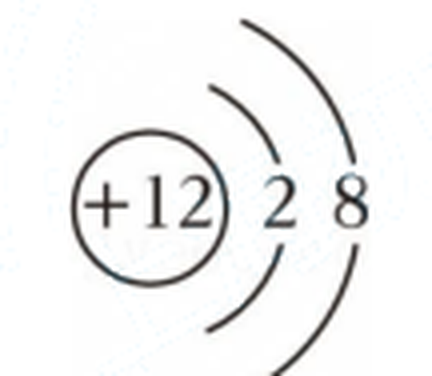
\includegraphics[width=1.1cm]{figures/mg2_plus_shell.png}
\end{center}
\item $\mathrm{SO_2+2NaOH=Na_2SO_3+H_2O}$（$EB_2$ 为 \ch{SO2}，$CBA$ 为 \ch{NaOH}）；
\item $a=7.58$，$b=49.82$；
\item AC（不定项）。
\end{enumerate}

\item
\begin{enumerate}[label=（\arabic*）]
\item D；
\item $\mathrm{FeCl_3+3H_2O}\xrightarrow{\Delta}\mathrm{Fe(OH)_3(\text{胶体})+3HCl}$；% \Delta 不可写在 \mathrm{} 内，否则映射到 Times New Roman 缺字形
\item B；
\item 阴极；电泳；
\item pH 为 $3\sim 9$ 时，溶液中的含砷微粒主要是 $\mathrm{H_2AsO_4^-}$、$\mathrm{HAsO_4^{2-}}$，\ch{Fe(OH)3} 胶体粒子带正电荷，能吸附带负电荷的 $\mathrm{H_2AsO_4^-}$、$\mathrm{HAsO_4^{2-}}$；
\item $+5$ 价；盐；
\item 向胶体中加入盐时，其中的阳离子或阴离子能中和分散质微粒所带的电荷，从而使分散质聚集成较大的微粒，在重力作用下形成沉淀析出；
\item 氨基酸通过阻碍颗粒间直接接触，增强胶体颗粒间的排斥作用来抑制胶体聚集。
\end{enumerate}

\item
\begin{enumerate}[label=（\arabic*）]
\item 蒸馏（填分离操作名称）；
\item B；
\item AD（不定项）；
\item 取少量海水于试管中，向其中加入 \ch{Ba(NO3)2} 溶液，静置，向上层清液中（或取上层清液）加入 \ch{HNO3} 酸化的 \ch{AgNO3} 溶液，若有白色沉淀生成，说明海水中有 $\mathrm{Cl^-}$；
\item 硫酸至不再产生气泡；蒸发浓缩、冷却结晶；
\item 3.8 mol$\cdot$L\textsuperscript{$-$1}（结果保留 1 位小数）；
\item \textcircled{1} 14.9 g；\textcircled{2} 胶头滴管、100 mL 容量瓶（填仪器名称）；
\item CBDBAE；
\item BC（不定项）；
\item 31.3 mL（保留 1 位小数）；
\item A。
\end{enumerate}

\item
\begin{enumerate}[label=（\arabic*）]
\item $\dfrac{40w}{233}$ mol$\cdot$L\textsuperscript{$-$1}（不用化简）；
\item 检查装置的气密性；
\item $0.08$ mol/L（写出必要的计算步骤）；
\item A；
\item 否（填“是”或“否”）；原因是 Mg 比 Zn 活泼，Zn 与 \ch{MgSO4} 不反应；
\item 4\%；
\item $\mathrm{CuSO_4\cdot H_2O}$；
\item $\mathrm{CuSO_4\xrightarrow{770\,^{\circ}\mathrm{C}}CuO+SO_3\uparrow}$；
\item $\mathrm{4CuO\xrightarrow{1000\,^{\circ}\mathrm{C}}2Cu_2O+O_2\uparrow}$。
\end{enumerate}

\item
\begin{enumerate}[label=（\arabic*）]
\item 0.72\%（反应前后温度和压强均保持不变）；
\item $1.232\times 10^{6}$ L 氢气；
\item \textcircled{1} 24.1 g；\textcircled{2} $1:3$；\textcircled{3} 4；25.25；
\item 2.72 L（保留两位小数）；
\item 0.320 g$\cdot$L\textsuperscript{$-$1}（残留量以 \ch{SO2} 计）。
\end{enumerate}
\end{enumerate}
\fi

\end{document}
"

\documentclass[11pt,a4paper]{article}
\usepackage{chem}

% ---- 卷名（页眉；答案版自动追加版本标记）----
\newcommand{\paperhead}{2025-2026 学年上海市复旦附中高一（上）月考化学试卷（10 月份）}
\fancyhead[L]{\small\kaishu \paperhead\vermark}

% ---- 标题 ----
\title{\heiti\bfseries\Large \paperhead}
\author{}
\date{}

% 原卷部分题干下方留有整段演算空白，此处预留书写空间（仅试卷版输出）
\newcommand{\workspace}[1][6]{\ansspace[#1]}

\begin{document}
\maketitle
\thispagestyle{fancy}

%==========================================================
\bigsection{一、原子结构（本题共 24 分）}

\noindent\textbf{1.（24 分）}人类对原子结构的认识是一段充满智慧的探索历程。

\begin{enumerate}[label=（\arabic*）]
\item 原子的构成及核外电子排布情况可用原子结构示意图表示，其依据是下面哪位科学家的原子结构模型\blank[2.6em]。
\choice{道尔顿}{汤姆孙}{卢瑟福}{玻尔}

\item 在 $RO_3^{n-}$ 中，共有 $x$ 个核外电子，R 原子的质量数为 $A$，则 R 原子核内含有的中子数是\blank[4em]。
\workspace[3]

\item 下列各组微粒中，具有相同质子数和电子数的一组微粒是\blank[3em]。
\choicepairs
  {$\mathrm{OH^-}$、$\mathrm{F^-}$、$\mathrm{Ne}$、$\mathrm{O^{2-}}$}
  {\ch{H2O}、\ch{CH4}、\ch{NH3}、\ch{Ne}}
  {$\mathrm{H_3O^+}$、$\mathrm{Na^+}$、$\mathrm{NH_4^+}$、$\mathrm{Mg^{2+}}$}
  {$\mathrm{O^{2-}}$、$\mathrm{F^-}$、$\mathrm{Mg^{2+}}$、$\mathrm{Al^{3+}}$}

\item 下列说法正确的是\blank[3em]。
\choicelines
  {电子在原子核外空间高速运动且能量都相等}
  {两种微粒的核外电子排布相同，则一定属于同种元素}
  {K 层上运动的电子的能量最低}
  {某原子 M 层电子数为 L 层电子数的 4 倍}

\item 锂在核工业中应用广泛，如 ${}_{3}^{6}\mathrm{Li}$ 和 ${}_{3}^{7}\mathrm{Li}$ 可作核反应堆最佳热载体，${}_{3}^{7}\mathrm{LiH}$ 和 ${}_{3}^{7}\mathrm{LiD}$ 用作高温堆减速剂。下列有关说法错误的是\blank[3em]（不定项）。
\choicepairs
  {${}_{3}^{6}\mathrm{Li}$ 和 ${}_{3}^{7}\mathrm{Li}$ 是同种核素}
  {${}_{3}^{7}\mathrm{LiH}$ 和 ${}_{3}^{7}\mathrm{LiD}$ 化学性质几乎完全相同}
  {${}_{3}^{7}\mathrm{LiH}$ 和 ${}_{3}^{7}\mathrm{LiD}$ 中质子总数相同}
  {${}_{3}^{6}\mathrm{Li}$ 和 ${}_{3}^{7}\mathrm{Li}$ 是同素异形体}
\end{enumerate}

有 A、B、C、D、E 五种元素，它们的核电荷数依次增大，且都小于 18。其中只有 C、D 为金属元素；A 和 C 的最外层均只有 1 个电子；B 和 E 的最外层电子数相同，且 B 的 L 层电子数是 K 层电子数的 3 倍；D 的最外层电子数为 E 的最外层电子数的 $\dfrac{1}{3}$。完成下列问题：

\begin{enumerate}[label=（\arabic*）,start=6]
\item A 的一种核素中质子数为中子数的一半，则该核素的名称是\blank[4em]。% 原卷作「则该核素的名称分别为______。」，其中「分别」与答案（仅一个核素「氚」）矛盾，此处删去「分别」二字，其余照原卷

\item A 形成的简单负离子的电子式为\blank[4em]；D 形成的简单正离子的结构示意图为\blank[4em]。

\item 写出少量 $EB_2$ 与 $CBA$ 溶液反应的化学方程式：\blank[8em]。

\item 硒元素的天然同位素组成如表：

\begin{center}
\begin{tabular}{|c|c|c|c|c|c|c|}
\hline
\rule{0pt}{1.3em}核素的质量数 & 74 & 76 & 77 & 78 & 80 & 82 \\
\hline
\rule{0pt}{1.3em}核素的丰度（\%） & 0.87 & 9.02 & $a$ & 23.52 & $b$ & 9.19 \\
\hline
\end{tabular}
\end{center}

已知硒元素的近似相对原子质量为 79.073，则 $a=$\blank[3.2em]，$b=$\blank[3.2em]。

\item 我国科研人员利用激光操控方法，从 Ca 原子束流中直接俘获 ${}^{41}\mathrm{Ca}$ 原子，实现了对同位素 ${}^{41}\mathrm{Ca}$ 的灵敏检测。${}^{41}\mathrm{Ca}$ 的半衰期（放射性元素的原子核有半数发生衰变所需的时间）长达 10 万年，是 ${}^{14}\mathrm{C}$ 的 17 倍，可应用于地球科学与考古学。下列说法正确的是\blank[3em]（不定项）。

\begin{center}
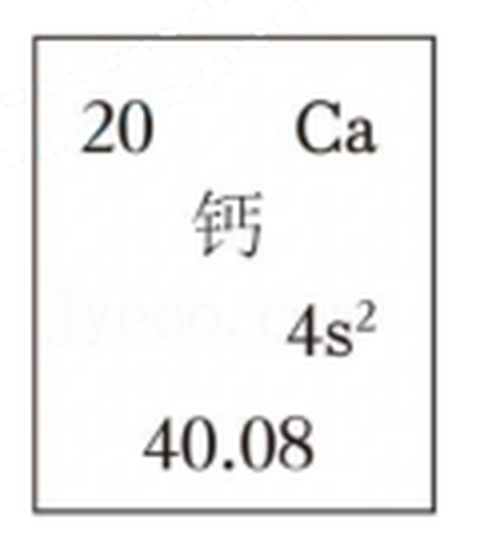
\includegraphics[width=1.7cm]{figures/ca_element_box.png}
\end{center}

\choicepairs
  {如图中 40.08 指钙元素的相对原子质量}
  {${}^{41}\mathrm{Ca}$ 的半衰期长，说明 ${}^{41}\mathrm{Ca}$ 难以失去电子}
  {${}^{41}\mathrm{Ca}$ 的衰变速度小于 ${}^{14}\mathrm{C}$ 的衰变速度}
  {从 Ca 原子束流中直接俘获 ${}^{41}\mathrm{Ca}$ 原子的过程属于化学变化}
\end{enumerate}

%==========================================================
\bigsection{二、胶体化学（本题共 16 分）}

\noindent\textbf{2.（16 分）}胶体在生命科学、材料科学及环境科学中具有广泛应用。近年来，各向异性胶体组装、生物大分子稳定性等研究为胶体化学开辟了新方向。

\begin{enumerate}[label=（\arabic*）]
\item 下列有关胶体的叙述中，正确的是\blank[3em]。
\choicelines
  {胶体区别于溶液的本质特征是胶体能够产生丁达尔现象}
  {将饱和 \ch{FeCl3} 溶液直接加热煮沸可制得 \ch{Fe(OH)3} 胶体}
  {不断搅拌后，\ch{Fe(OH)3} 胶体仍然能够稳定存在}
  {明矾[$\mathrm{KAl(SO_4)_2\cdot 12H_2O}$]可用于净水是利用了胶体粒子具有较好的吸附性}

\item 复核实验小组设计不同的实验对其制得的 \ch{Fe(OH)3} 胶体进行性质探究。写出制备 \ch{Fe(OH)3} 胶体的化学方程式：\blank[9em]。

\item 提纯制得的 \ch{Fe(OH)3} 胶体的装置是如图中的\blank[2.6em]。

\begin{center}
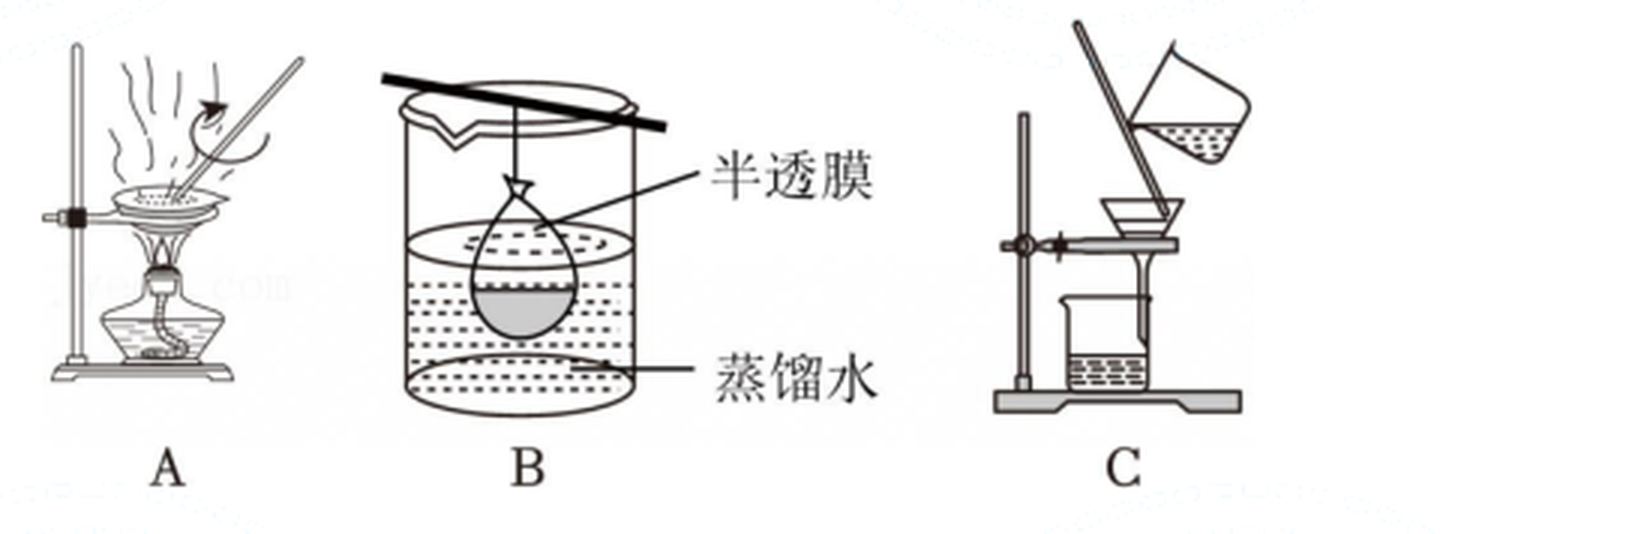
\includegraphics[width=0.80\textwidth]{figures/feoh3_purify.png}
\end{center}

\item 将提纯后的 \ch{Fe(OH)3} 胶体置于 U 形管中，通直流电一段时间后，观察到\blank[2.8em]（填“阳极”或“阴极”）附近红褐色加深，该现象称为\blank[3.4em]。

研究表明，\ch{Fe(OH)3} 胶体可净化水中低浓度的砷酸（\ch{H3AsO4}）。如图所示是不同 pH 时 \ch{Fe(OH)3} 胶体对低浓度砷酸的吸附效率曲线。

\begin{center}
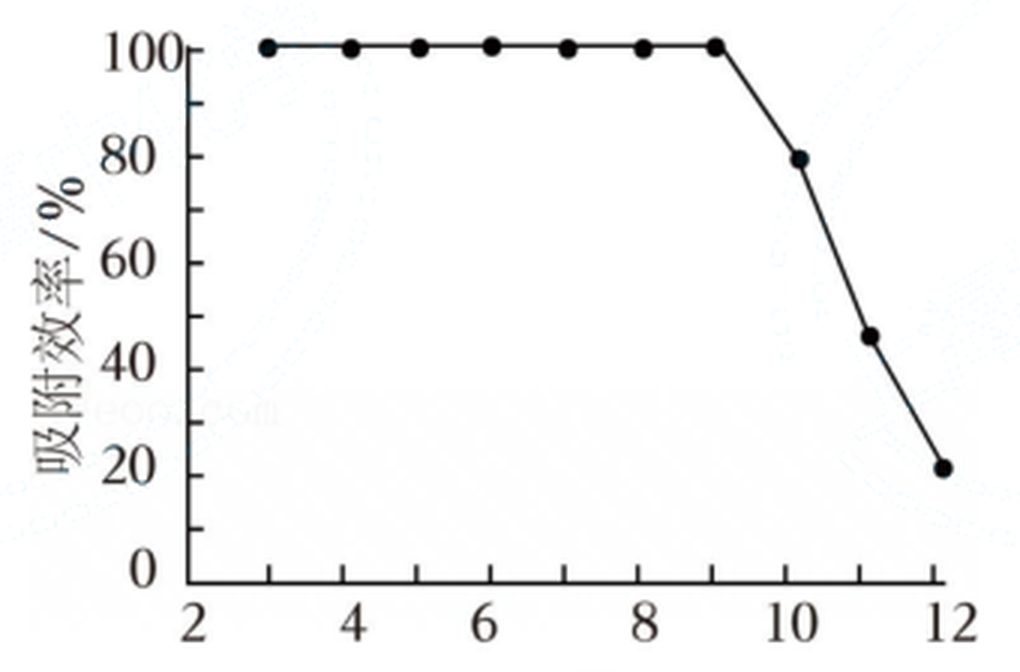
\includegraphics[width=0.42\textwidth]{figures/as_adsorption_ph.png}
\end{center}

已知：pH 反映溶液的酸碱性，pH 越高，溶液的碱性越强。pH 为 $3\sim 9$ 时，溶液中的含砷微粒主要是 $\mathrm{H_2AsO_4^-}$、$\mathrm{HAsO_4^{2-}}$。

\item pH 为 $3\sim 9$ 时，\ch{Fe(OH)3} 胶体对砷酸的吸附效率较高，其可能的原因是\blank[8em]。

\item 当水中砷酸浓度较高时，\ch{Fe(OH)3} 胶体将直接与砷酸发生化学反应生成砷酸铁（\ch{FeAsO4}）沉淀，其中砷元素是\blank[2.6em]价。$\mathrm{AsO_4^{3-}}$ 是酸根离子，则 \ch{FeAsO4} 属于\blank[3em]（填“酸”“碱”“盐”或“氧化物”）。

\item 2025 年《Nature》刊载了南方科技大学罗智团队关于氨基酸稳定胶体机制的研究。该研究发现，氨基酸（如脯氨酸、甘氨酸等）可作为稳定剂，通过吸引屏蔽机制，可逆地吸附在蛋白质、DNA 或纳米颗粒等胶体粒子的特定表面位点，削弱胶体粒子间的吸引力，从而显著提升胶体分散系的稳定性。这与电解质（如 \ch{NaCl}、\ch{Na2SO4} 等）促使胶体聚沉的作用机制相反。电解质（如 \ch{NaCl}、\ch{Na2SO4} 等）促使胶体聚沉的作用机制是\blank[8em]。

\item 蛋白药物制剂属于胶体分散系，其常常因蛋白质的相互聚集而失去药效。为了延长药物的有效期，免疫球蛋白制剂（如 Cuvitru\textsuperscript{\textregistered}）中常添加脯氨酸和甘氨酸。根据上述研究，阐述其延长有效期的主要原理是\blank[8em]。
\end{enumerate}

%==========================================================
\bigsection{三、海洋资源（本题共 25 分）}

\noindent\textbf{3.（25 分）}海洋是一座资源的宝库，化学工业中的许多基础原料都来自海洋。

\begin{enumerate}[label=（\arabic*）]
\item 海水淡化可缓解淡水资源匮乏问题。如图为太阳能海水淡化装置，该装置利用的原理是\blank[3.8em]（填分离操作名称）。

\begin{center}
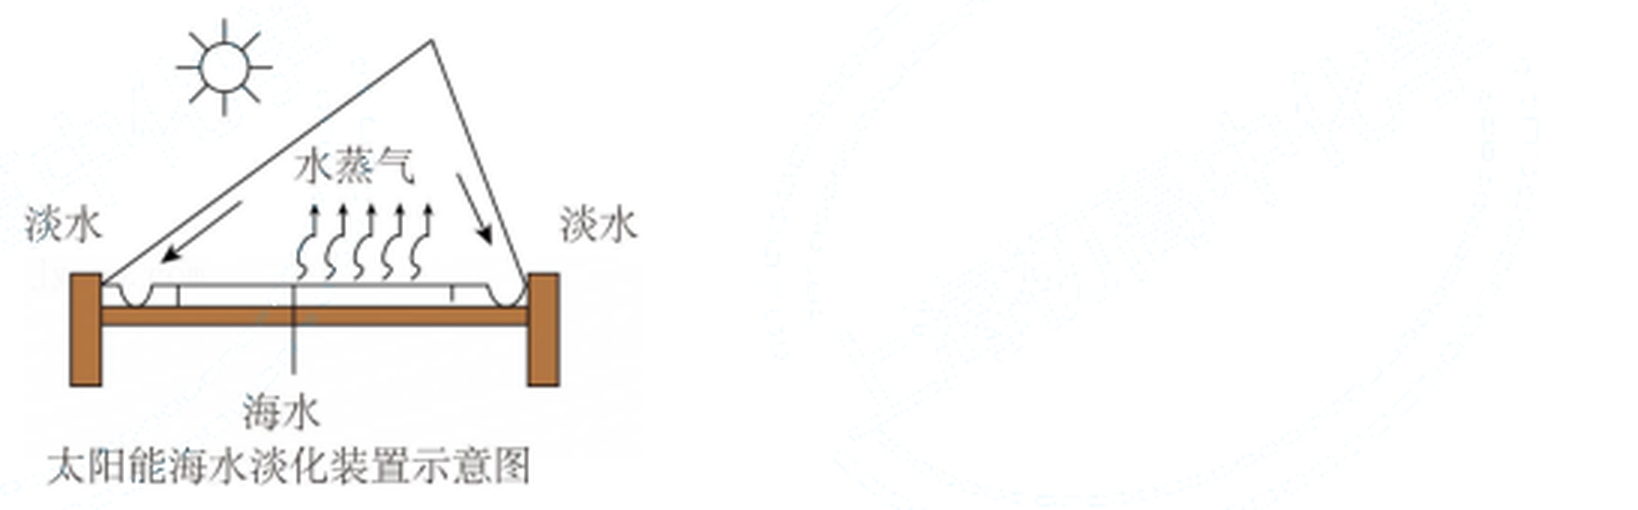
\includegraphics[width=0.52\textwidth]{figures/solar_desalination.png}
\end{center}

\item 利用海洋资源海带可以提取碘。实验室采用“萃取分液”的方法分离碘单质与有机溶剂。以下相关操作错误的是\blank[2.6em]。
% 注：该四联图中的第四个标签原卷即误印为「B.分液」（应为 D.分液），此处照原卷保留，未作改动。

\begin{center}
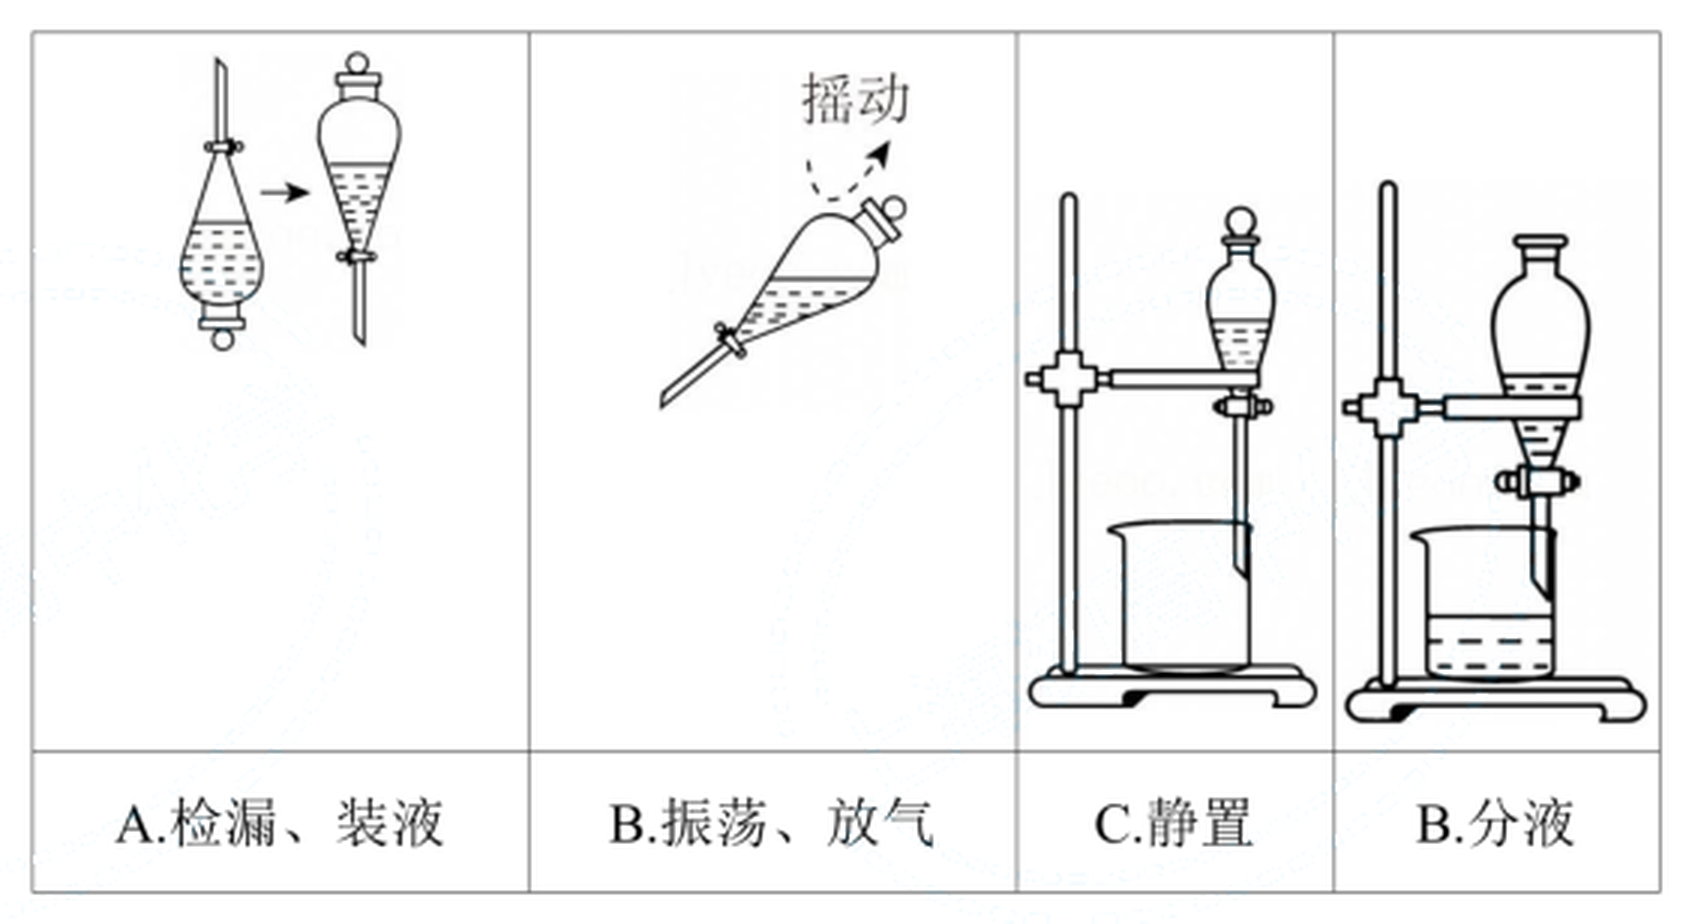
\includegraphics[width=0.68\textwidth]{figures/iodine_extraction.png}
\end{center}

\item 萃取碘水中的碘单质，可以选择的萃取剂种类很多，但不包括\blank[3em]（不定项）。
\choice{酒精}{四氯化碳}{苯}{\ch{NaCl} 溶液}

$\mathrm{SO_4^{2-}}$ 是海洋中硫元素的主要存在形式之一，其存在会干扰海水中 $\mathrm{Cl^-}$ 的检验。

\item 检验海水中 $\mathrm{Cl^-}$ 的方法是\blank[10em]。

\item 某 \ch{Na2SO4} 溶液中含有少量 \ch{Na2CO3}，已知 \ch{Na2SO4} 和 \ch{Na2CO3} 的溶解度曲线如图所示，则从该溶液中获得 $\mathrm{Na_2SO_4\cdot 10H_2O}$ 的操作是加入\blank[5em]后，\blank[4em]、\blank[4em]、过滤、洗涤、干燥。

\begin{center}
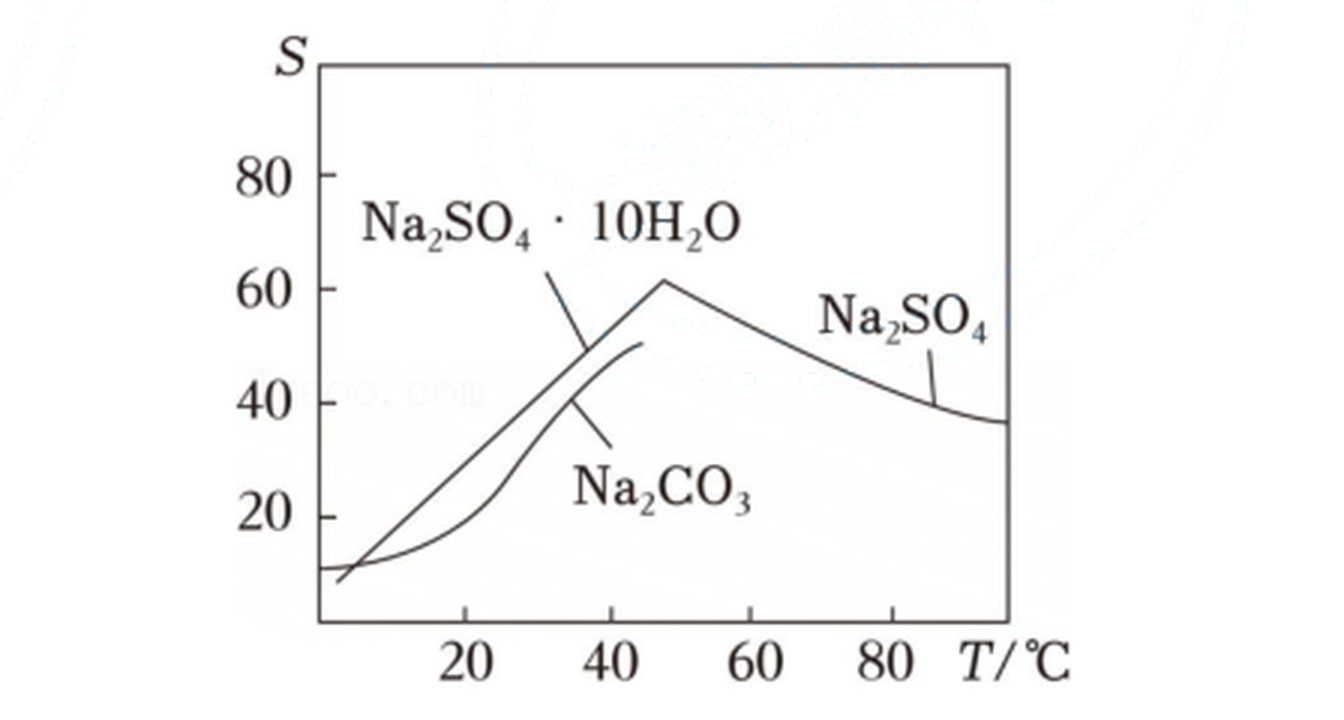
\includegraphics[width=0.48\textwidth]{figures/solubility_na2so4.png}
\end{center}

\item 以海水为原料可制取“84”消毒液。如图所示为某市售“84”消毒液标签上的部分数据，请回答下列问题。

\begin{center}
\begin{tabular}{|l|}
\hline
\rule{0pt}{1.3em}【有效成分】\ch{NaClO} \\
\hline
\rule{0pt}{1.3em}【质量分数】24\% \\
\hline
\rule{0pt}{1.3em}【溶液密度】1.18 g/cm\textsuperscript{3} \\
\hline
\rule{0pt}{1.3em}【净含量】1000 mL \\
\hline
\end{tabular}
\end{center}

该“84”消毒液的物质的量浓度约为\blank[3.4em] mol$\cdot$L\textsuperscript{$-$1}（结果保留 1 位小数）。

\item \textcircled{1} 欲配制 80 mL 2.000 mol$\cdot$L\textsuperscript{$-$1} \ch{NaClO} 溶液，需准确称量 \ch{NaClO} 固体\blank[3.4em] g。

\textcircled{2} 配制该溶液过程中所用玻璃仪器有烧杯、玻璃棒、\blank[6em]（填仪器名称）。

\item 如图是配制溶液的几个关键实验步骤和操作。

\begin{center}
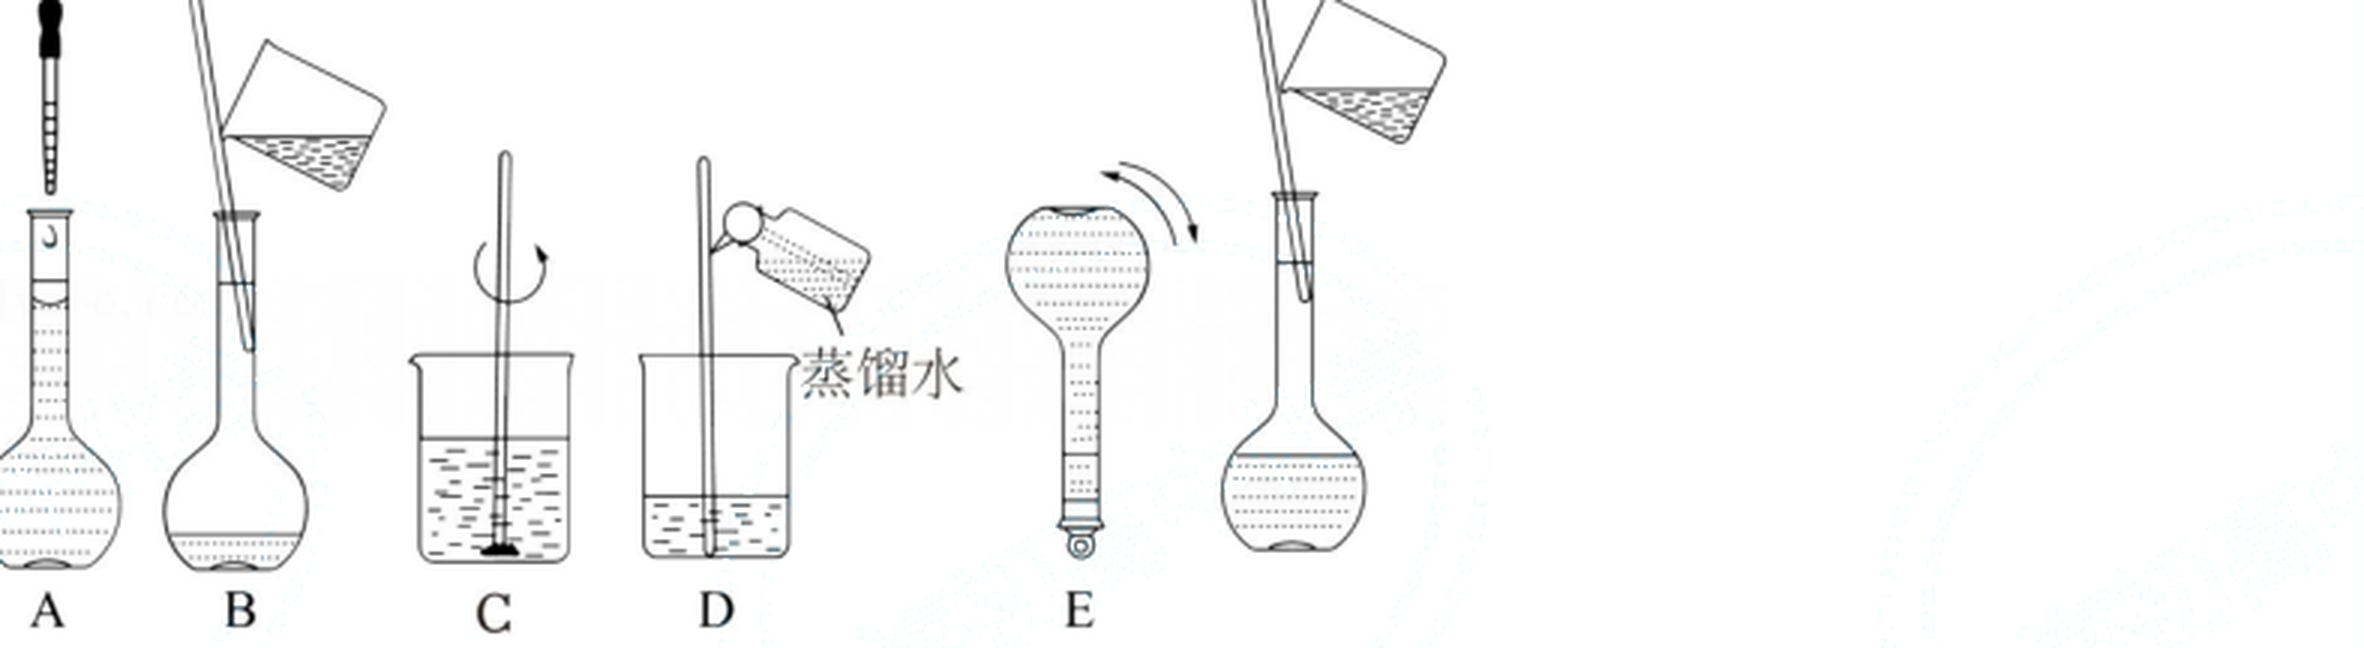
\includegraphics[width=0.88\textwidth]{figures/dilution_steps.png}
\end{center}

将上述实验步骤 A$\sim$E 按实验过程先后次序排列\blank[6em]。

\item 若所配制的次氯酸钠溶液浓度偏低，原因可能是\blank[3em]（不定项）。
\choicelines
  {配制前，容量瓶中有少量蒸馏水}
  {洗涤液未转移到容量瓶中}
  {定容时，仰视刻度线}
  {定容摇匀后，有少量溶液外流}

\item “84”消毒液与稀硫酸混合使用可增强消毒能力，某消毒小组人员用 98\%（密度为 1.84 g$\cdot$cm\textsuperscript{$-$3}）的浓硫酸配制 250 mL 2.3 mol$\cdot$L\textsuperscript{$-$1} 的稀硫酸用于增强“84”消毒液的消毒能力。需要浓硫酸的体积为\blank[3.4em] mL（保留 1 位小数）。

\item 若在用浓硫酸配制稀硫酸时，将量筒、烧杯、玻璃棒均洗涤 $2\sim 3$ 次，并将洗涤液转入容量瓶，会造成所配制的稀硫酸的浓度\blank[2.6em]。
\choicethree{偏高}{偏低}{无影响}
\end{enumerate}

%==========================================================
\bigsection{四、\ch{CuSO4} 溶液（本题共 19 分）}

\noindent\textbf{4.（19 分）}旦旦实验小组为测定 \ch{CuSO4} 溶液的浓度，设计了两个方案。

\noindentⅠ. 甲方案：取 25 mL \ch{CuSO4} 溶液，加入足量 \ch{BaCl2} 溶液，待沉淀完全后，经过滤、洗涤、干燥，得到干燥纯净的 \ch{BaSO4}，称量。

\begin{enumerate}[label=（\arabic*）]
\item 若固体质量为 $w$ g，则 $c(\mathrm{CuSO_4})=$\blank[7em] mol$\cdot$L\textsuperscript{$-$1}（不用化简）。

\item[] \noindentⅡ. 乙方案。实验步骤：

\begin{center}
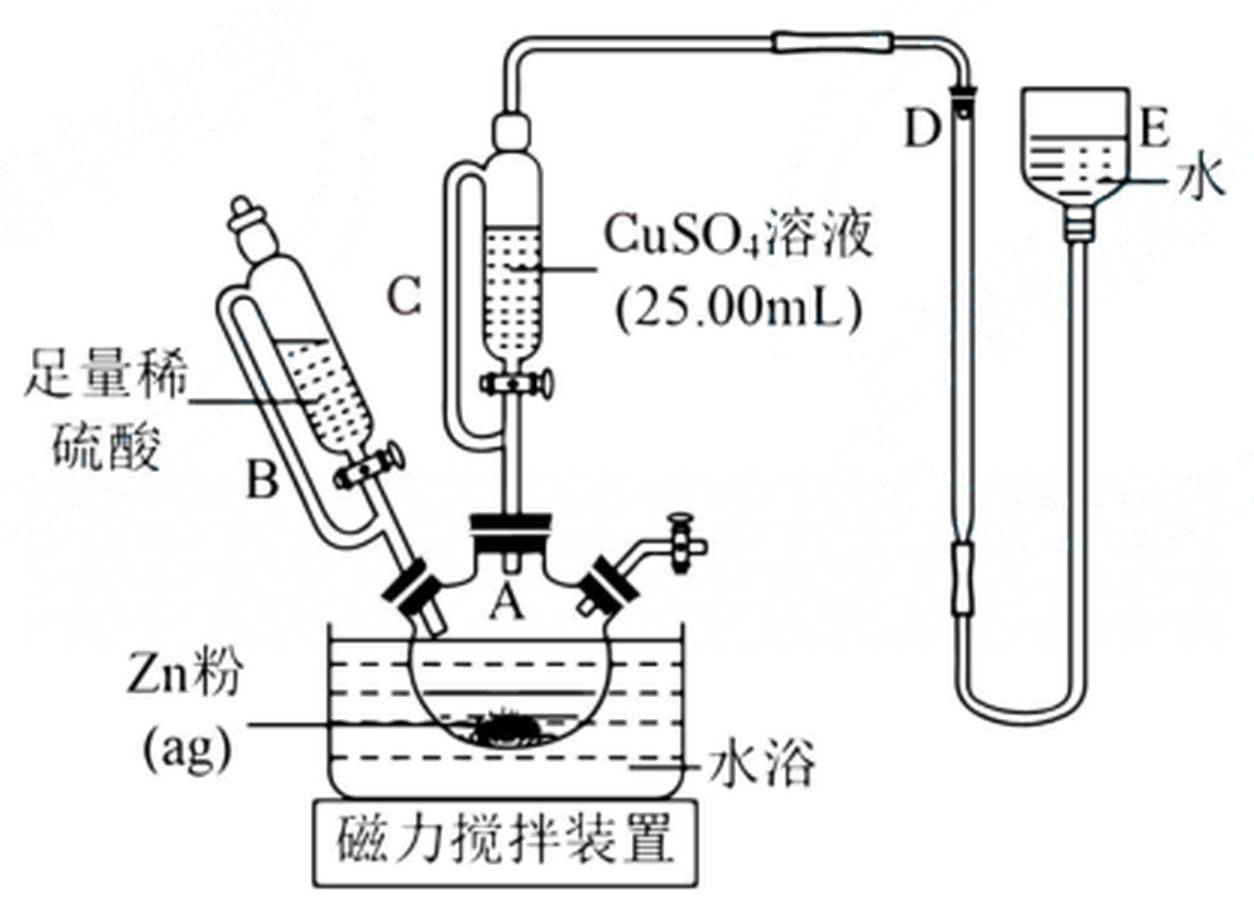
\includegraphics[width=0.46\textwidth]{figures/h2_volume_apparatus.png}
\end{center}

\begin{enumerate}[label=\textcircled{\arabic*},leftmargin=2.6em,itemsep=0.2em,topsep=0.2em]
\item 按如图安装装置（加持仪器略去）
\item ……
\item 在仪器 A、B、C、D、E 中加入如图所示的试剂
\item 调整 D、E 中两液面相平，使 D 中液面保持在 0 或略低于 0 的刻度位置，读数并记录
\item 将 \ch{CuSO4} 溶液滴入 A 中并搅拌，反应完成后，再滴加稀硫酸至体系中不再有气体产生
\item 待体系恢复到室温，移动 E 管，保持 D、E 中两液面相平，读数并记录
\item 处理数据
\end{enumerate}

\item 步骤\textcircled{2} 为\blank[8em]。

\item Zn 粉质量为 $a=0.195$ g，若测得 \ch{H2} 体积为 22.40 mL（已折算为标准状况下的体积），则\blank[8em]（写出必要的计算步骤）
\workspace[5]

\item 若步骤\textcircled{6} E 管液面高于 D 管，未调节液面即读数，则测得 $c(\mathrm{CuSO_4})=$\blank[3em]。
\choice{偏大}{偏小}{无影响}{无法判断}

\item 是否能用同样的装置和方法测定 \ch{MgSO4} 的浓度：\blank[2.6em]（填“是”或“否”）原因是\blank[6em]。

\item 如果 \ch{CuSO4} 浓度的参考值为 0.100 mol/L，而测定结果是 0.096 mol/L，则测定的相对偏差为\blank[3em]。

\item \ch{CuSO4} 溶液经过一系列操作，可以获得 $\mathrm{CuSO_4\cdot 5H_2O}$。取 2.50 g $\mathrm{CuSO_4\cdot 5H_2O}$ 受热脱水过程的热重曲线（样品质量随温度变化的曲线）如图所示。

\begin{center}
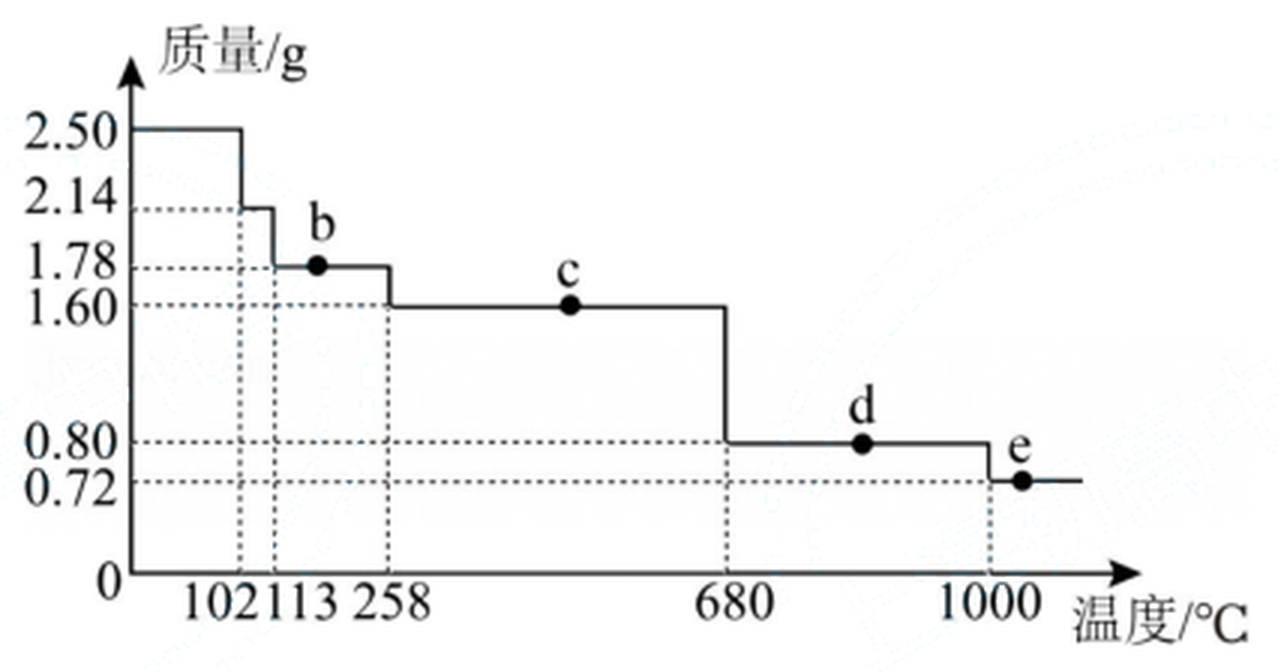
\includegraphics[width=0.48\textwidth]{figures/tga_cuso4.png}
\end{center}

请回答下列问题：b 点时固体物质的化学式\blank[5em]。

\item 取 270 ℃ 所得样品，于 770 ℃ 灼烧得到的主要产物是黑色粉末和 \ch{SO3}，该反应的化学方程式为\blank[9em]。

\item 1000 ℃ 发生反应的化学方程式为\blank[9em]。
\end{enumerate}

%==========================================================
\bigsection{五、物质的量（本题共 16 分）}

\noindent\textbf{5.（16 分）}物质的量是将微观粒子数与宏观可称量物理量联系起来的桥梁，极大地促进了化学学科的发展。

\begin{enumerate}[label=（\arabic*）]
\item 某次高空探测，收集到含 \ch{O3}、\ch{O2}、\ch{N2}（其他气体忽略不计）的大气样本，在实验室中微热一段时间后，\ch{O3} 全部转化为 \ch{O2}（$2\mathrm{O_3}=3\mathrm{O_2}$）。若气体总体积增加了 0.36\%，则大气样本中 \ch{O3} 的体积分数为\blank[3.4em]（反应前后温度和压强均保持不变）。

\item 物质 R 吸收氢气后成为 $\mathrm{RH_6}$，$\mathrm{RH_6}$ 晶体中的氢密度可达到 $1.1\times 10^{3}$ g$\cdot$m\textsuperscript{$-$3}（氢密度是指单位体积晶体中氢元素的质量），则此时 1 m\textsuperscript{3} 晶体中所储的氢相当于标准状况下\blank[5em] L 氢气。

\item 如图所示，一密闭容器被无摩擦、可自由滑动的两隔板 a、b 分成甲、乙两室；标准状况下，在乙室中充入 \ch{NH3} 0.4 mol，甲室中充入 \ch{HCl}、\ch{N2} 的混合气体，静止时隔板位置如图所示。已知甲、乙两室中气体的质量差为 17.3 g。

\begin{center}
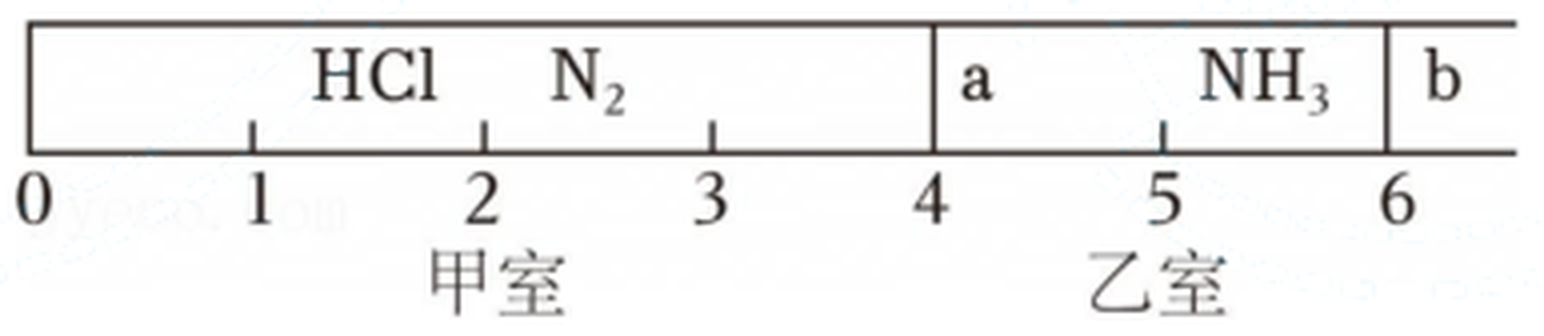
\includegraphics[width=0.62\textwidth]{figures/two_chamber_tube.png}
\end{center}

\textcircled{1} 甲室中气体总质量为\blank[3.4em] g。

\textcircled{2} 甲室中 \ch{HCl}、\ch{N2} 的物质的量之比为\blank[3em]。

\textcircled{3} 将隔板 a 去掉，当 \ch{HCl} 与 \ch{NH3} 充分反应生成 \ch{NH4Cl} 固体后（仅发生此反应），隔板 b 将位于刻度“\blank[3em]”处（填数字，不考虑固体物质产生的体积），此时体系的平均相对分子质量为\blank[3.4em]。

\item 火箭发射后，发射场附近废水中偏二甲肼（\ch{C2H8N2}）浓度变高，可用 \ch{H2O2} 对废水处理。处理 100 L 的 2000 mg/L 偏二甲肼废水，使用密度为 1.11 g/mL 30\% 的 \ch{H2O2} 溶液，则 \ch{H2O2} 溶液的理论投加量为\blank[3.4em] L（保留两位小数）。

已知：$\mathrm{C_2H_8N_2(l)+8H_2O_2(l)=N_2(g)+2CO_2(g)+12H_2O(l)}$

\item 焦亚硫酸钠（\ch{Na2S2O5}）易溶于水，与强酸反应放出较多 \ch{SO2}。\ch{Na2S2O5} 作为食品添加剂，在葡萄酒中残留量一般不得超过 0.25 g$\cdot$L\textsuperscript{$-$1}（以 \ch{SO2} 计）。小复同学检测葡萄酒样品中 \ch{Na2S2O5} 残留量，实验如下：取 150 mL 葡萄酒样品，加稀硫酸酸化后加热，将产生气体通入足量双氧水中充分吸收，再除去过量的 \ch{H2O2}，冷却后，用 0.100 mol$\cdot$L\textsuperscript{$-$1} \ch{NaOH} 溶液与上述吸收液反应，恰好反应时消耗 \ch{NaOH} 溶液 15.00 mL，则该样品中 \ch{Na2S2O5} 的残留量为\blank[4em] g$\cdot$L\textsuperscript{$-$1}（残留量以 \ch{SO2} 计）。

已知：$\mathrm{SO_2+H_2O_2=H_2SO_4}$
\workspace[6]
\end{enumerate}

%==========================================================
% 以下「参考答案」整节仅在答案版输出（试卷版由 \ifanswer 整段吞掉）
\ifanswer
\newpage
\bigsection{参考答案}

\begin{enumerate}[label=\textbf{\arabic*.},leftmargin=2.5em]
\item
\begin{enumerate}[label=（\arabic*）]
\item D；
\item $A-x+n+24$；
\item B；
\item C；
\item AD（不定项）；
\item 氚。A 为氢元素，其核素中质子数（1）为中子数（2）的一半，即 ${}_{1}^{3}\mathrm{H}$；
\item $\left[\mathrm{H}:\right]^-$（$\mathrm{H^-}$ 的电子式）；$\mathrm{Mg^{2+}}$ 的结构示意图为
\begin{center}
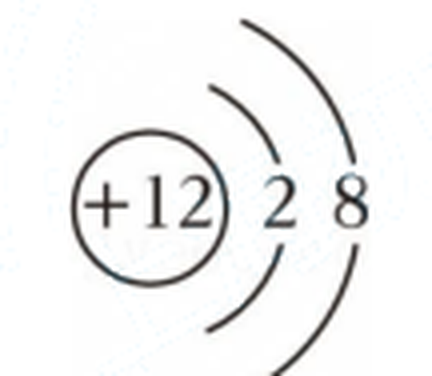
\includegraphics[width=1.1cm]{figures/mg2_plus_shell.png}
\end{center}
\item $\mathrm{SO_2+2NaOH=Na_2SO_3+H_2O}$（$EB_2$ 为 \ch{SO2}，$CBA$ 为 \ch{NaOH}）；
\item $a=7.58$，$b=49.82$；
\item AC（不定项）。
\end{enumerate}

\item
\begin{enumerate}[label=（\arabic*）]
\item D；
\item $\mathrm{FeCl_3+3H_2O}\xrightarrow{\Delta}\mathrm{Fe(OH)_3(\text{胶体})+3HCl}$；% \Delta 不可写在 \mathrm{} 内，否则映射到 Times New Roman 缺字形
\item B；
\item 阴极；电泳；
\item pH 为 $3\sim 9$ 时，溶液中的含砷微粒主要是 $\mathrm{H_2AsO_4^-}$、$\mathrm{HAsO_4^{2-}}$，\ch{Fe(OH)3} 胶体粒子带正电荷，能吸附带负电荷的 $\mathrm{H_2AsO_4^-}$、$\mathrm{HAsO_4^{2-}}$；
\item $+5$ 价；盐；
\item 向胶体中加入盐时，其中的阳离子或阴离子能中和分散质微粒所带的电荷，从而使分散质聚集成较大的微粒，在重力作用下形成沉淀析出；
\item 氨基酸通过阻碍颗粒间直接接触，增强胶体颗粒间的排斥作用来抑制胶体聚集。
\end{enumerate}

\item
\begin{enumerate}[label=（\arabic*）]
\item 蒸馏（填分离操作名称）；
\item B；
\item AD（不定项）；
\item 取少量海水于试管中，向其中加入 \ch{Ba(NO3)2} 溶液，静置，向上层清液中（或取上层清液）加入 \ch{HNO3} 酸化的 \ch{AgNO3} 溶液，若有白色沉淀生成，说明海水中有 $\mathrm{Cl^-}$；
\item 硫酸至不再产生气泡；蒸发浓缩、冷却结晶；
\item 3.8 mol$\cdot$L\textsuperscript{$-$1}（结果保留 1 位小数）；
\item \textcircled{1} 14.9 g；\textcircled{2} 胶头滴管、100 mL 容量瓶（填仪器名称）；
\item CBDBAE；
\item BC（不定项）；
\item 31.3 mL（保留 1 位小数）；
\item A。
\end{enumerate}

\item
\begin{enumerate}[label=（\arabic*）]
\item $\dfrac{40w}{233}$ mol$\cdot$L\textsuperscript{$-$1}（不用化简）；
\item 检查装置的气密性；
\item $0.08$ mol/L（写出必要的计算步骤）；
\item A；
\item 否（填“是”或“否”）；原因是 Mg 比 Zn 活泼，Zn 与 \ch{MgSO4} 不反应；
\item 4\%；
\item $\mathrm{CuSO_4\cdot H_2O}$；
\item $\mathrm{CuSO_4\xrightarrow{770\,^{\circ}\mathrm{C}}CuO+SO_3\uparrow}$；
\item $\mathrm{4CuO\xrightarrow{1000\,^{\circ}\mathrm{C}}2Cu_2O+O_2\uparrow}$。
\end{enumerate}

\item
\begin{enumerate}[label=（\arabic*）]
\item 0.72\%（反应前后温度和压强均保持不变）；
\item $1.232\times 10^{6}$ L 氢气；
\item \textcircled{1} 24.1 g；\textcircled{2} $1:3$；\textcircled{3} 4；25.25；
\item 2.72 L（保留两位小数）；
\item 0.320 g$\cdot$L\textsuperscript{$-$1}（残留量以 \ch{SO2} 计）。
\end{enumerate}
\end{enumerate}
\fi

\end{document}
"

\documentclass[11pt,a4paper]{article}
\usepackage{chem}

% ---- 卷名（页眉；答案版自动追加版本标记）----
\newcommand{\paperhead}{2025-2026 学年上海市复旦附中高一（上）月考化学试卷（10 月份）}
\fancyhead[L]{\small\kaishu \paperhead\vermark}

% ---- 标题 ----
\title{\heiti\bfseries\Large \paperhead}
\author{}
\date{}

% 原卷部分题干下方留有整段演算空白，此处预留书写空间（仅试卷版输出）
\newcommand{\workspace}[1][6]{\ansspace[#1]}

\begin{document}
\maketitle
\thispagestyle{fancy}

%==========================================================
\bigsection{一、原子结构（本题共 24 分）}

\noindent\textbf{1.（24 分）}人类对原子结构的认识是一段充满智慧的探索历程。

\begin{enumerate}[label=（\arabic*）]
\item 原子的构成及核外电子排布情况可用原子结构示意图表示，其依据是下面哪位科学家的原子结构模型\blank[2.6em]。
\choice{道尔顿}{汤姆孙}{卢瑟福}{玻尔}

\item 在 $RO_3^{n-}$ 中，共有 $x$ 个核外电子，R 原子的质量数为 $A$，则 R 原子核内含有的中子数是\blank[4em]。
\workspace[3]

\item 下列各组微粒中，具有相同质子数和电子数的一组微粒是\blank[3em]。
\choicepairs
  {$\mathrm{OH^-}$、$\mathrm{F^-}$、$\mathrm{Ne}$、$\mathrm{O^{2-}}$}
  {\ch{H2O}、\ch{CH4}、\ch{NH3}、\ch{Ne}}
  {$\mathrm{H_3O^+}$、$\mathrm{Na^+}$、$\mathrm{NH_4^+}$、$\mathrm{Mg^{2+}}$}
  {$\mathrm{O^{2-}}$、$\mathrm{F^-}$、$\mathrm{Mg^{2+}}$、$\mathrm{Al^{3+}}$}

\item 下列说法正确的是\blank[3em]。
\choicelines
  {电子在原子核外空间高速运动且能量都相等}
  {两种微粒的核外电子排布相同，则一定属于同种元素}
  {K 层上运动的电子的能量最低}
  {某原子 M 层电子数为 L 层电子数的 4 倍}

\item 锂在核工业中应用广泛，如 ${}_{3}^{6}\mathrm{Li}$ 和 ${}_{3}^{7}\mathrm{Li}$ 可作核反应堆最佳热载体，${}_{3}^{7}\mathrm{LiH}$ 和 ${}_{3}^{7}\mathrm{LiD}$ 用作高温堆减速剂。下列有关说法错误的是\blank[3em]（不定项）。
\choicepairs
  {${}_{3}^{6}\mathrm{Li}$ 和 ${}_{3}^{7}\mathrm{Li}$ 是同种核素}
  {${}_{3}^{7}\mathrm{LiH}$ 和 ${}_{3}^{7}\mathrm{LiD}$ 化学性质几乎完全相同}
  {${}_{3}^{7}\mathrm{LiH}$ 和 ${}_{3}^{7}\mathrm{LiD}$ 中质子总数相同}
  {${}_{3}^{6}\mathrm{Li}$ 和 ${}_{3}^{7}\mathrm{Li}$ 是同素异形体}
\end{enumerate}

有 A、B、C、D、E 五种元素，它们的核电荷数依次增大，且都小于 18。其中只有 C、D 为金属元素；A 和 C 的最外层均只有 1 个电子；B 和 E 的最外层电子数相同，且 B 的 L 层电子数是 K 层电子数的 3 倍；D 的最外层电子数为 E 的最外层电子数的 $\dfrac{1}{3}$。完成下列问题：

\begin{enumerate}[label=（\arabic*）,start=6]
\item A 的一种核素中质子数为中子数的一半，则该核素的名称是\blank[4em]。% 原卷作「则该核素的名称分别为______。」，其中「分别」与答案（仅一个核素「氚」）矛盾，此处删去「分别」二字，其余照原卷

\item A 形成的简单负离子的电子式为\blank[4em]；D 形成的简单正离子的结构示意图为\blank[4em]。

\item 写出少量 $EB_2$ 与 $CBA$ 溶液反应的化学方程式：\blank[8em]。

\item 硒元素的天然同位素组成如表：

\begin{center}
\begin{tabular}{|c|c|c|c|c|c|c|}
\hline
\rule{0pt}{1.3em}核素的质量数 & 74 & 76 & 77 & 78 & 80 & 82 \\
\hline
\rule{0pt}{1.3em}核素的丰度（\%） & 0.87 & 9.02 & $a$ & 23.52 & $b$ & 9.19 \\
\hline
\end{tabular}
\end{center}

已知硒元素的近似相对原子质量为 79.073，则 $a=$\blank[3.2em]，$b=$\blank[3.2em]。

\item 我国科研人员利用激光操控方法，从 Ca 原子束流中直接俘获 ${}^{41}\mathrm{Ca}$ 原子，实现了对同位素 ${}^{41}\mathrm{Ca}$ 的灵敏检测。${}^{41}\mathrm{Ca}$ 的半衰期（放射性元素的原子核有半数发生衰变所需的时间）长达 10 万年，是 ${}^{14}\mathrm{C}$ 的 17 倍，可应用于地球科学与考古学。下列说法正确的是\blank[3em]（不定项）。

\begin{center}
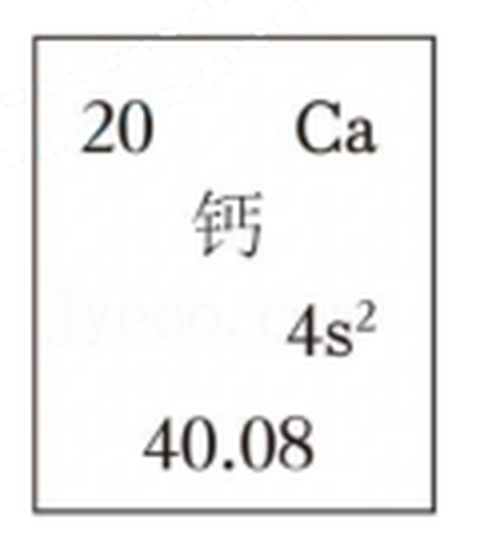
\includegraphics[width=1.7cm]{figures/ca_element_box.png}
\end{center}

\choicepairs
  {如图中 40.08 指钙元素的相对原子质量}
  {${}^{41}\mathrm{Ca}$ 的半衰期长，说明 ${}^{41}\mathrm{Ca}$ 难以失去电子}
  {${}^{41}\mathrm{Ca}$ 的衰变速度小于 ${}^{14}\mathrm{C}$ 的衰变速度}
  {从 Ca 原子束流中直接俘获 ${}^{41}\mathrm{Ca}$ 原子的过程属于化学变化}
\end{enumerate}

%==========================================================
\bigsection{二、胶体化学（本题共 16 分）}

\noindent\textbf{2.（16 分）}胶体在生命科学、材料科学及环境科学中具有广泛应用。近年来，各向异性胶体组装、生物大分子稳定性等研究为胶体化学开辟了新方向。

\begin{enumerate}[label=（\arabic*）]
\item 下列有关胶体的叙述中，正确的是\blank[3em]。
\choicelines
  {胶体区别于溶液的本质特征是胶体能够产生丁达尔现象}
  {将饱和 \ch{FeCl3} 溶液直接加热煮沸可制得 \ch{Fe(OH)3} 胶体}
  {不断搅拌后，\ch{Fe(OH)3} 胶体仍然能够稳定存在}
  {明矾[$\mathrm{KAl(SO_4)_2\cdot 12H_2O}$]可用于净水是利用了胶体粒子具有较好的吸附性}

\item 复核实验小组设计不同的实验对其制得的 \ch{Fe(OH)3} 胶体进行性质探究。写出制备 \ch{Fe(OH)3} 胶体的化学方程式：\blank[9em]。

\item 提纯制得的 \ch{Fe(OH)3} 胶体的装置是如图中的\blank[2.6em]。

\begin{center}
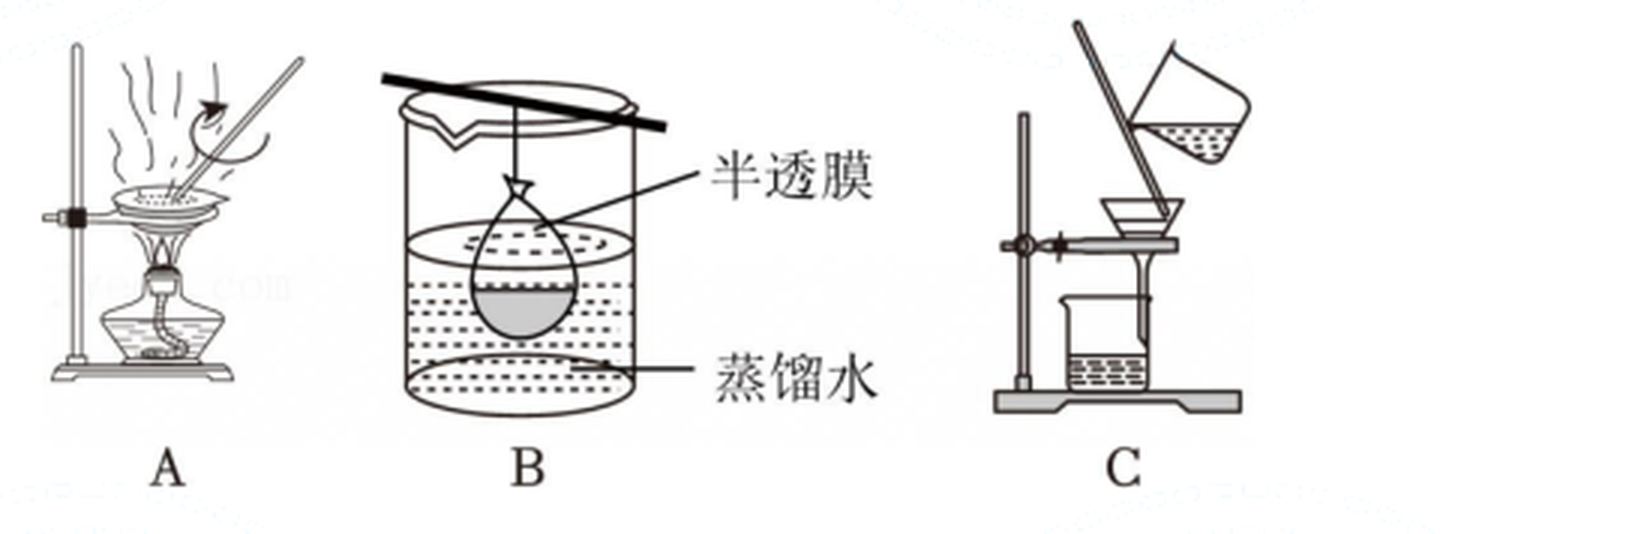
\includegraphics[width=0.80\textwidth]{figures/feoh3_purify.png}
\end{center}

\item 将提纯后的 \ch{Fe(OH)3} 胶体置于 U 形管中，通直流电一段时间后，观察到\blank[2.8em]（填“阳极”或“阴极”）附近红褐色加深，该现象称为\blank[3.4em]。

研究表明，\ch{Fe(OH)3} 胶体可净化水中低浓度的砷酸（\ch{H3AsO4}）。如图所示是不同 pH 时 \ch{Fe(OH)3} 胶体对低浓度砷酸的吸附效率曲线。

\begin{center}
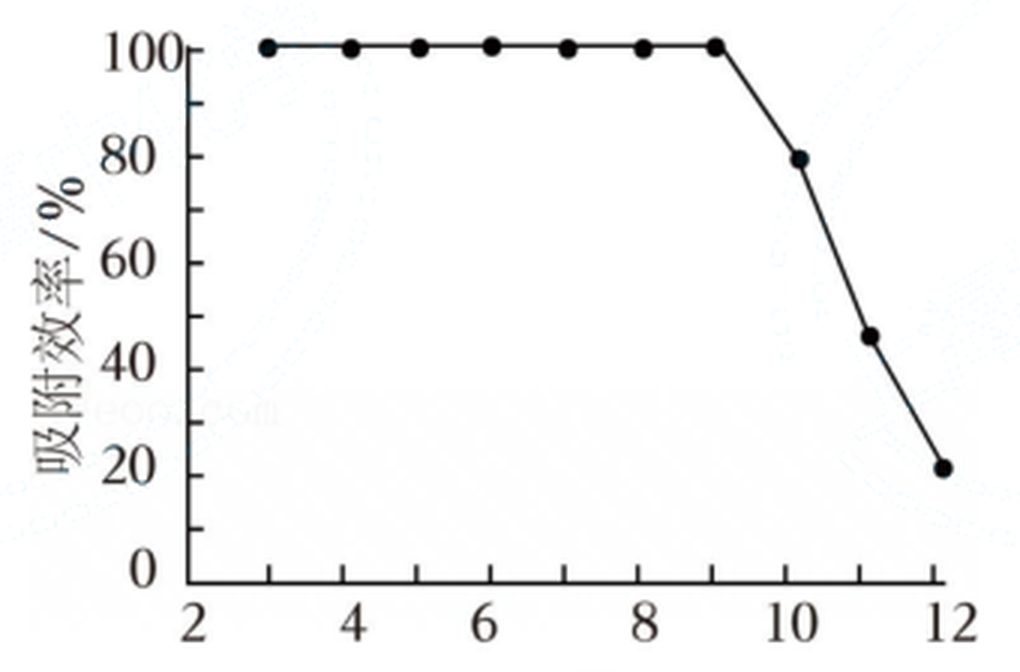
\includegraphics[width=0.42\textwidth]{figures/as_adsorption_ph.png}
\end{center}

已知：pH 反映溶液的酸碱性，pH 越高，溶液的碱性越强。pH 为 $3\sim 9$ 时，溶液中的含砷微粒主要是 $\mathrm{H_2AsO_4^-}$、$\mathrm{HAsO_4^{2-}}$。

\item pH 为 $3\sim 9$ 时，\ch{Fe(OH)3} 胶体对砷酸的吸附效率较高，其可能的原因是\blank[8em]。

\item 当水中砷酸浓度较高时，\ch{Fe(OH)3} 胶体将直接与砷酸发生化学反应生成砷酸铁（\ch{FeAsO4}）沉淀，其中砷元素是\blank[2.6em]价。$\mathrm{AsO_4^{3-}}$ 是酸根离子，则 \ch{FeAsO4} 属于\blank[3em]（填“酸”“碱”“盐”或“氧化物”）。

\item 2025 年《Nature》刊载了南方科技大学罗智团队关于氨基酸稳定胶体机制的研究。该研究发现，氨基酸（如脯氨酸、甘氨酸等）可作为稳定剂，通过吸引屏蔽机制，可逆地吸附在蛋白质、DNA 或纳米颗粒等胶体粒子的特定表面位点，削弱胶体粒子间的吸引力，从而显著提升胶体分散系的稳定性。这与电解质（如 \ch{NaCl}、\ch{Na2SO4} 等）促使胶体聚沉的作用机制相反。电解质（如 \ch{NaCl}、\ch{Na2SO4} 等）促使胶体聚沉的作用机制是\blank[8em]。

\item 蛋白药物制剂属于胶体分散系，其常常因蛋白质的相互聚集而失去药效。为了延长药物的有效期，免疫球蛋白制剂（如 Cuvitru\textsuperscript{\textregistered}）中常添加脯氨酸和甘氨酸。根据上述研究，阐述其延长有效期的主要原理是\blank[8em]。
\end{enumerate}

%==========================================================
\bigsection{三、海洋资源（本题共 25 分）}

\noindent\textbf{3.（25 分）}海洋是一座资源的宝库，化学工业中的许多基础原料都来自海洋。

\begin{enumerate}[label=（\arabic*）]
\item 海水淡化可缓解淡水资源匮乏问题。如图为太阳能海水淡化装置，该装置利用的原理是\blank[3.8em]（填分离操作名称）。

\begin{center}
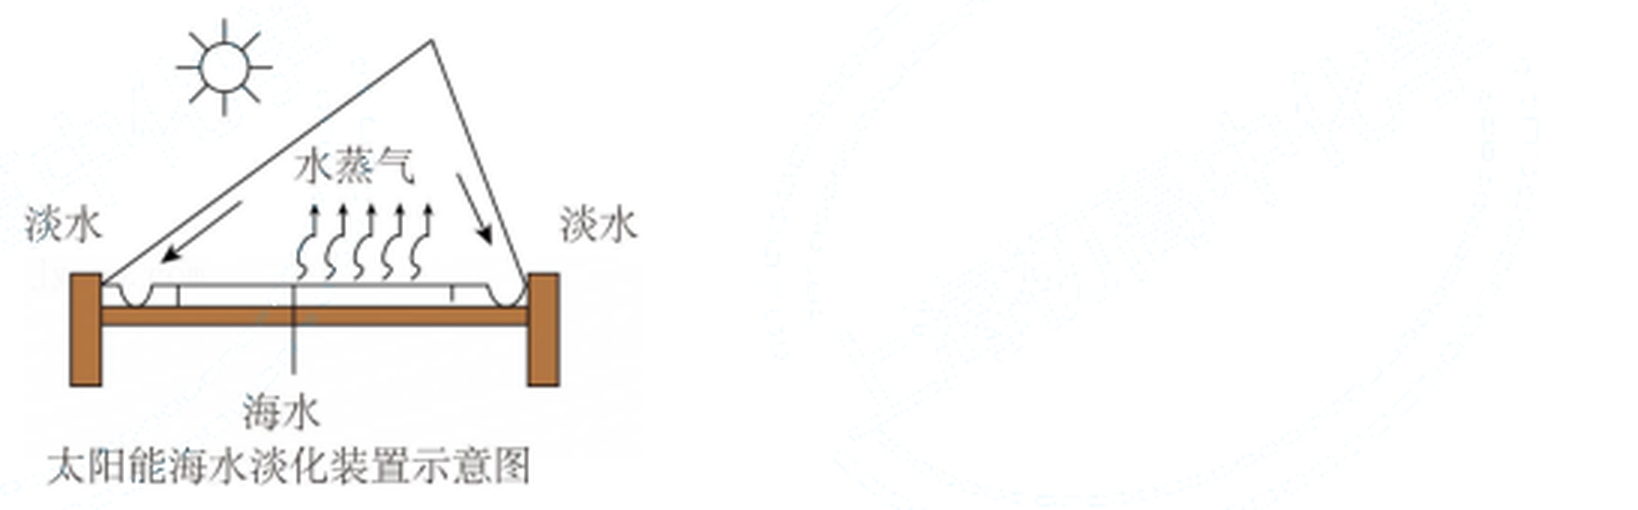
\includegraphics[width=0.52\textwidth]{figures/solar_desalination.png}
\end{center}

\item 利用海洋资源海带可以提取碘。实验室采用“萃取分液”的方法分离碘单质与有机溶剂。以下相关操作错误的是\blank[2.6em]。
% 注：该四联图中的第四个标签原卷即误印为「B.分液」（应为 D.分液），此处照原卷保留，未作改动。

\begin{center}
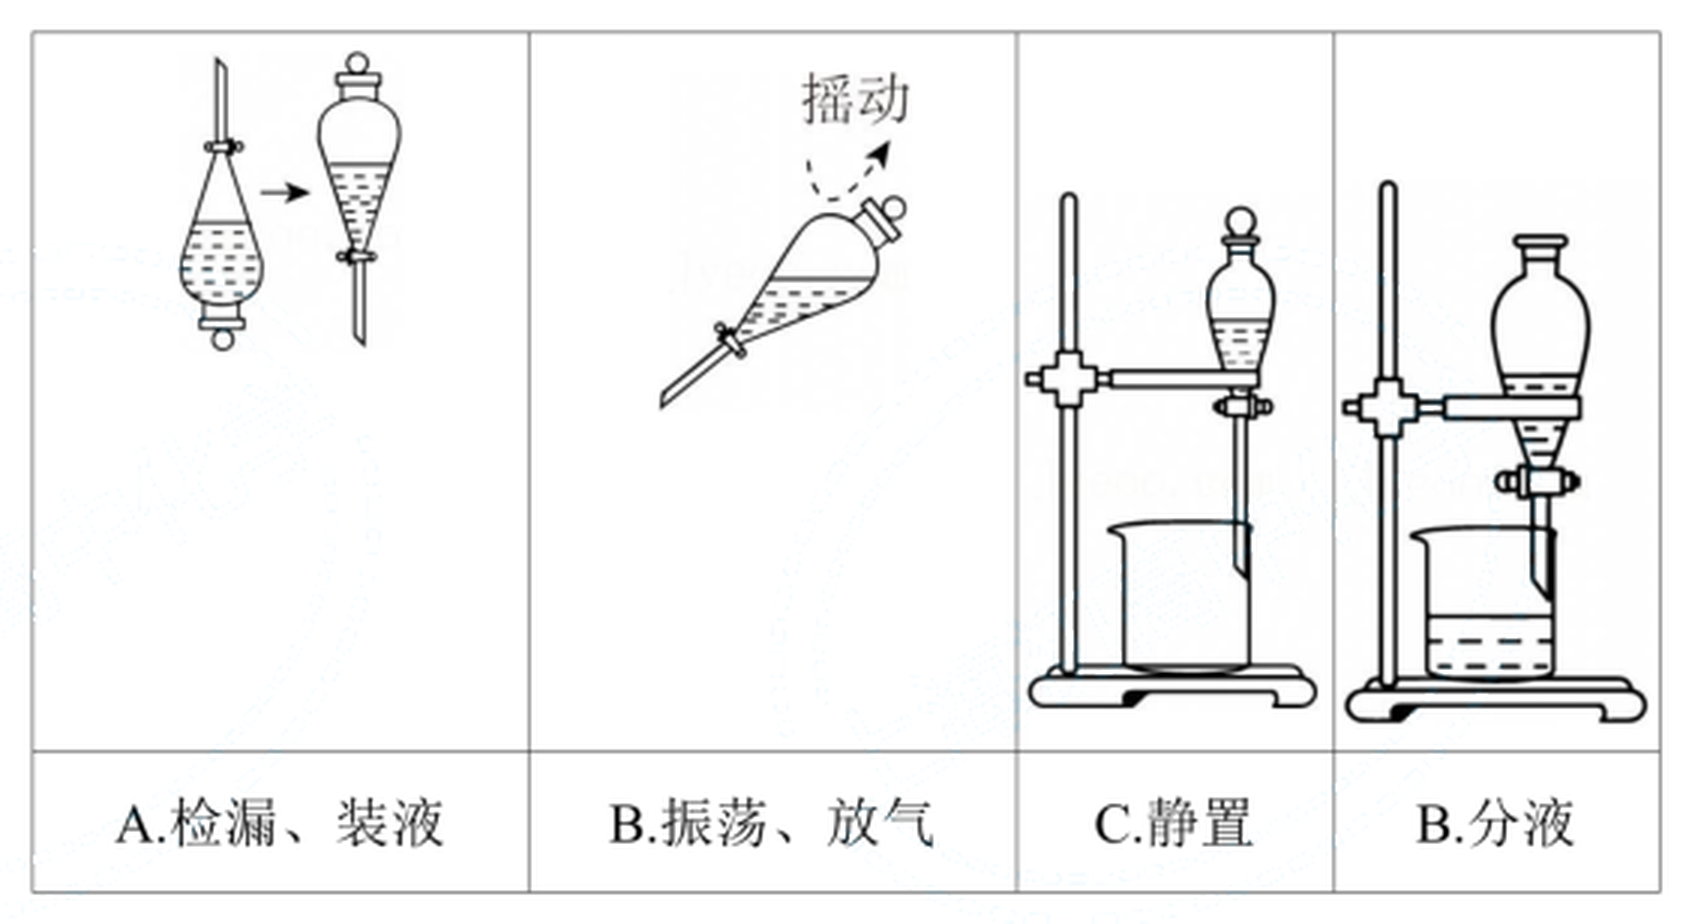
\includegraphics[width=0.68\textwidth]{figures/iodine_extraction.png}
\end{center}

\item 萃取碘水中的碘单质，可以选择的萃取剂种类很多，但不包括\blank[3em]（不定项）。
\choice{酒精}{四氯化碳}{苯}{\ch{NaCl} 溶液}

$\mathrm{SO_4^{2-}}$ 是海洋中硫元素的主要存在形式之一，其存在会干扰海水中 $\mathrm{Cl^-}$ 的检验。

\item 检验海水中 $\mathrm{Cl^-}$ 的方法是\blank[10em]。

\item 某 \ch{Na2SO4} 溶液中含有少量 \ch{Na2CO3}，已知 \ch{Na2SO4} 和 \ch{Na2CO3} 的溶解度曲线如图所示，则从该溶液中获得 $\mathrm{Na_2SO_4\cdot 10H_2O}$ 的操作是加入\blank[5em]后，\blank[4em]、\blank[4em]、过滤、洗涤、干燥。

\begin{center}
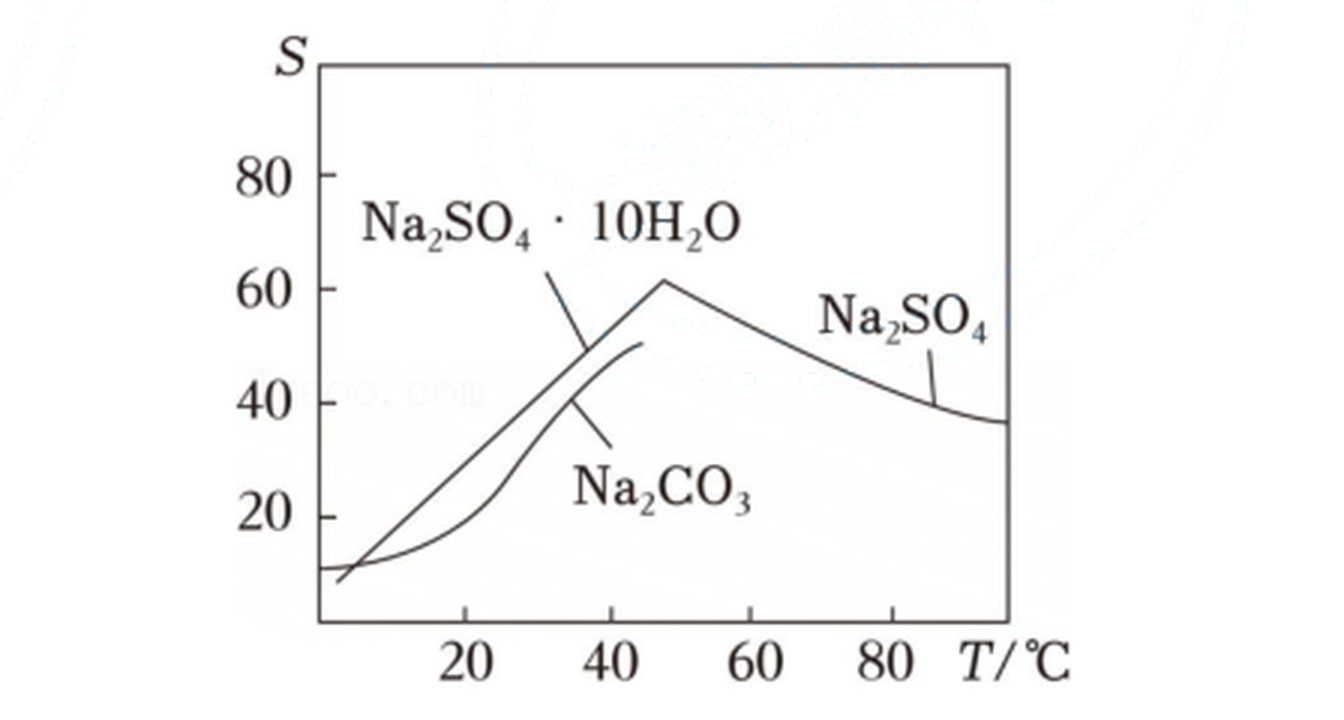
\includegraphics[width=0.48\textwidth]{figures/solubility_na2so4.png}
\end{center}

\item 以海水为原料可制取“84”消毒液。如图所示为某市售“84”消毒液标签上的部分数据，请回答下列问题。

\begin{center}
\begin{tabular}{|l|}
\hline
\rule{0pt}{1.3em}【有效成分】\ch{NaClO} \\
\hline
\rule{0pt}{1.3em}【质量分数】24\% \\
\hline
\rule{0pt}{1.3em}【溶液密度】1.18 g/cm\textsuperscript{3} \\
\hline
\rule{0pt}{1.3em}【净含量】1000 mL \\
\hline
\end{tabular}
\end{center}

该“84”消毒液的物质的量浓度约为\blank[3.4em] mol$\cdot$L\textsuperscript{$-$1}（结果保留 1 位小数）。

\item \textcircled{1} 欲配制 80 mL 2.000 mol$\cdot$L\textsuperscript{$-$1} \ch{NaClO} 溶液，需准确称量 \ch{NaClO} 固体\blank[3.4em] g。

\textcircled{2} 配制该溶液过程中所用玻璃仪器有烧杯、玻璃棒、\blank[6em]（填仪器名称）。

\item 如图是配制溶液的几个关键实验步骤和操作。

\begin{center}
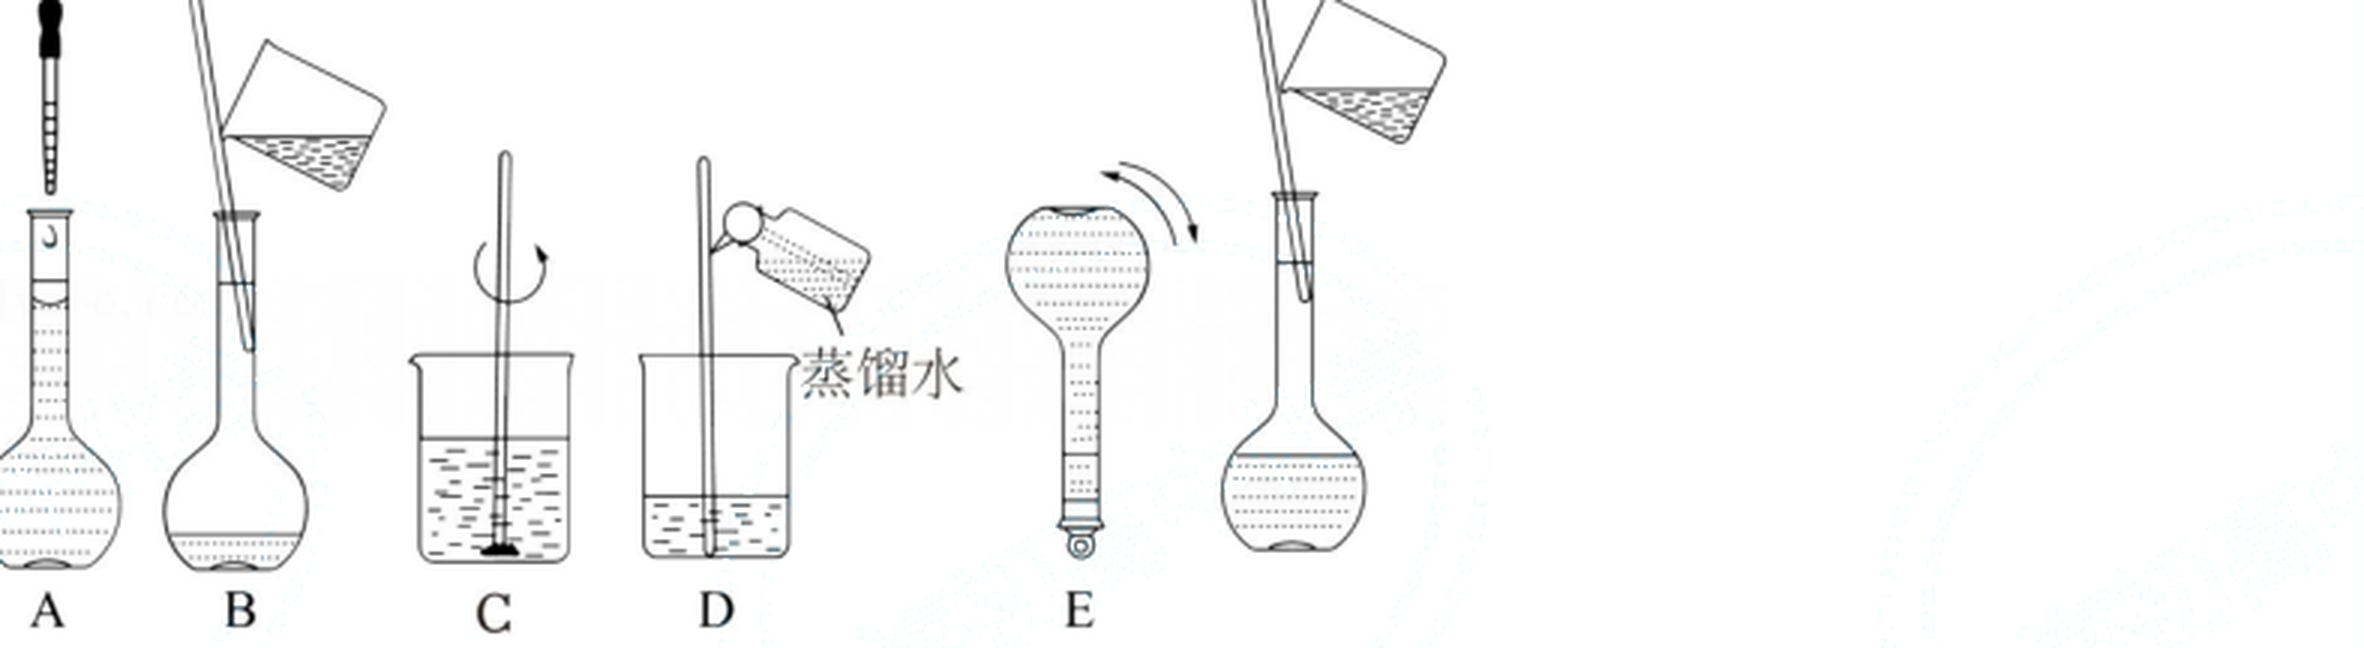
\includegraphics[width=0.88\textwidth]{figures/dilution_steps.png}
\end{center}

将上述实验步骤 A$\sim$E 按实验过程先后次序排列\blank[6em]。

\item 若所配制的次氯酸钠溶液浓度偏低，原因可能是\blank[3em]（不定项）。
\choicelines
  {配制前，容量瓶中有少量蒸馏水}
  {洗涤液未转移到容量瓶中}
  {定容时，仰视刻度线}
  {定容摇匀后，有少量溶液外流}

\item “84”消毒液与稀硫酸混合使用可增强消毒能力，某消毒小组人员用 98\%（密度为 1.84 g$\cdot$cm\textsuperscript{$-$3}）的浓硫酸配制 250 mL 2.3 mol$\cdot$L\textsuperscript{$-$1} 的稀硫酸用于增强“84”消毒液的消毒能力。需要浓硫酸的体积为\blank[3.4em] mL（保留 1 位小数）。

\item 若在用浓硫酸配制稀硫酸时，将量筒、烧杯、玻璃棒均洗涤 $2\sim 3$ 次，并将洗涤液转入容量瓶，会造成所配制的稀硫酸的浓度\blank[2.6em]。
\choicethree{偏高}{偏低}{无影响}
\end{enumerate}

%==========================================================
\bigsection{四、\ch{CuSO4} 溶液（本题共 19 分）}

\noindent\textbf{4.（19 分）}旦旦实验小组为测定 \ch{CuSO4} 溶液的浓度，设计了两个方案。

\noindentⅠ. 甲方案：取 25 mL \ch{CuSO4} 溶液，加入足量 \ch{BaCl2} 溶液，待沉淀完全后，经过滤、洗涤、干燥，得到干燥纯净的 \ch{BaSO4}，称量。

\begin{enumerate}[label=（\arabic*）]
\item 若固体质量为 $w$ g，则 $c(\mathrm{CuSO_4})=$\blank[7em] mol$\cdot$L\textsuperscript{$-$1}（不用化简）。

\item[] \noindentⅡ. 乙方案。实验步骤：

\begin{center}
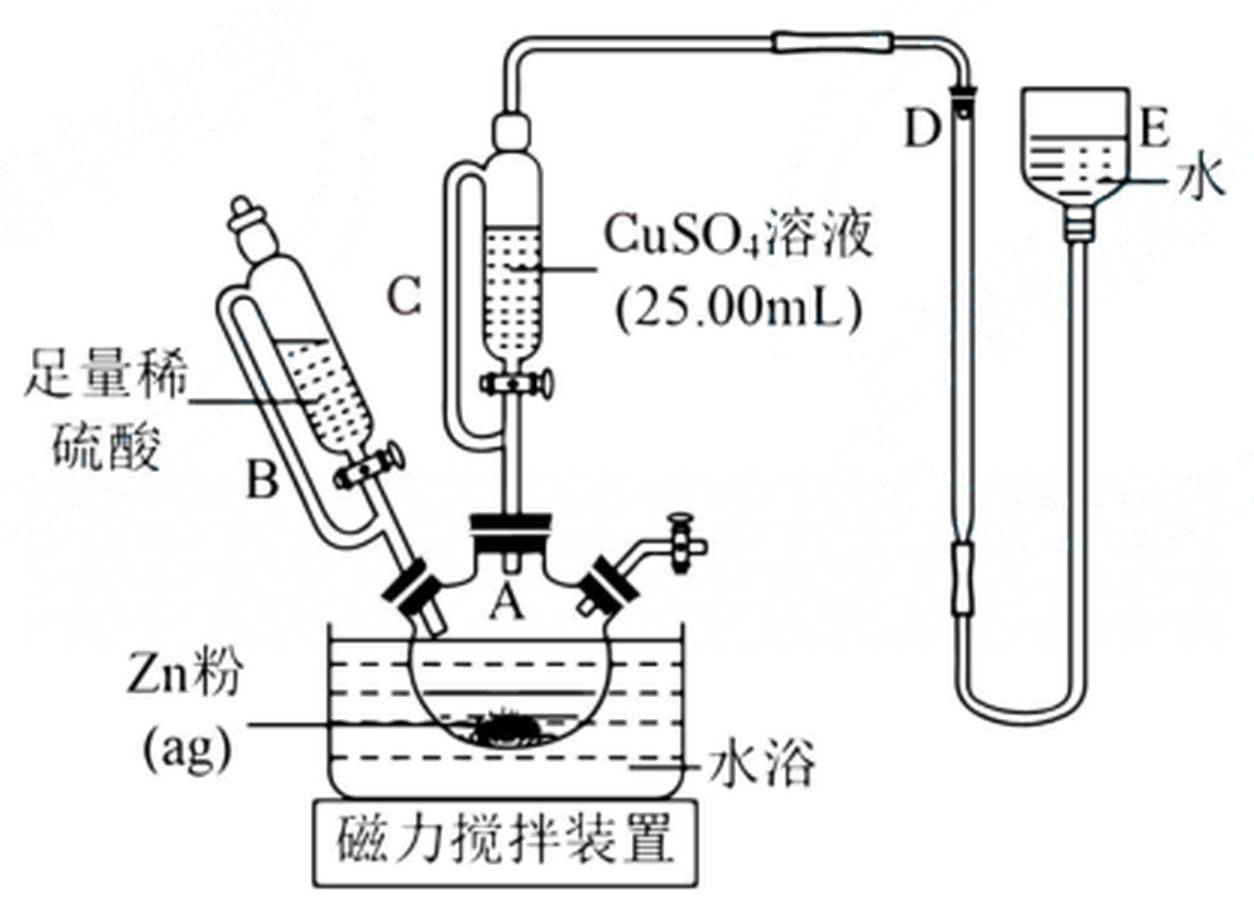
\includegraphics[width=0.46\textwidth]{figures/h2_volume_apparatus.png}
\end{center}

\begin{enumerate}[label=\textcircled{\arabic*},leftmargin=2.6em,itemsep=0.2em,topsep=0.2em]
\item 按如图安装装置（加持仪器略去）
\item ……
\item 在仪器 A、B、C、D、E 中加入如图所示的试剂
\item 调整 D、E 中两液面相平，使 D 中液面保持在 0 或略低于 0 的刻度位置，读数并记录
\item 将 \ch{CuSO4} 溶液滴入 A 中并搅拌，反应完成后，再滴加稀硫酸至体系中不再有气体产生
\item 待体系恢复到室温，移动 E 管，保持 D、E 中两液面相平，读数并记录
\item 处理数据
\end{enumerate}

\item 步骤\textcircled{2} 为\blank[8em]。

\item Zn 粉质量为 $a=0.195$ g，若测得 \ch{H2} 体积为 22.40 mL（已折算为标准状况下的体积），则\blank[8em]（写出必要的计算步骤）
\workspace[5]

\item 若步骤\textcircled{6} E 管液面高于 D 管，未调节液面即读数，则测得 $c(\mathrm{CuSO_4})=$\blank[3em]。
\choice{偏大}{偏小}{无影响}{无法判断}

\item 是否能用同样的装置和方法测定 \ch{MgSO4} 的浓度：\blank[2.6em]（填“是”或“否”）原因是\blank[6em]。

\item 如果 \ch{CuSO4} 浓度的参考值为 0.100 mol/L，而测定结果是 0.096 mol/L，则测定的相对偏差为\blank[3em]。

\item \ch{CuSO4} 溶液经过一系列操作，可以获得 $\mathrm{CuSO_4\cdot 5H_2O}$。取 2.50 g $\mathrm{CuSO_4\cdot 5H_2O}$ 受热脱水过程的热重曲线（样品质量随温度变化的曲线）如图所示。

\begin{center}
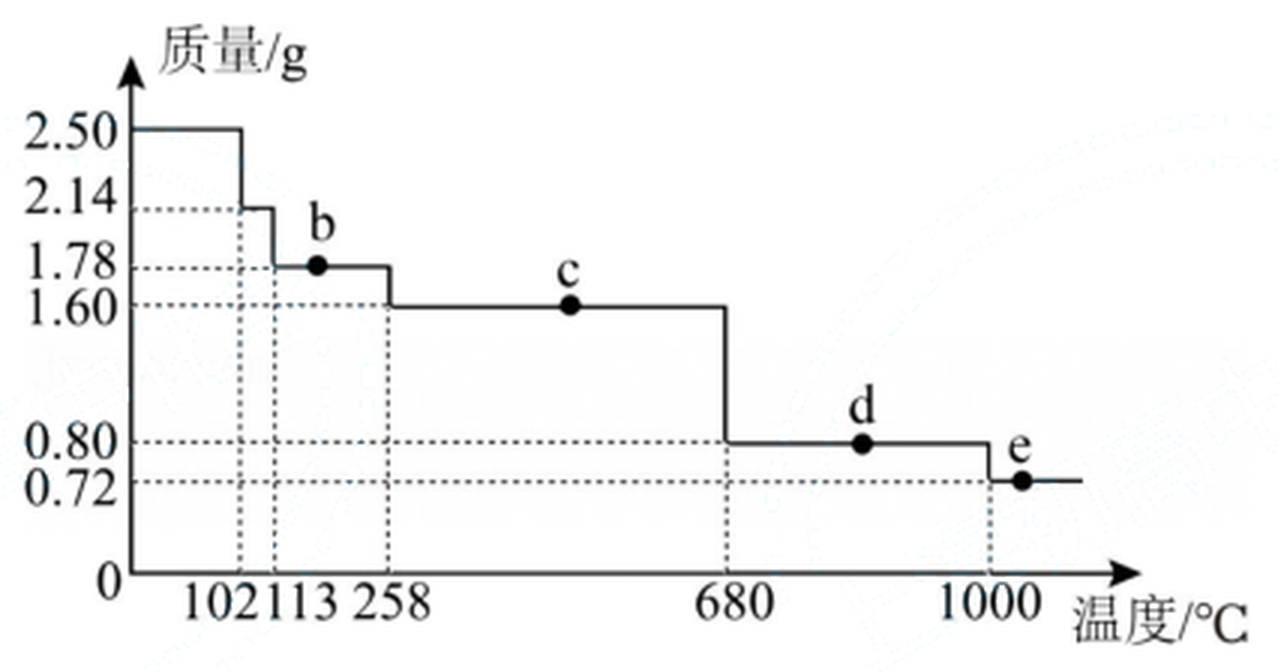
\includegraphics[width=0.48\textwidth]{figures/tga_cuso4.png}
\end{center}

请回答下列问题：b 点时固体物质的化学式\blank[5em]。

\item 取 270 ℃ 所得样品，于 770 ℃ 灼烧得到的主要产物是黑色粉末和 \ch{SO3}，该反应的化学方程式为\blank[9em]。

\item 1000 ℃ 发生反应的化学方程式为\blank[9em]。
\end{enumerate}

%==========================================================
\bigsection{五、物质的量（本题共 16 分）}

\noindent\textbf{5.（16 分）}物质的量是将微观粒子数与宏观可称量物理量联系起来的桥梁，极大地促进了化学学科的发展。

\begin{enumerate}[label=（\arabic*）]
\item 某次高空探测，收集到含 \ch{O3}、\ch{O2}、\ch{N2}（其他气体忽略不计）的大气样本，在实验室中微热一段时间后，\ch{O3} 全部转化为 \ch{O2}（$2\mathrm{O_3}=3\mathrm{O_2}$）。若气体总体积增加了 0.36\%，则大气样本中 \ch{O3} 的体积分数为\blank[3.4em]（反应前后温度和压强均保持不变）。

\item 物质 R 吸收氢气后成为 $\mathrm{RH_6}$，$\mathrm{RH_6}$ 晶体中的氢密度可达到 $1.1\times 10^{3}$ g$\cdot$m\textsuperscript{$-$3}（氢密度是指单位体积晶体中氢元素的质量），则此时 1 m\textsuperscript{3} 晶体中所储的氢相当于标准状况下\blank[5em] L 氢气。

\item 如图所示，一密闭容器被无摩擦、可自由滑动的两隔板 a、b 分成甲、乙两室；标准状况下，在乙室中充入 \ch{NH3} 0.4 mol，甲室中充入 \ch{HCl}、\ch{N2} 的混合气体，静止时隔板位置如图所示。已知甲、乙两室中气体的质量差为 17.3 g。

\begin{center}
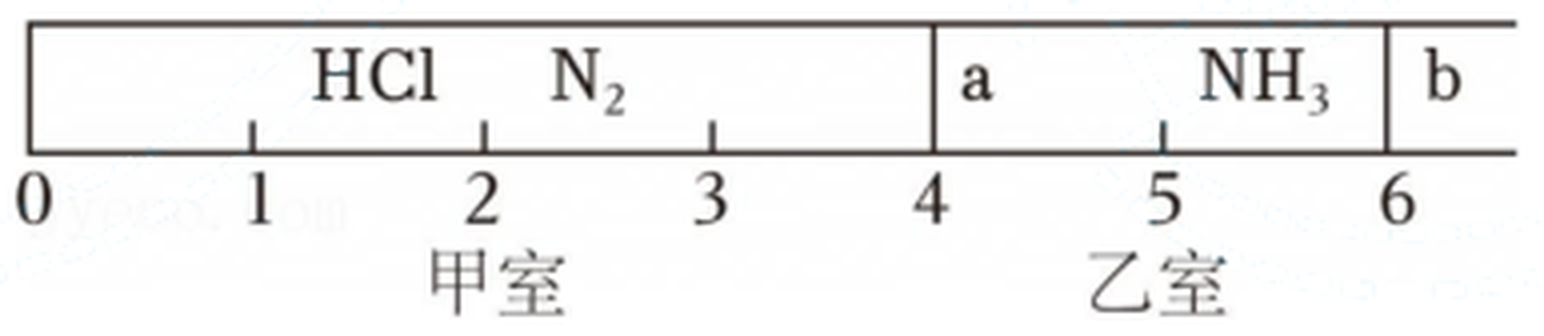
\includegraphics[width=0.62\textwidth]{figures/two_chamber_tube.png}
\end{center}

\textcircled{1} 甲室中气体总质量为\blank[3.4em] g。

\textcircled{2} 甲室中 \ch{HCl}、\ch{N2} 的物质的量之比为\blank[3em]。

\textcircled{3} 将隔板 a 去掉，当 \ch{HCl} 与 \ch{NH3} 充分反应生成 \ch{NH4Cl} 固体后（仅发生此反应），隔板 b 将位于刻度“\blank[3em]”处（填数字，不考虑固体物质产生的体积），此时体系的平均相对分子质量为\blank[3.4em]。

\item 火箭发射后，发射场附近废水中偏二甲肼（\ch{C2H8N2}）浓度变高，可用 \ch{H2O2} 对废水处理。处理 100 L 的 2000 mg/L 偏二甲肼废水，使用密度为 1.11 g/mL 30\% 的 \ch{H2O2} 溶液，则 \ch{H2O2} 溶液的理论投加量为\blank[3.4em] L（保留两位小数）。

已知：$\mathrm{C_2H_8N_2(l)+8H_2O_2(l)=N_2(g)+2CO_2(g)+12H_2O(l)}$

\item 焦亚硫酸钠（\ch{Na2S2O5}）易溶于水，与强酸反应放出较多 \ch{SO2}。\ch{Na2S2O5} 作为食品添加剂，在葡萄酒中残留量一般不得超过 0.25 g$\cdot$L\textsuperscript{$-$1}（以 \ch{SO2} 计）。小复同学检测葡萄酒样品中 \ch{Na2S2O5} 残留量，实验如下：取 150 mL 葡萄酒样品，加稀硫酸酸化后加热，将产生气体通入足量双氧水中充分吸收，再除去过量的 \ch{H2O2}，冷却后，用 0.100 mol$\cdot$L\textsuperscript{$-$1} \ch{NaOH} 溶液与上述吸收液反应，恰好反应时消耗 \ch{NaOH} 溶液 15.00 mL，则该样品中 \ch{Na2S2O5} 的残留量为\blank[4em] g$\cdot$L\textsuperscript{$-$1}（残留量以 \ch{SO2} 计）。

已知：$\mathrm{SO_2+H_2O_2=H_2SO_4}$
\workspace[6]
\end{enumerate}

%==========================================================
% 以下「参考答案」整节仅在答案版输出（试卷版由 \ifanswer 整段吞掉）
\ifanswer
\newpage
\bigsection{参考答案}

\begin{enumerate}[label=\textbf{\arabic*.},leftmargin=2.5em]
\item
\begin{enumerate}[label=（\arabic*）]
\item D；
\item $A-x+n+24$；
\item B；
\item C；
\item AD（不定项）；
\item 氚。A 为氢元素，其核素中质子数（1）为中子数（2）的一半，即 ${}_{1}^{3}\mathrm{H}$；
\item $\left[\mathrm{H}:\right]^-$（$\mathrm{H^-}$ 的电子式）；$\mathrm{Mg^{2+}}$ 的结构示意图为
\begin{center}
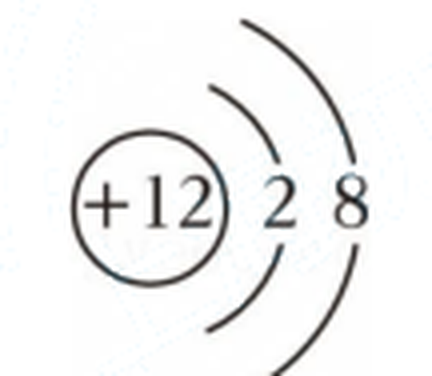
\includegraphics[width=1.1cm]{figures/mg2_plus_shell.png}
\end{center}
\item $\mathrm{SO_2+2NaOH=Na_2SO_3+H_2O}$（$EB_2$ 为 \ch{SO2}，$CBA$ 为 \ch{NaOH}）；
\item $a=7.58$，$b=49.82$；
\item AC（不定项）。
\end{enumerate}

\item
\begin{enumerate}[label=（\arabic*）]
\item D；
\item $\mathrm{FeCl_3+3H_2O}\xrightarrow{\Delta}\mathrm{Fe(OH)_3(\text{胶体})+3HCl}$；% \Delta 不可写在 \mathrm{} 内，否则映射到 Times New Roman 缺字形
\item B；
\item 阴极；电泳；
\item pH 为 $3\sim 9$ 时，溶液中的含砷微粒主要是 $\mathrm{H_2AsO_4^-}$、$\mathrm{HAsO_4^{2-}}$，\ch{Fe(OH)3} 胶体粒子带正电荷，能吸附带负电荷的 $\mathrm{H_2AsO_4^-}$、$\mathrm{HAsO_4^{2-}}$；
\item $+5$ 价；盐；
\item 向胶体中加入盐时，其中的阳离子或阴离子能中和分散质微粒所带的电荷，从而使分散质聚集成较大的微粒，在重力作用下形成沉淀析出；
\item 氨基酸通过阻碍颗粒间直接接触，增强胶体颗粒间的排斥作用来抑制胶体聚集。
\end{enumerate}

\item
\begin{enumerate}[label=（\arabic*）]
\item 蒸馏（填分离操作名称）；
\item B；
\item AD（不定项）；
\item 取少量海水于试管中，向其中加入 \ch{Ba(NO3)2} 溶液，静置，向上层清液中（或取上层清液）加入 \ch{HNO3} 酸化的 \ch{AgNO3} 溶液，若有白色沉淀生成，说明海水中有 $\mathrm{Cl^-}$；
\item 硫酸至不再产生气泡；蒸发浓缩、冷却结晶；
\item 3.8 mol$\cdot$L\textsuperscript{$-$1}（结果保留 1 位小数）；
\item \textcircled{1} 14.9 g；\textcircled{2} 胶头滴管、100 mL 容量瓶（填仪器名称）；
\item CBDBAE；
\item BC（不定项）；
\item 31.3 mL（保留 1 位小数）；
\item A。
\end{enumerate}

\item
\begin{enumerate}[label=（\arabic*）]
\item $\dfrac{40w}{233}$ mol$\cdot$L\textsuperscript{$-$1}（不用化简）；
\item 检查装置的气密性；
\item $0.08$ mol/L（写出必要的计算步骤）；
\item A；
\item 否（填“是”或“否”）；原因是 Mg 比 Zn 活泼，Zn 与 \ch{MgSO4} 不反应；
\item 4\%；
\item $\mathrm{CuSO_4\cdot H_2O}$；
\item $\mathrm{CuSO_4\xrightarrow{770\,^{\circ}\mathrm{C}}CuO+SO_3\uparrow}$；
\item $\mathrm{4CuO\xrightarrow{1000\,^{\circ}\mathrm{C}}2Cu_2O+O_2\uparrow}$。
\end{enumerate}

\item
\begin{enumerate}[label=（\arabic*）]
\item 0.72\%（反应前后温度和压强均保持不变）；
\item $1.232\times 10^{6}$ L 氢气；
\item \textcircled{1} 24.1 g；\textcircled{2} $1:3$；\textcircled{3} 4；25.25；
\item 2.72 L（保留两位小数）；
\item 0.320 g$\cdot$L\textsuperscript{$-$1}（残留量以 \ch{SO2} 计）。
\end{enumerate}
\end{enumerate}
\fi

\end{document}
"

\documentclass[11pt,a4paper]{article}
\usepackage{chem}

% ---- 卷名（页眉；答案版自动追加版本标记）----
\newcommand{\paperhead}{2025-2026 学年上海市复旦附中高一（上）月考化学试卷（10 月份）}
\fancyhead[L]{\small\kaishu \paperhead\vermark}

% ---- 标题 ----
\title{\heiti\bfseries\Large \paperhead}
\author{}
\date{}

% 原卷部分题干下方留有整段演算空白，此处预留书写空间（仅试卷版输出）
\newcommand{\workspace}[1][6]{\ansspace[#1]}

\begin{document}
\maketitle
\thispagestyle{fancy}

%==========================================================
\bigsection{一、原子结构（本题共 24 分）}

\noindent\textbf{1.（24 分）}人类对原子结构的认识是一段充满智慧的探索历程。

\begin{enumerate}[label=（\arabic*）]
\item 原子的构成及核外电子排布情况可用原子结构示意图表示，其依据是下面哪位科学家的原子结构模型\blank[2.6em]。
\choice{道尔顿}{汤姆孙}{卢瑟福}{玻尔}

\item 在 $RO_3^{n-}$ 中，共有 $x$ 个核外电子，R 原子的质量数为 $A$，则 R 原子核内含有的中子数是\blank[4em]。
\workspace[3]

\item 下列各组微粒中，具有相同质子数和电子数的一组微粒是\blank[3em]。
\choicepairs
  {$\mathrm{OH^-}$、$\mathrm{F^-}$、$\mathrm{Ne}$、$\mathrm{O^{2-}}$}
  {\ch{H2O}、\ch{CH4}、\ch{NH3}、\ch{Ne}}
  {$\mathrm{H_3O^+}$、$\mathrm{Na^+}$、$\mathrm{NH_4^+}$、$\mathrm{Mg^{2+}}$}
  {$\mathrm{O^{2-}}$、$\mathrm{F^-}$、$\mathrm{Mg^{2+}}$、$\mathrm{Al^{3+}}$}

\item 下列说法正确的是\blank[3em]。
\choicelines
  {电子在原子核外空间高速运动且能量都相等}
  {两种微粒的核外电子排布相同，则一定属于同种元素}
  {K 层上运动的电子的能量最低}
  {某原子 M 层电子数为 L 层电子数的 4 倍}

\item 锂在核工业中应用广泛，如 ${}_{3}^{6}\mathrm{Li}$ 和 ${}_{3}^{7}\mathrm{Li}$ 可作核反应堆最佳热载体，${}_{3}^{7}\mathrm{LiH}$ 和 ${}_{3}^{7}\mathrm{LiD}$ 用作高温堆减速剂。下列有关说法错误的是\blank[3em]（不定项）。
\choicepairs
  {${}_{3}^{6}\mathrm{Li}$ 和 ${}_{3}^{7}\mathrm{Li}$ 是同种核素}
  {${}_{3}^{7}\mathrm{LiH}$ 和 ${}_{3}^{7}\mathrm{LiD}$ 化学性质几乎完全相同}
  {${}_{3}^{7}\mathrm{LiH}$ 和 ${}_{3}^{7}\mathrm{LiD}$ 中质子总数相同}
  {${}_{3}^{6}\mathrm{Li}$ 和 ${}_{3}^{7}\mathrm{Li}$ 是同素异形体}
\end{enumerate}

有 A、B、C、D、E 五种元素，它们的核电荷数依次增大，且都小于 18。其中只有 C、D 为金属元素；A 和 C 的最外层均只有 1 个电子；B 和 E 的最外层电子数相同，且 B 的 L 层电子数是 K 层电子数的 3 倍；D 的最外层电子数为 E 的最外层电子数的 $\dfrac{1}{3}$。完成下列问题：

\begin{enumerate}[label=（\arabic*）,start=6]
\item A 的一种核素中质子数为中子数的一半，则该核素的名称是\blank[4em]。% 原卷作「则该核素的名称分别为______。」，其中「分别」与答案（仅一个核素「氚」）矛盾，此处删去「分别」二字，其余照原卷

\item A 形成的简单负离子的电子式为\blank[4em]；D 形成的简单正离子的结构示意图为\blank[4em]。

\item 写出少量 $EB_2$ 与 $CBA$ 溶液反应的化学方程式：\blank[8em]。

\item 硒元素的天然同位素组成如表：

\begin{center}
\begin{tabular}{|c|c|c|c|c|c|c|}
\hline
\rule{0pt}{1.3em}核素的质量数 & 74 & 76 & 77 & 78 & 80 & 82 \\
\hline
\rule{0pt}{1.3em}核素的丰度（\%） & 0.87 & 9.02 & $a$ & 23.52 & $b$ & 9.19 \\
\hline
\end{tabular}
\end{center}

已知硒元素的近似相对原子质量为 79.073，则 $a=$\blank[3.2em]，$b=$\blank[3.2em]。

\item 我国科研人员利用激光操控方法，从 Ca 原子束流中直接俘获 ${}^{41}\mathrm{Ca}$ 原子，实现了对同位素 ${}^{41}\mathrm{Ca}$ 的灵敏检测。${}^{41}\mathrm{Ca}$ 的半衰期（放射性元素的原子核有半数发生衰变所需的时间）长达 10 万年，是 ${}^{14}\mathrm{C}$ 的 17 倍，可应用于地球科学与考古学。下列说法正确的是\blank[3em]（不定项）。

\begin{center}
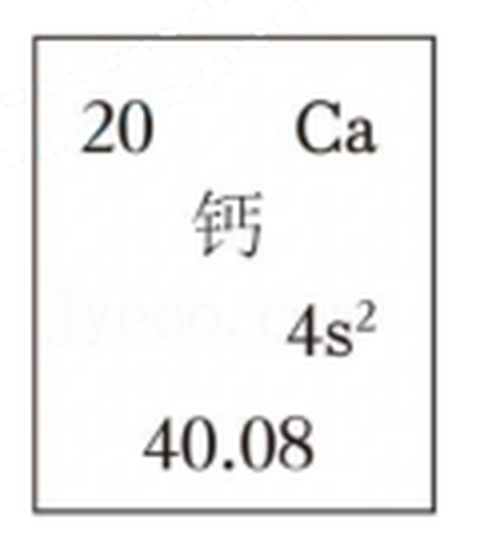
\includegraphics[width=1.7cm]{figures/ca_element_box.png}
\end{center}

\choicepairs
  {如图中 40.08 指钙元素的相对原子质量}
  {${}^{41}\mathrm{Ca}$ 的半衰期长，说明 ${}^{41}\mathrm{Ca}$ 难以失去电子}
  {${}^{41}\mathrm{Ca}$ 的衰变速度小于 ${}^{14}\mathrm{C}$ 的衰变速度}
  {从 Ca 原子束流中直接俘获 ${}^{41}\mathrm{Ca}$ 原子的过程属于化学变化}
\end{enumerate}

%==========================================================
\bigsection{二、胶体化学（本题共 16 分）}

\noindent\textbf{2.（16 分）}胶体在生命科学、材料科学及环境科学中具有广泛应用。近年来，各向异性胶体组装、生物大分子稳定性等研究为胶体化学开辟了新方向。

\begin{enumerate}[label=（\arabic*）]
\item 下列有关胶体的叙述中，正确的是\blank[3em]。
\choicelines
  {胶体区别于溶液的本质特征是胶体能够产生丁达尔现象}
  {将饱和 \ch{FeCl3} 溶液直接加热煮沸可制得 \ch{Fe(OH)3} 胶体}
  {不断搅拌后，\ch{Fe(OH)3} 胶体仍然能够稳定存在}
  {明矾[$\mathrm{KAl(SO_4)_2\cdot 12H_2O}$]可用于净水是利用了胶体粒子具有较好的吸附性}

\item 复核实验小组设计不同的实验对其制得的 \ch{Fe(OH)3} 胶体进行性质探究。写出制备 \ch{Fe(OH)3} 胶体的化学方程式：\blank[9em]。

\item 提纯制得的 \ch{Fe(OH)3} 胶体的装置是如图中的\blank[2.6em]。

\begin{center}
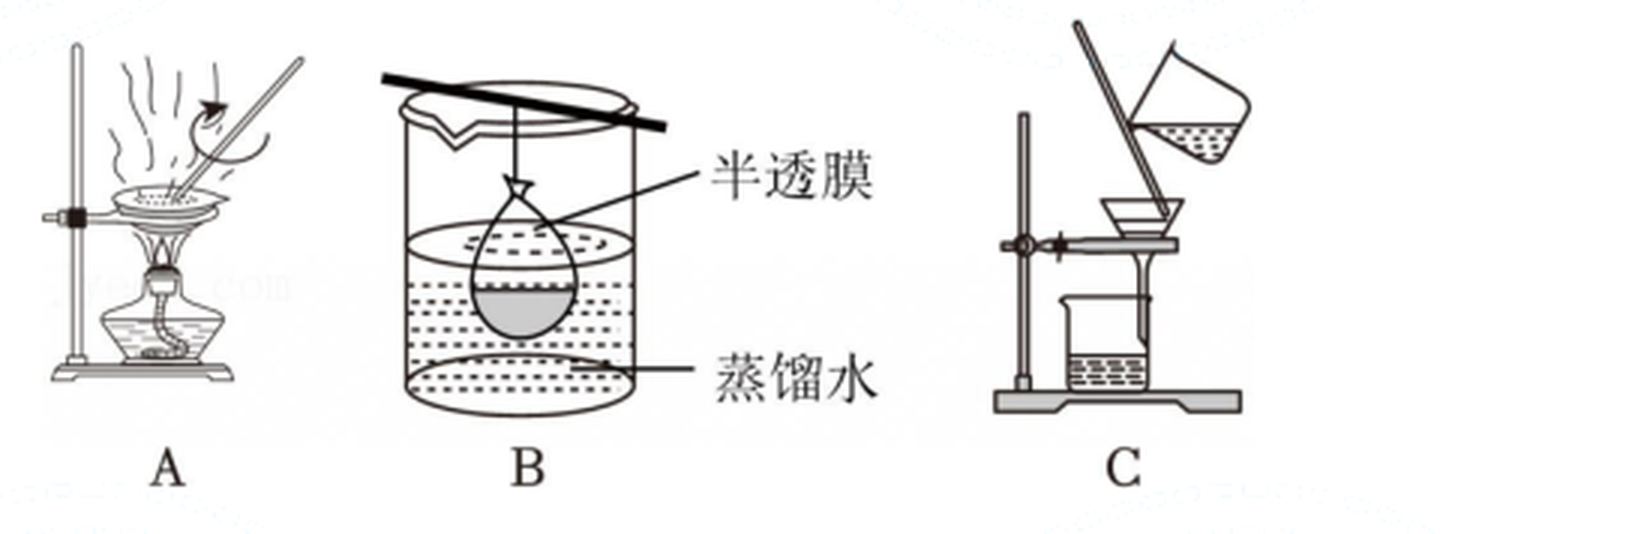
\includegraphics[width=0.80\textwidth]{figures/feoh3_purify.png}
\end{center}

\item 将提纯后的 \ch{Fe(OH)3} 胶体置于 U 形管中，通直流电一段时间后，观察到\blank[2.8em]（填“阳极”或“阴极”）附近红褐色加深，该现象称为\blank[3.4em]。

研究表明，\ch{Fe(OH)3} 胶体可净化水中低浓度的砷酸（\ch{H3AsO4}）。如图所示是不同 pH 时 \ch{Fe(OH)3} 胶体对低浓度砷酸的吸附效率曲线。

\begin{center}
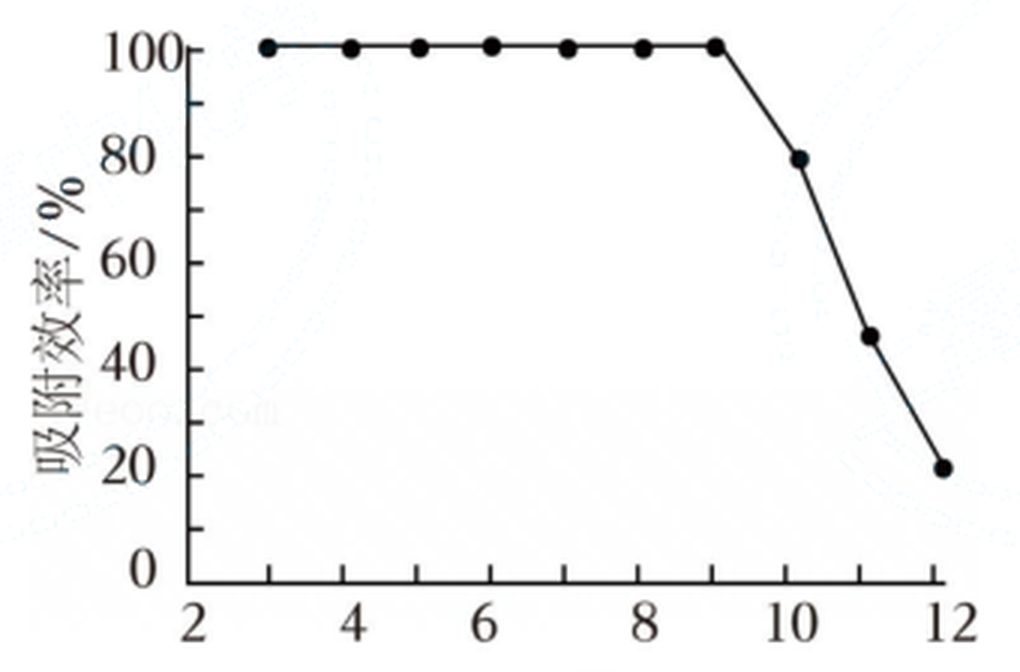
\includegraphics[width=0.42\textwidth]{figures/as_adsorption_ph.png}
\end{center}

已知：pH 反映溶液的酸碱性，pH 越高，溶液的碱性越强。pH 为 $3\sim 9$ 时，溶液中的含砷微粒主要是 $\mathrm{H_2AsO_4^-}$、$\mathrm{HAsO_4^{2-}}$。

\item pH 为 $3\sim 9$ 时，\ch{Fe(OH)3} 胶体对砷酸的吸附效率较高，其可能的原因是\blank[8em]。

\item 当水中砷酸浓度较高时，\ch{Fe(OH)3} 胶体将直接与砷酸发生化学反应生成砷酸铁（\ch{FeAsO4}）沉淀，其中砷元素是\blank[2.6em]价。$\mathrm{AsO_4^{3-}}$ 是酸根离子，则 \ch{FeAsO4} 属于\blank[3em]（填“酸”“碱”“盐”或“氧化物”）。

\item 2025 年《Nature》刊载了南方科技大学罗智团队关于氨基酸稳定胶体机制的研究。该研究发现，氨基酸（如脯氨酸、甘氨酸等）可作为稳定剂，通过吸引屏蔽机制，可逆地吸附在蛋白质、DNA 或纳米颗粒等胶体粒子的特定表面位点，削弱胶体粒子间的吸引力，从而显著提升胶体分散系的稳定性。这与电解质（如 \ch{NaCl}、\ch{Na2SO4} 等）促使胶体聚沉的作用机制相反。电解质（如 \ch{NaCl}、\ch{Na2SO4} 等）促使胶体聚沉的作用机制是\blank[8em]。

\item 蛋白药物制剂属于胶体分散系，其常常因蛋白质的相互聚集而失去药效。为了延长药物的有效期，免疫球蛋白制剂（如 Cuvitru\textsuperscript{\textregistered}）中常添加脯氨酸和甘氨酸。根据上述研究，阐述其延长有效期的主要原理是\blank[8em]。
\end{enumerate}

%==========================================================
\bigsection{三、海洋资源（本题共 25 分）}

\noindent\textbf{3.（25 分）}海洋是一座资源的宝库，化学工业中的许多基础原料都来自海洋。

\begin{enumerate}[label=（\arabic*）]
\item 海水淡化可缓解淡水资源匮乏问题。如图为太阳能海水淡化装置，该装置利用的原理是\blank[3.8em]（填分离操作名称）。

\begin{center}
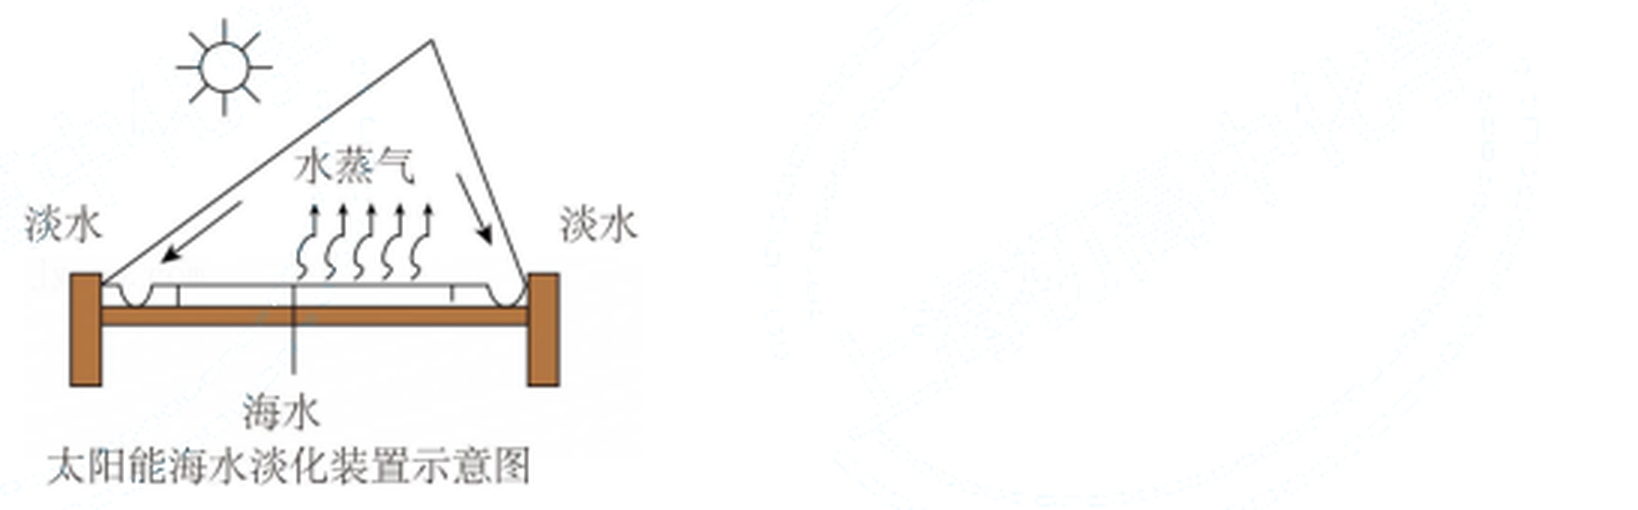
\includegraphics[width=0.52\textwidth]{figures/solar_desalination.png}
\end{center}

\item 利用海洋资源海带可以提取碘。实验室采用“萃取分液”的方法分离碘单质与有机溶剂。以下相关操作错误的是\blank[2.6em]。
% 注：该四联图中的第四个标签原卷即误印为「B.分液」（应为 D.分液），此处照原卷保留，未作改动。

\begin{center}
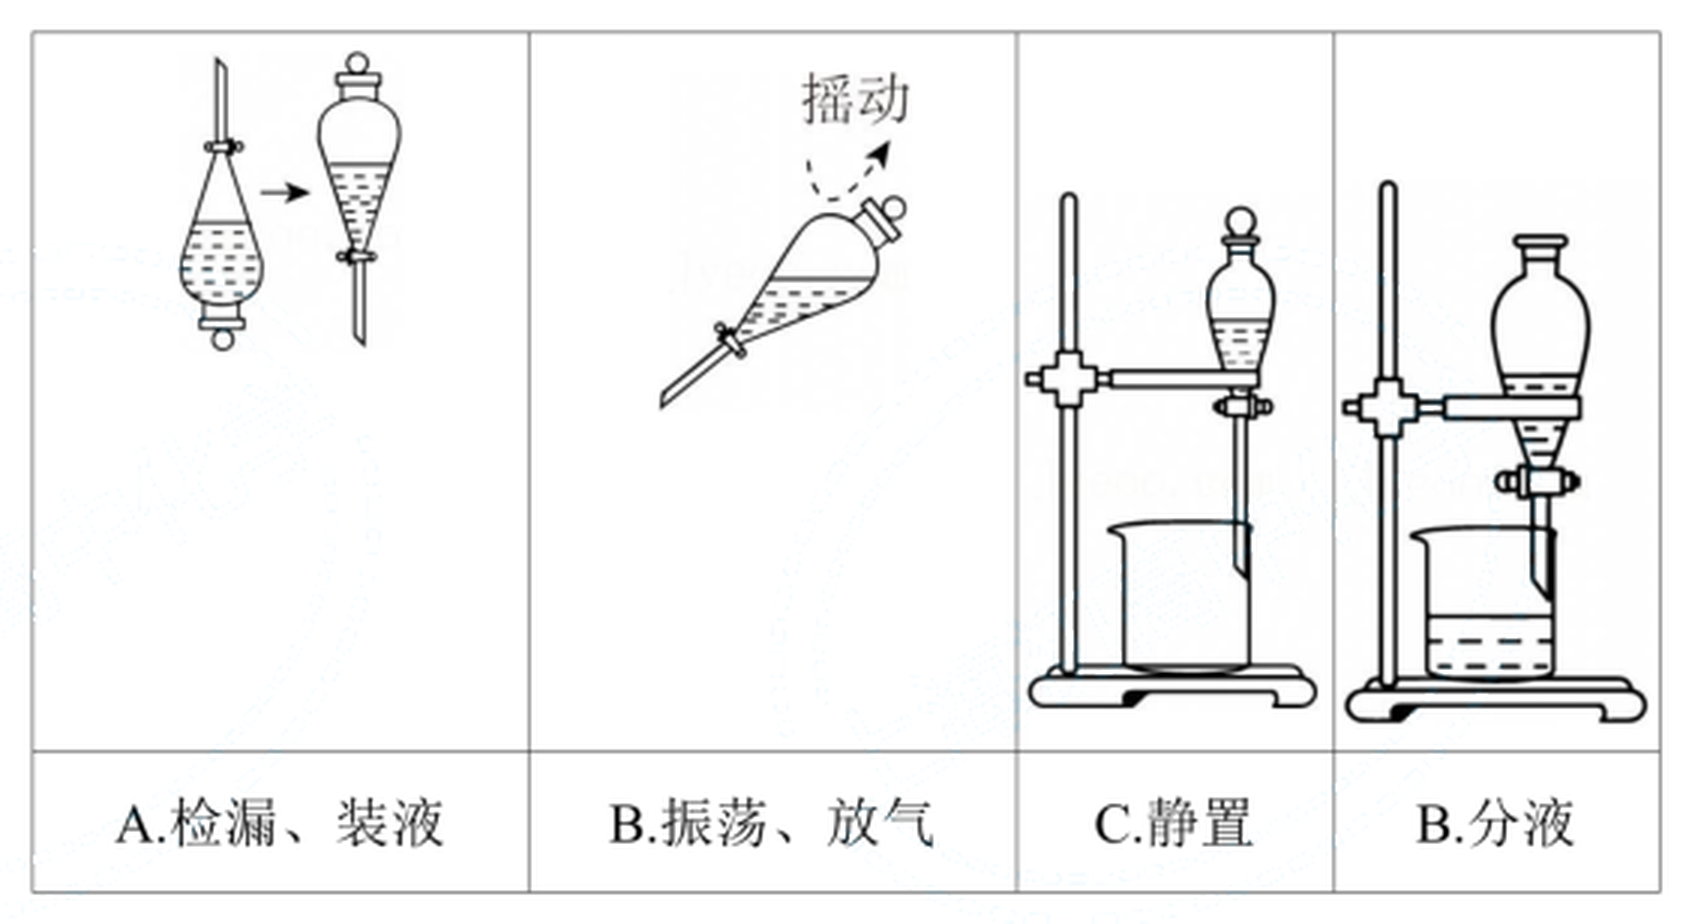
\includegraphics[width=0.68\textwidth]{figures/iodine_extraction.png}
\end{center}

\item 萃取碘水中的碘单质，可以选择的萃取剂种类很多，但不包括\blank[3em]（不定项）。
\choice{酒精}{四氯化碳}{苯}{\ch{NaCl} 溶液}

$\mathrm{SO_4^{2-}}$ 是海洋中硫元素的主要存在形式之一，其存在会干扰海水中 $\mathrm{Cl^-}$ 的检验。

\item 检验海水中 $\mathrm{Cl^-}$ 的方法是\blank[10em]。

\item 某 \ch{Na2SO4} 溶液中含有少量 \ch{Na2CO3}，已知 \ch{Na2SO4} 和 \ch{Na2CO3} 的溶解度曲线如图所示，则从该溶液中获得 $\mathrm{Na_2SO_4\cdot 10H_2O}$ 的操作是加入\blank[5em]后，\blank[4em]、\blank[4em]、过滤、洗涤、干燥。

\begin{center}
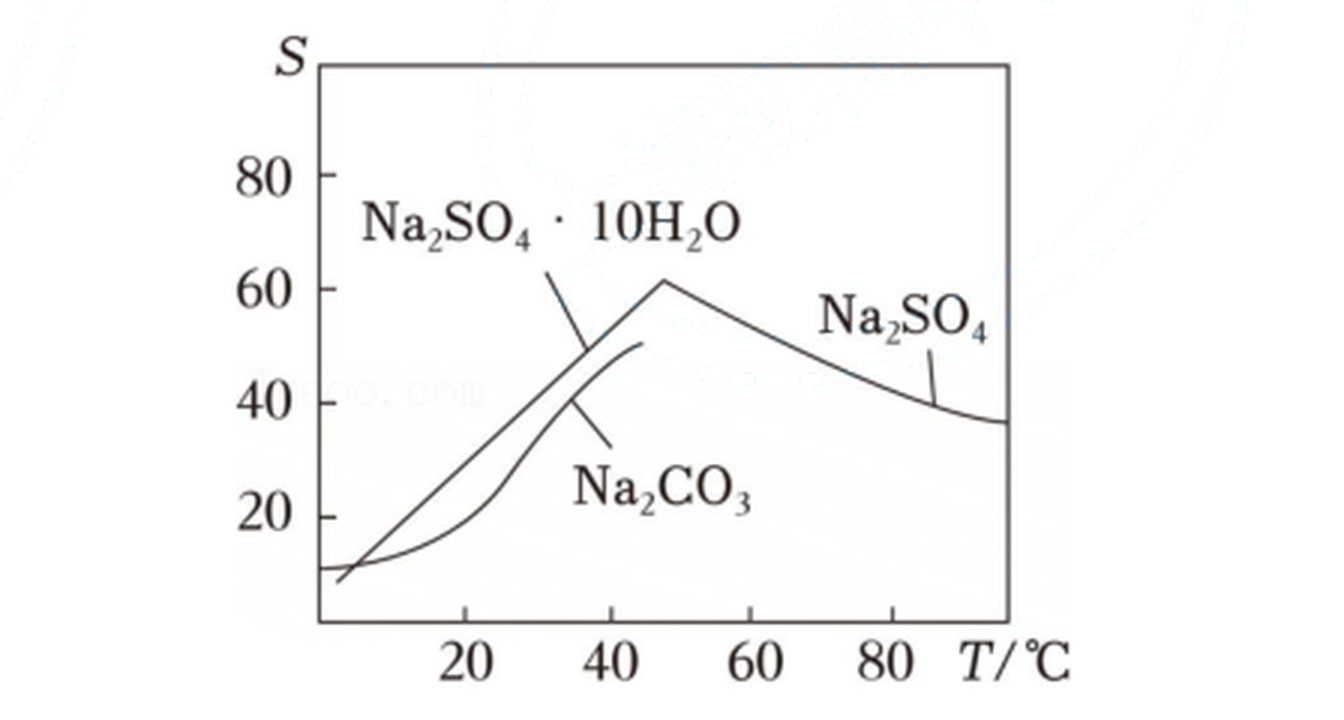
\includegraphics[width=0.48\textwidth]{figures/solubility_na2so4.png}
\end{center}

\item 以海水为原料可制取“84”消毒液。如图所示为某市售“84”消毒液标签上的部分数据，请回答下列问题。

\begin{center}
\begin{tabular}{|l|}
\hline
\rule{0pt}{1.3em}【有效成分】\ch{NaClO} \\
\hline
\rule{0pt}{1.3em}【质量分数】24\% \\
\hline
\rule{0pt}{1.3em}【溶液密度】1.18 g/cm\textsuperscript{3} \\
\hline
\rule{0pt}{1.3em}【净含量】1000 mL \\
\hline
\end{tabular}
\end{center}

该“84”消毒液的物质的量浓度约为\blank[3.4em] mol$\cdot$L\textsuperscript{$-$1}（结果保留 1 位小数）。

\item \textcircled{1} 欲配制 80 mL 2.000 mol$\cdot$L\textsuperscript{$-$1} \ch{NaClO} 溶液，需准确称量 \ch{NaClO} 固体\blank[3.4em] g。

\textcircled{2} 配制该溶液过程中所用玻璃仪器有烧杯、玻璃棒、\blank[6em]（填仪器名称）。

\item 如图是配制溶液的几个关键实验步骤和操作。

\begin{center}
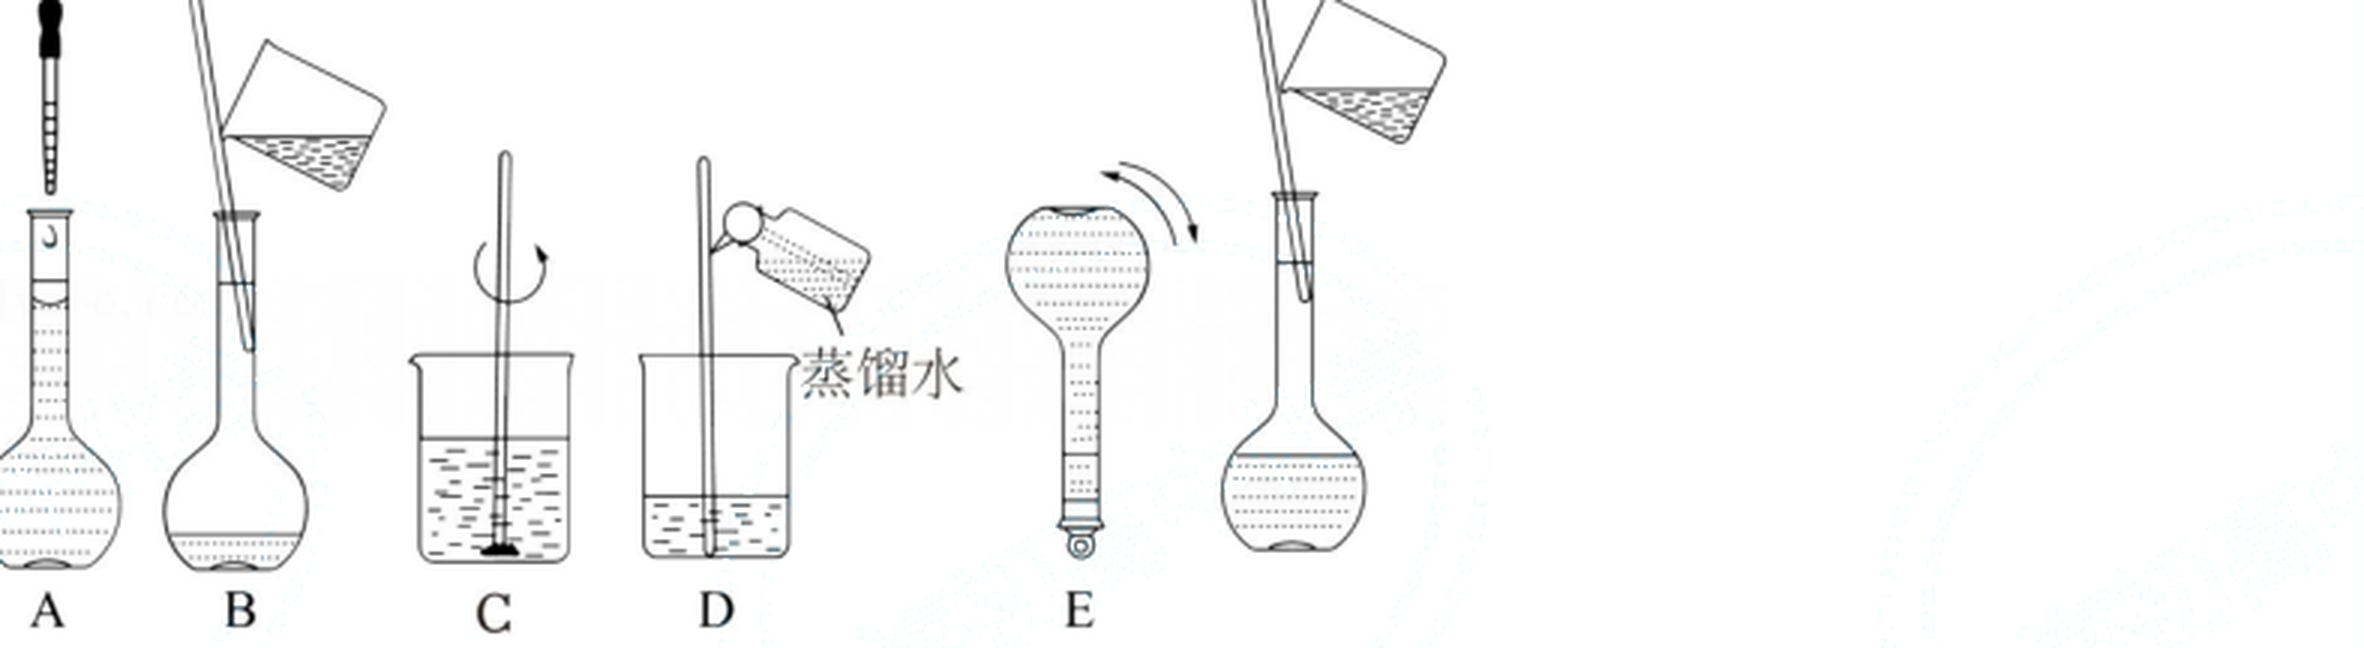
\includegraphics[width=0.88\textwidth]{figures/dilution_steps.png}
\end{center}

将上述实验步骤 A$\sim$E 按实验过程先后次序排列\blank[6em]。

\item 若所配制的次氯酸钠溶液浓度偏低，原因可能是\blank[3em]（不定项）。
\choicelines
  {配制前，容量瓶中有少量蒸馏水}
  {洗涤液未转移到容量瓶中}
  {定容时，仰视刻度线}
  {定容摇匀后，有少量溶液外流}

\item “84”消毒液与稀硫酸混合使用可增强消毒能力，某消毒小组人员用 98\%（密度为 1.84 g$\cdot$cm\textsuperscript{$-$3}）的浓硫酸配制 250 mL 2.3 mol$\cdot$L\textsuperscript{$-$1} 的稀硫酸用于增强“84”消毒液的消毒能力。需要浓硫酸的体积为\blank[3.4em] mL（保留 1 位小数）。

\item 若在用浓硫酸配制稀硫酸时，将量筒、烧杯、玻璃棒均洗涤 $2\sim 3$ 次，并将洗涤液转入容量瓶，会造成所配制的稀硫酸的浓度\blank[2.6em]。
\choicethree{偏高}{偏低}{无影响}
\end{enumerate}

%==========================================================
\bigsection{四、\ch{CuSO4} 溶液（本题共 19 分）}

\noindent\textbf{4.（19 分）}旦旦实验小组为测定 \ch{CuSO4} 溶液的浓度，设计了两个方案。

\noindentⅠ. 甲方案：取 25 mL \ch{CuSO4} 溶液，加入足量 \ch{BaCl2} 溶液，待沉淀完全后，经过滤、洗涤、干燥，得到干燥纯净的 \ch{BaSO4}，称量。

\begin{enumerate}[label=（\arabic*）]
\item 若固体质量为 $w$ g，则 $c(\mathrm{CuSO_4})=$\blank[7em] mol$\cdot$L\textsuperscript{$-$1}（不用化简）。

\item[] \noindentⅡ. 乙方案。实验步骤：

\begin{center}
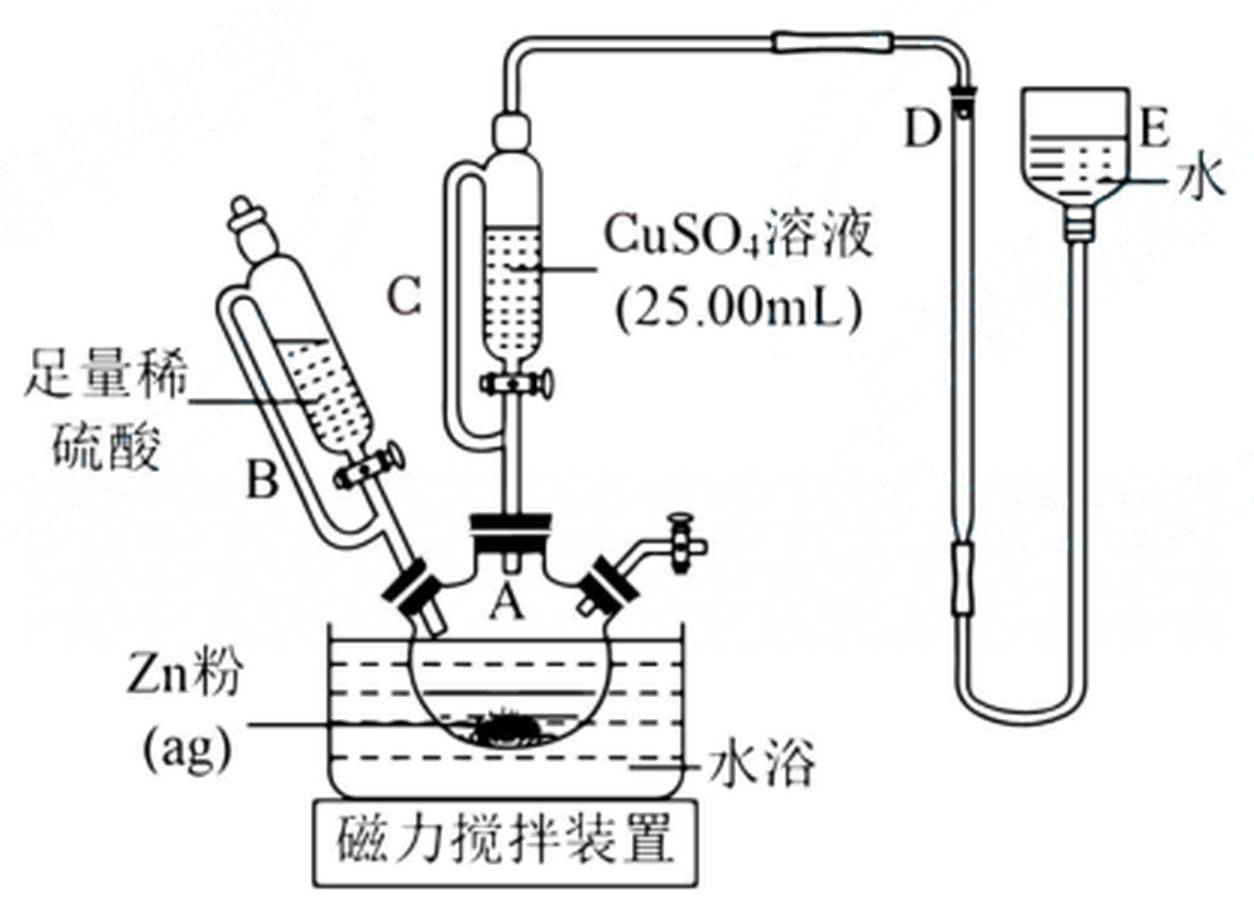
\includegraphics[width=0.46\textwidth]{figures/h2_volume_apparatus.png}
\end{center}

\begin{enumerate}[label=\textcircled{\arabic*},leftmargin=2.6em,itemsep=0.2em,topsep=0.2em]
\item 按如图安装装置（加持仪器略去）
\item ……
\item 在仪器 A、B、C、D、E 中加入如图所示的试剂
\item 调整 D、E 中两液面相平，使 D 中液面保持在 0 或略低于 0 的刻度位置，读数并记录
\item 将 \ch{CuSO4} 溶液滴入 A 中并搅拌，反应完成后，再滴加稀硫酸至体系中不再有气体产生
\item 待体系恢复到室温，移动 E 管，保持 D、E 中两液面相平，读数并记录
\item 处理数据
\end{enumerate}

\item 步骤\textcircled{2} 为\blank[8em]。

\item Zn 粉质量为 $a=0.195$ g，若测得 \ch{H2} 体积为 22.40 mL（已折算为标准状况下的体积），则\blank[8em]（写出必要的计算步骤）
\workspace[5]

\item 若步骤\textcircled{6} E 管液面高于 D 管，未调节液面即读数，则测得 $c(\mathrm{CuSO_4})=$\blank[3em]。
\choice{偏大}{偏小}{无影响}{无法判断}

\item 是否能用同样的装置和方法测定 \ch{MgSO4} 的浓度：\blank[2.6em]（填“是”或“否”）原因是\blank[6em]。

\item 如果 \ch{CuSO4} 浓度的参考值为 0.100 mol/L，而测定结果是 0.096 mol/L，则测定的相对偏差为\blank[3em]。

\item \ch{CuSO4} 溶液经过一系列操作，可以获得 $\mathrm{CuSO_4\cdot 5H_2O}$。取 2.50 g $\mathrm{CuSO_4\cdot 5H_2O}$ 受热脱水过程的热重曲线（样品质量随温度变化的曲线）如图所示。

\begin{center}
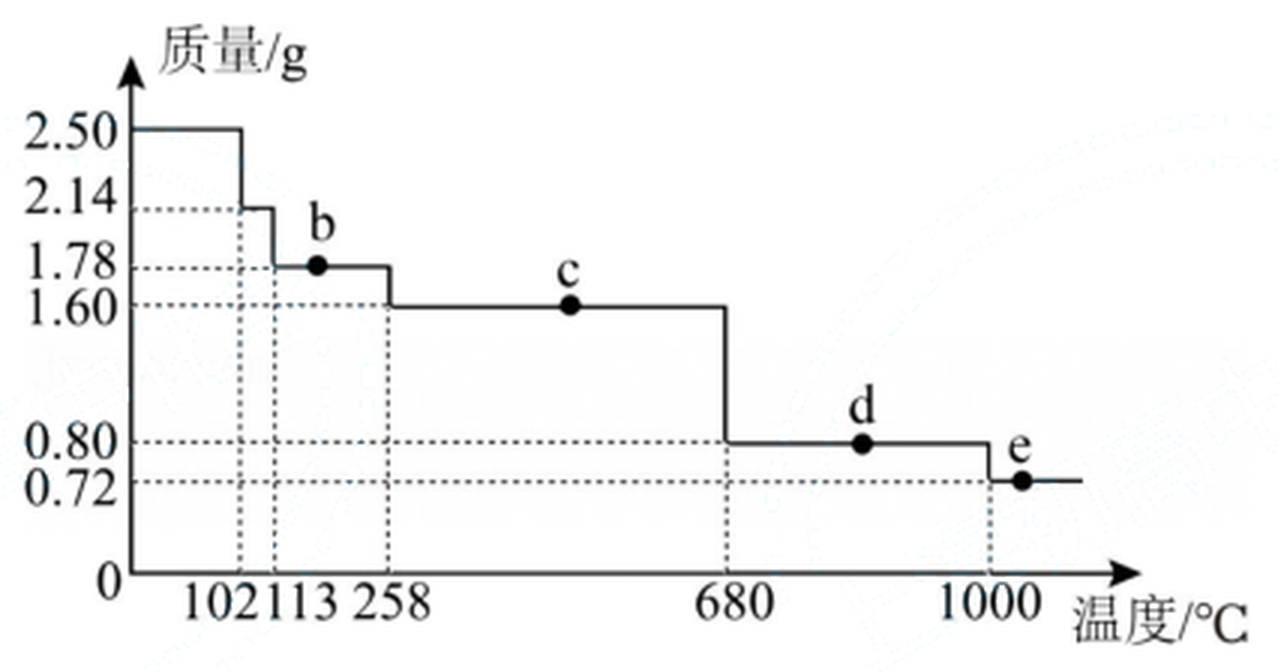
\includegraphics[width=0.48\textwidth]{figures/tga_cuso4.png}
\end{center}

请回答下列问题：b 点时固体物质的化学式\blank[5em]。

\item 取 270 ℃ 所得样品，于 770 ℃ 灼烧得到的主要产物是黑色粉末和 \ch{SO3}，该反应的化学方程式为\blank[9em]。

\item 1000 ℃ 发生反应的化学方程式为\blank[9em]。
\end{enumerate}

%==========================================================
\bigsection{五、物质的量（本题共 16 分）}

\noindent\textbf{5.（16 分）}物质的量是将微观粒子数与宏观可称量物理量联系起来的桥梁，极大地促进了化学学科的发展。

\begin{enumerate}[label=（\arabic*）]
\item 某次高空探测，收集到含 \ch{O3}、\ch{O2}、\ch{N2}（其他气体忽略不计）的大气样本，在实验室中微热一段时间后，\ch{O3} 全部转化为 \ch{O2}（$2\mathrm{O_3}=3\mathrm{O_2}$）。若气体总体积增加了 0.36\%，则大气样本中 \ch{O3} 的体积分数为\blank[3.4em]（反应前后温度和压强均保持不变）。

\item 物质 R 吸收氢气后成为 $\mathrm{RH_6}$，$\mathrm{RH_6}$ 晶体中的氢密度可达到 $1.1\times 10^{3}$ g$\cdot$m\textsuperscript{$-$3}（氢密度是指单位体积晶体中氢元素的质量），则此时 1 m\textsuperscript{3} 晶体中所储的氢相当于标准状况下\blank[5em] L 氢气。

\item 如图所示，一密闭容器被无摩擦、可自由滑动的两隔板 a、b 分成甲、乙两室；标准状况下，在乙室中充入 \ch{NH3} 0.4 mol，甲室中充入 \ch{HCl}、\ch{N2} 的混合气体，静止时隔板位置如图所示。已知甲、乙两室中气体的质量差为 17.3 g。

\begin{center}
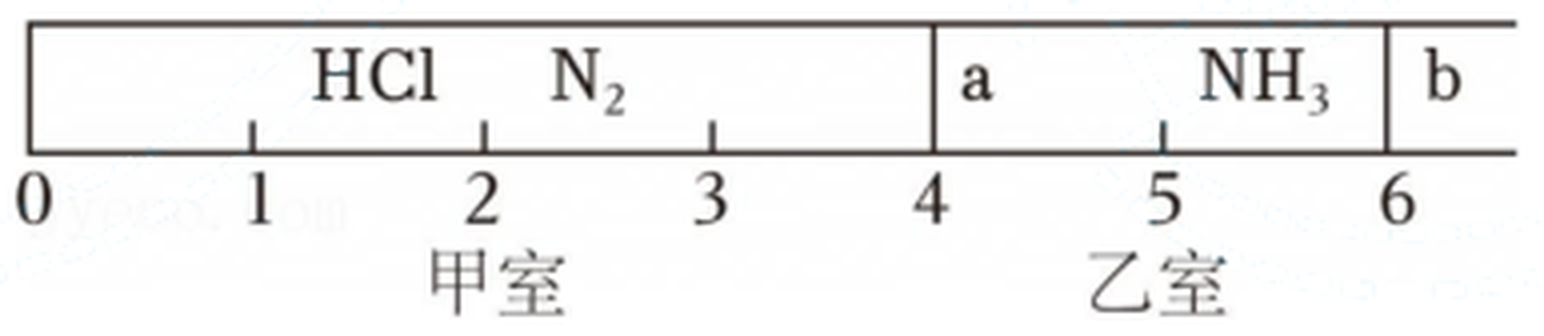
\includegraphics[width=0.62\textwidth]{figures/two_chamber_tube.png}
\end{center}

\textcircled{1} 甲室中气体总质量为\blank[3.4em] g。

\textcircled{2} 甲室中 \ch{HCl}、\ch{N2} 的物质的量之比为\blank[3em]。

\textcircled{3} 将隔板 a 去掉，当 \ch{HCl} 与 \ch{NH3} 充分反应生成 \ch{NH4Cl} 固体后（仅发生此反应），隔板 b 将位于刻度“\blank[3em]”处（填数字，不考虑固体物质产生的体积），此时体系的平均相对分子质量为\blank[3.4em]。

\item 火箭发射后，发射场附近废水中偏二甲肼（\ch{C2H8N2}）浓度变高，可用 \ch{H2O2} 对废水处理。处理 100 L 的 2000 mg/L 偏二甲肼废水，使用密度为 1.11 g/mL 30\% 的 \ch{H2O2} 溶液，则 \ch{H2O2} 溶液的理论投加量为\blank[3.4em] L（保留两位小数）。

已知：$\mathrm{C_2H_8N_2(l)+8H_2O_2(l)=N_2(g)+2CO_2(g)+12H_2O(l)}$

\item 焦亚硫酸钠（\ch{Na2S2O5}）易溶于水，与强酸反应放出较多 \ch{SO2}。\ch{Na2S2O5} 作为食品添加剂，在葡萄酒中残留量一般不得超过 0.25 g$\cdot$L\textsuperscript{$-$1}（以 \ch{SO2} 计）。小复同学检测葡萄酒样品中 \ch{Na2S2O5} 残留量，实验如下：取 150 mL 葡萄酒样品，加稀硫酸酸化后加热，将产生气体通入足量双氧水中充分吸收，再除去过量的 \ch{H2O2}，冷却后，用 0.100 mol$\cdot$L\textsuperscript{$-$1} \ch{NaOH} 溶液与上述吸收液反应，恰好反应时消耗 \ch{NaOH} 溶液 15.00 mL，则该样品中 \ch{Na2S2O5} 的残留量为\blank[4em] g$\cdot$L\textsuperscript{$-$1}（残留量以 \ch{SO2} 计）。

已知：$\mathrm{SO_2+H_2O_2=H_2SO_4}$
\workspace[6]
\end{enumerate}

%==========================================================
% 以下「参考答案」整节仅在答案版输出（试卷版由 \ifanswer 整段吞掉）
\ifanswer
\newpage
\bigsection{参考答案}

\begin{enumerate}[label=\textbf{\arabic*.},leftmargin=2.5em]
\item
\begin{enumerate}[label=（\arabic*）]
\item D；
\item $A-x+n+24$；
\item B；
\item C；
\item AD（不定项）；
\item 氚。A 为氢元素，其核素中质子数（1）为中子数（2）的一半，即 ${}_{1}^{3}\mathrm{H}$；
\item $\left[\mathrm{H}:\right]^-$（$\mathrm{H^-}$ 的电子式）；$\mathrm{Mg^{2+}}$ 的结构示意图为
\begin{center}
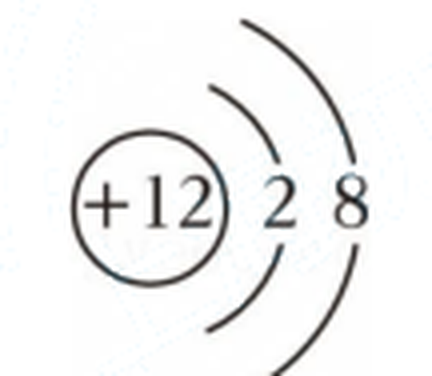
\includegraphics[width=1.1cm]{figures/mg2_plus_shell.png}
\end{center}
\item $\mathrm{SO_2+2NaOH=Na_2SO_3+H_2O}$（$EB_2$ 为 \ch{SO2}，$CBA$ 为 \ch{NaOH}）；
\item $a=7.58$，$b=49.82$；
\item AC（不定项）。
\end{enumerate}

\item
\begin{enumerate}[label=（\arabic*）]
\item D；
\item $\mathrm{FeCl_3+3H_2O}\xrightarrow{\Delta}\mathrm{Fe(OH)_3(\text{胶体})+3HCl}$；% \Delta 不可写在 \mathrm{} 内，否则映射到 Times New Roman 缺字形
\item B；
\item 阴极；电泳；
\item pH 为 $3\sim 9$ 时，溶液中的含砷微粒主要是 $\mathrm{H_2AsO_4^-}$、$\mathrm{HAsO_4^{2-}}$，\ch{Fe(OH)3} 胶体粒子带正电荷，能吸附带负电荷的 $\mathrm{H_2AsO_4^-}$、$\mathrm{HAsO_4^{2-}}$；
\item $+5$ 价；盐；
\item 向胶体中加入盐时，其中的阳离子或阴离子能中和分散质微粒所带的电荷，从而使分散质聚集成较大的微粒，在重力作用下形成沉淀析出；
\item 氨基酸通过阻碍颗粒间直接接触，增强胶体颗粒间的排斥作用来抑制胶体聚集。
\end{enumerate}

\item
\begin{enumerate}[label=（\arabic*）]
\item 蒸馏（填分离操作名称）；
\item B；
\item AD（不定项）；
\item 取少量海水于试管中，向其中加入 \ch{Ba(NO3)2} 溶液，静置，向上层清液中（或取上层清液）加入 \ch{HNO3} 酸化的 \ch{AgNO3} 溶液，若有白色沉淀生成，说明海水中有 $\mathrm{Cl^-}$；
\item 硫酸至不再产生气泡；蒸发浓缩、冷却结晶；
\item 3.8 mol$\cdot$L\textsuperscript{$-$1}（结果保留 1 位小数）；
\item \textcircled{1} 14.9 g；\textcircled{2} 胶头滴管、100 mL 容量瓶（填仪器名称）；
\item CBDBAE；
\item BC（不定项）；
\item 31.3 mL（保留 1 位小数）；
\item A。
\end{enumerate}

\item
\begin{enumerate}[label=（\arabic*）]
\item $\dfrac{40w}{233}$ mol$\cdot$L\textsuperscript{$-$1}（不用化简）；
\item 检查装置的气密性；
\item $0.08$ mol/L（写出必要的计算步骤）；
\item A；
\item 否（填“是”或“否”）；原因是 Mg 比 Zn 活泼，Zn 与 \ch{MgSO4} 不反应；
\item 4\%；
\item $\mathrm{CuSO_4\cdot H_2O}$；
\item $\mathrm{CuSO_4\xrightarrow{770\,^{\circ}\mathrm{C}}CuO+SO_3\uparrow}$；
\item $\mathrm{4CuO\xrightarrow{1000\,^{\circ}\mathrm{C}}2Cu_2O+O_2\uparrow}$。
\end{enumerate}

\item
\begin{enumerate}[label=（\arabic*）]
\item 0.72\%（反应前后温度和压强均保持不变）；
\item $1.232\times 10^{6}$ L 氢气；
\item \textcircled{1} 24.1 g；\textcircled{2} $1:3$；\textcircled{3} 4；25.25；
\item 2.72 L（保留两位小数）；
\item 0.320 g$\cdot$L\textsuperscript{$-$1}（残留量以 \ch{SO2} 计）。
\end{enumerate}
\end{enumerate}
\fi

\end{document}
